\documentclass[a4paper,12pt]{report}
%\usepackage{biblatex}
%\usepackage[sectionbib]{chapterbib}%%% REFERENCE PAR CHARPITRE %%%
\usepackage[french,english]{babel}
\usepackage[nottoc]{tocbibind} 
\frenchbsetup{StandardLists=true}
\usepackage{enumitem}
\usepackage{tikz}
\usepackage{pgfplots}
%\usepackage[glenn]{fncychap}
% chargement des packages necessaire pour les code/script
\usepackage{tcolorbox}
\usepackage{listings,xcolor}
\usepackage{fancyhdr}
\usepackage{multirow}
\usepackage{booktabs}
% chargement des packages pour les tableaux
\usepackage{verbatim}
\usepackage{multirow} %
\usepackage{colortbl} %
\usepackage{spreadtab}
\usepackage{booktabs}
\usepackage{slashbox}
\usepackage{fancybox,ctable}
\usepackage{xstring}
\usepackage{float} 
\usepackage[T1]{fontenc}
\usepackage[utf8]{inputenc}
\usepackage{lmodern}
\usepackage{microtype}
\usepackage{amsmath}
\usepackage{graphicx}
\usepackage[font={small}]{caption}
%\usepackage[light, largesmallcaps]{kpfonts}%%%% LE FONT DE BASE DU TEXTE %%%%
\usepackage[top=2.5cm, bottom=2cm, left=3cm, right=2.5cm,
			headheight=15pt]{geometry}


\newcommand{\cia}{\begin{figure}[H]
\centering
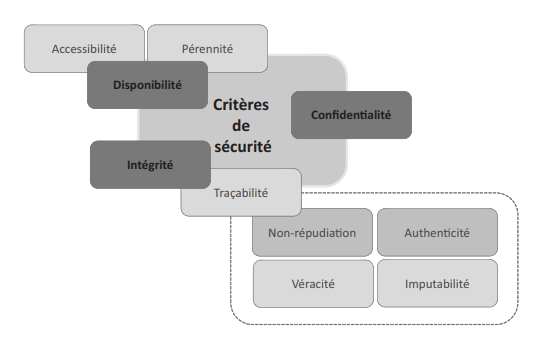
\includegraphics{images/CIA}
\caption{Critères de sécurité informatique \cite{ref4}}
\label{imagecia}
\end{figure}
}

\newcommand{\dl}{\begin{figure}[H]
\centering
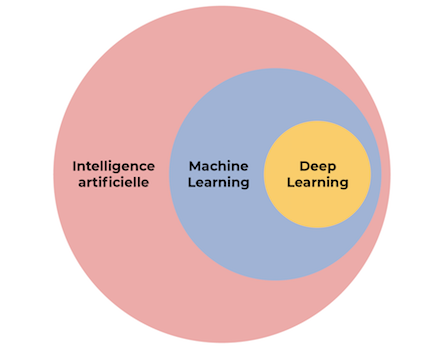
\includegraphics[height=5cm]{images/dl}
\caption{Position du Deep Learning dans l'IA \cite{refclassroom}}
\label{dl}
\end{figure}
}

\newcommand{\nslkdd}{\begin{figure}[H]
\centering
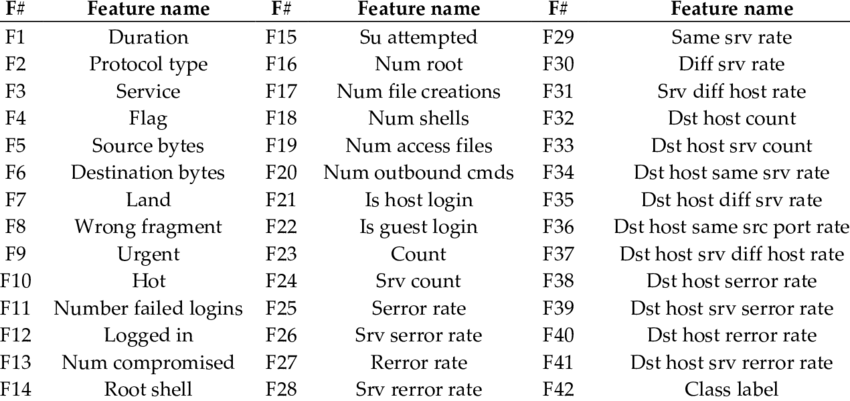
\includegraphics[width=\textwidth]{images/nslkdd}
\caption{Liste des caractéristiques de NSL-KDD. \cite{kdd}}
\label{nslkdd}
\end{figure}
}
\newcommand{\architecture}{\begin{figure}[H]
\centering
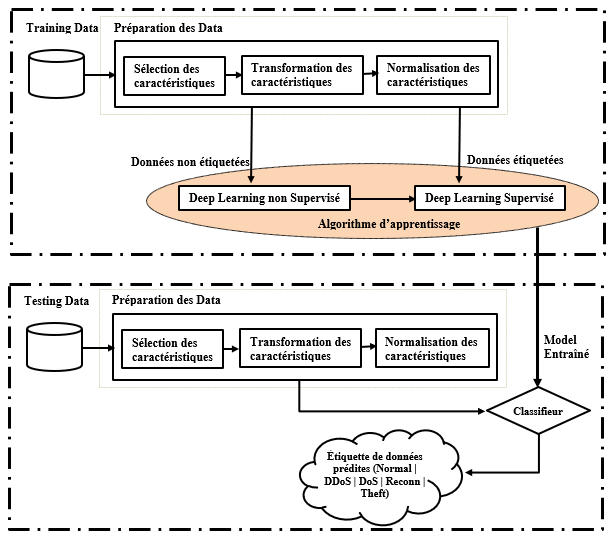
\includegraphics[width=\textwidth]{images/architecture}
\caption{L'architecture de notre approche }
\label{architecture}
\end{figure}
}
\newcommand{\modelAE}{\begin{figure}[H]
\centering
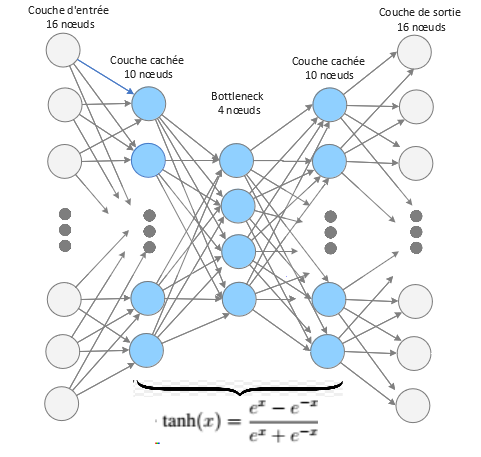
\includegraphics[width=\textwidth]{images/ModelAE}
\caption{Structure de l'AE}
\label{modelAE}
\end{figure}
}
\newcommand{\modelDNN}{\begin{figure}[H]
\centering
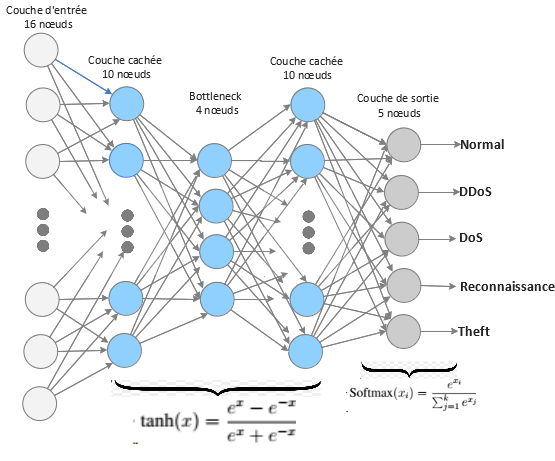
\includegraphics[width=\textwidth]{images/ModelDNN}
\caption{Structure du DNN}
\label{modelDNN}
\end{figure}
}
\newcommand{\iot}{\begin{figure}[H]
\centering
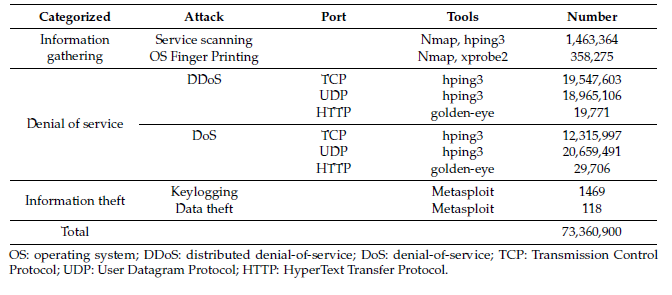
\includegraphics[width=\textwidth]{images/iot}
\caption{Résumé des attaques du Dataset Iot Botnet \cite{kdd}}
\label{nslkdd}
\end{figure}
}
%%%%%%%%%%%%%%%%%%%%%%%%%%%%%%%%%%%

\newcommand{\source}[1]{\caption*{ {#1}} 
}
%\source{\cite{ref4}}

\newcommand{\imageAPS}{\begin{figure}[!h]
\centering
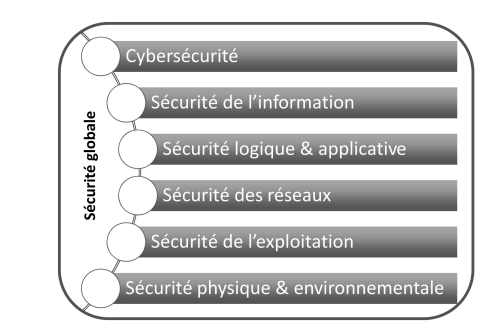
\includegraphics{images/applicationsécurité}
\caption{Application de sécurité informatique \cite{ref4}}
\label{imagecia}
\end{figure}
}

\newcommand{\imgMiM}{\begin{figure}[H]
\centering
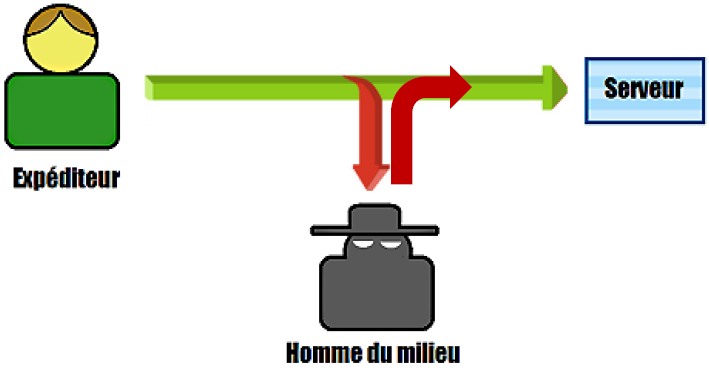
\includegraphics[width=\textwidth]{images/MiM}
\caption{main-in-the-middle}
\label{imagMiM}
\end{figure}
}
\newcommand{\typedl}{\begin{figure}[H]
\centering
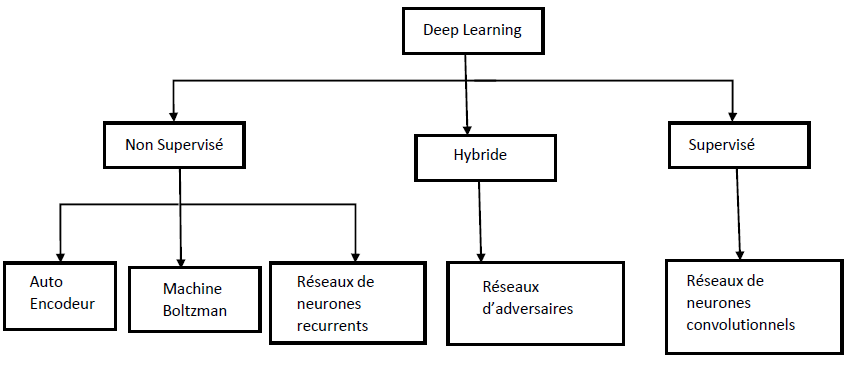
\includegraphics[width=\textwidth]{images/typedl}
\caption{classification des modèles de deep learning}
\label{typedl}
\end{figure}
}

\newcommand{\cnn}{\begin{figure}[H]
\centering
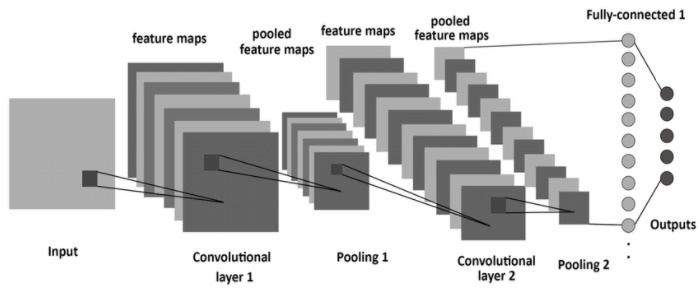
\includegraphics[width=\textwidth]{images/cnn}
\caption{Architecture classique d’un réseau de neurones convolutif \cite{cnn}}
\label{cnn}
\end{figure}
}

\newcommand{\autoencodeur}{\begin{figure}[H]
\centering
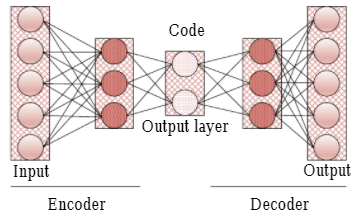
\includegraphics[width=\textwidth]{images/autoencodeur}
\caption{Architecture Auto Encodeur\cite{autoencodeur}}
\label{autoencodeur}
\end{figure}
}

\newcommand{\perceptron}{\begin{figure}[!h]
\centering
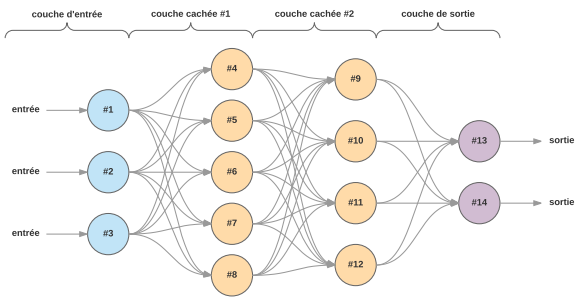
\includegraphics[width=\textwidth]{images/perceptron}
\caption{Réseau de neurone profond (DNN)}
\label{perceptron}
\end{figure}
}

\newcommand{\graphe}{\begin{figure}[H]
\centering
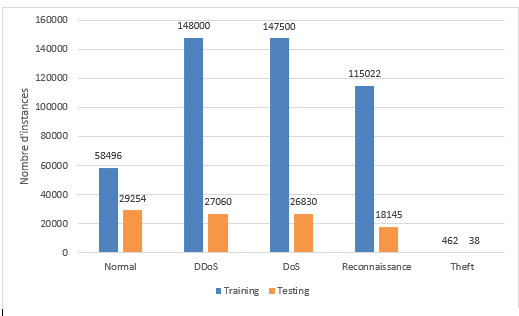
\includegraphics[width=\textwidth]{images/graphe}
\caption{Nombres d'éléments par types de datasets}
\label{graphe}
\end{figure}
}

\newcommand{\neurone}{\begin{figure}[H]
\centering
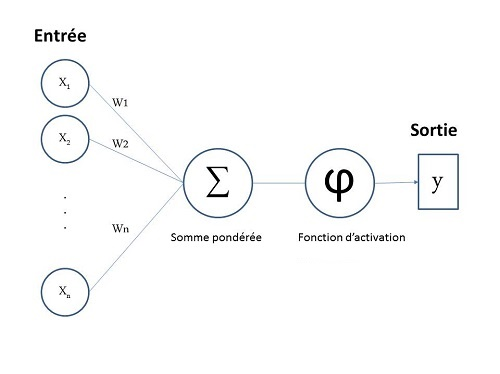
\includegraphics[height=7cm]{images/neuroneF}
\caption{Représentation d'un neurone formel}
\label{atnn}
\end{figure}
}

\newcommand{\cidf}{\begin{figure}[H]
\centering
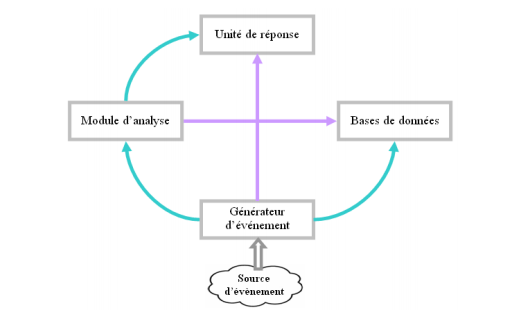
\includegraphics[width=\textwidth]{images/icef}
\caption{l’architecture CIDF \cite{zaidi}}
\label{imagMiM}
\end{figure}
}

\newcommand{\apprentissage}{\begin{figure}[H]
\centering
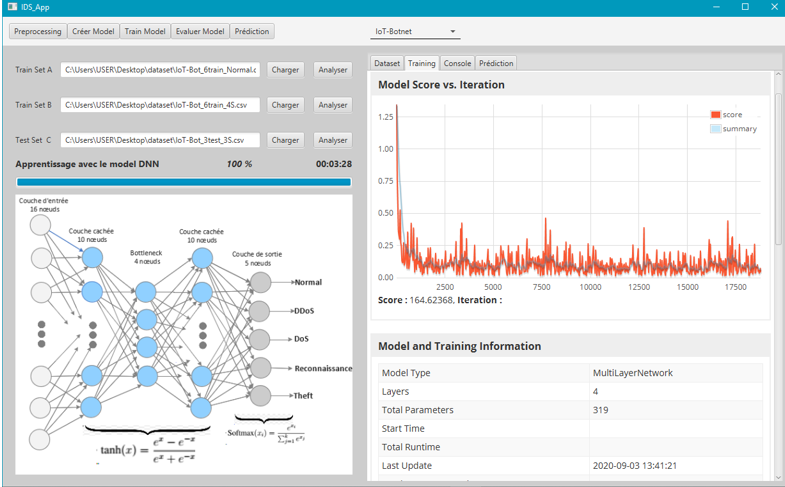
\includegraphics[width=\textwidth]{images/apprentissage}
\caption{Entrainement du modèle DNN}
\label{apprentisage}
\end{figure}
}

\newcommand{\prediction}{\begin{figure}[H]
\centering
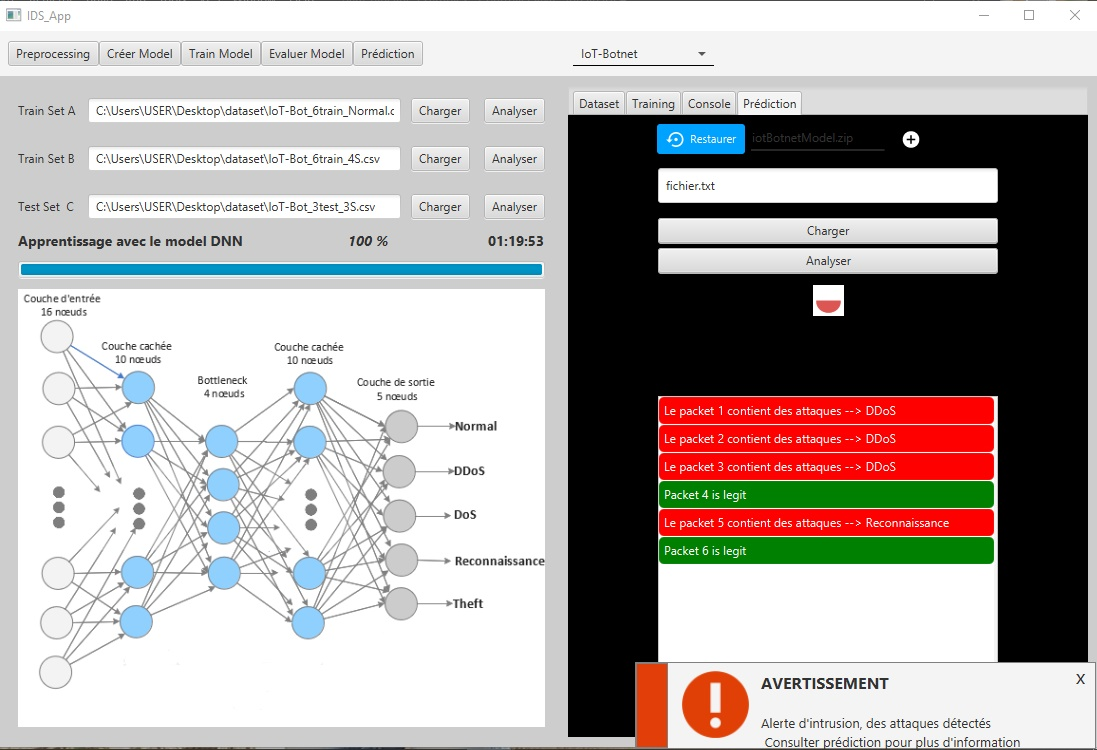
\includegraphics[width=\textwidth]{images/predi}
\caption{prédiction d'attaques}
\label{apprentisage}
\end{figure}
}

\newcommand{\data}{\begin{figure}[H]
\centering
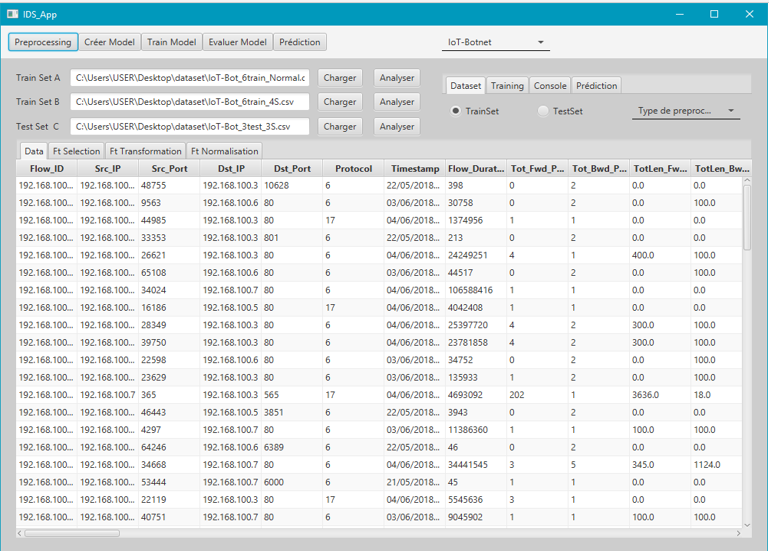
\includegraphics[width=\textwidth]{images/data}
\caption{structure du dataset}
\label{data}
\end{figure}
}

\newcommand{\analyse}{\begin{figure}[H]
\centering
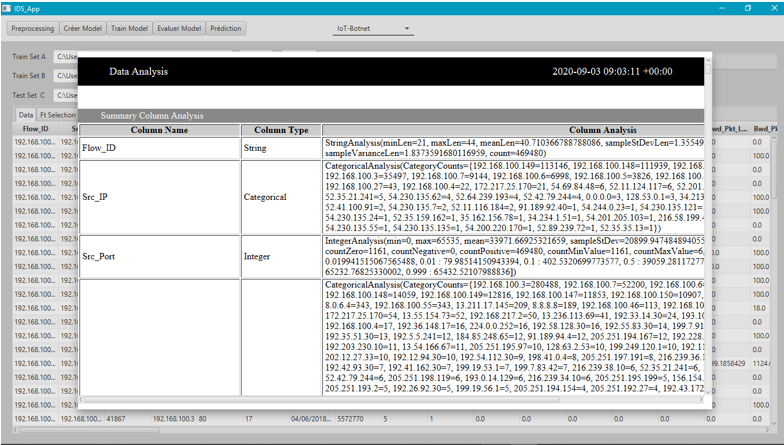
\includegraphics[width=\textwidth]{images/dataanalyse}
\caption{Analyse des données}
\label{data}
\end{figure}
}

\newcommand{\evaluation}{\begin{figure}[H]
\centering
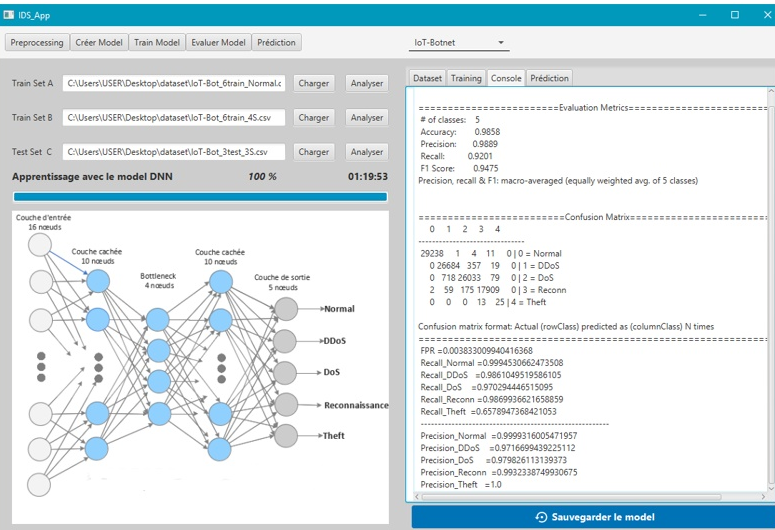
\includegraphics[width=\textwidth]{images/evaluation}
\caption{Evaluation du modèle}
\label{apprentisage}
\end{figure}
}
\newcommand{\idwg}{\begin{figure}[H]
\centering
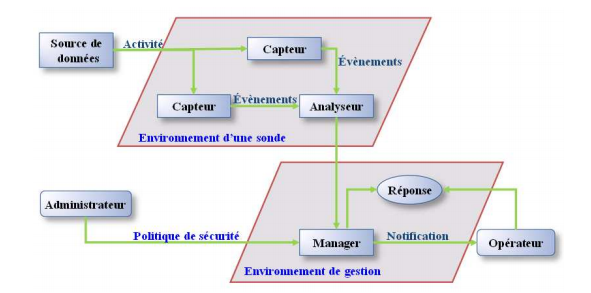
\includegraphics[width=\textwidth]{images/IDWG}
\caption{L’architecture IDWG \cite{zaidi}}
\label{idwg}
\end{figure}
}
\newcommand{\typeids}{\begin{figure}[H]
\centering
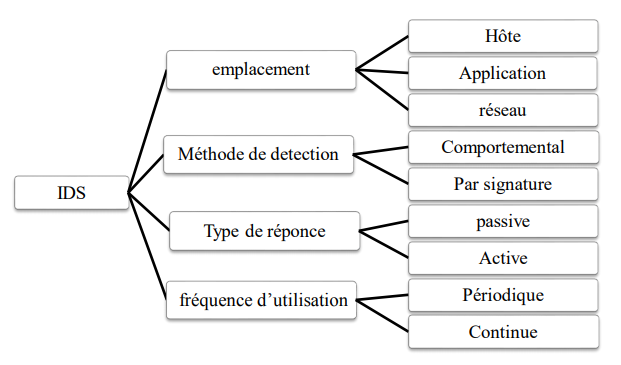
\includegraphics[width=\textwidth]{images/ids}
\caption{Classification des différents types d'IDS  \cite{reftypeids}}
\label{ids}
\end{figure}
}
\newcommand{\hids}{\begin{figure}[H]
\centering
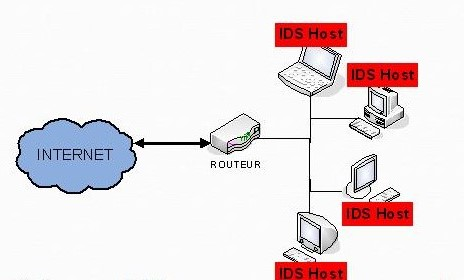
\includegraphics[width=\textwidth,height=10cm]{images/HIDS}
\caption{La détection d'intrusion basée sur l'hôte \cite{refphototypids}}
\label{hids}
\end{figure}
}
\newcommand{\nids}{\begin{figure}[H]
\centering
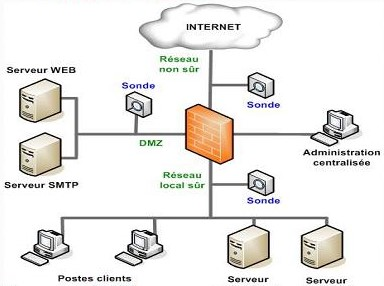
\includegraphics[width=\textwidth,height=10cm]{images/NIDS}
\caption{La Détection d'Intrusion Réseau (NIDS) \cite{refphototypids}}
\label{nids}
\end{figure}
}

\newcommand{\authenti}{\begin{figure}[H]
\centering
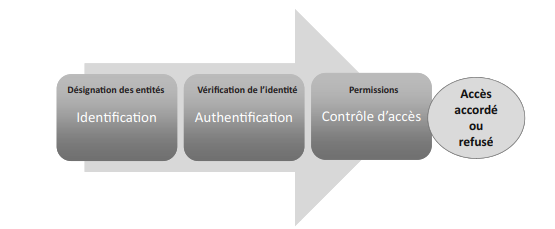
\includegraphics{images/authentification}
\caption{Accès à une ressource \cite{ref4}}
\label{Authentification}
\end{figure}
}

\newcommand{\ransom}{\begin{figure}[H]
\centering

\includegraphics{images/ransomware}
\caption{Ransomware}
\label{ransomware}
\end{figure}
}


\newcommand{\logoucd}{\begin{figure}[!h]
\centering

\includegraphics[width=0.2\linewidth]{Images/uc2}
\label{logo}
\end{figure}
}
\newcommand{\pagedegarde}{
\begin{titlepage}
\newgeometry{top=1.5cm, bottom=1.5cm, left=2cm, right=1cm}
\AddToShipoutPicture*{\EtiquetteThese}
\begin{center}
\begin{minipage}{1\textwidth}
	\begin{center}
		\large\ministere{}
	\end{center}				
\end{minipage}
\vspace{0.9mm}
\logoucd\\
\Huge{\emph{{{\it {Mémoire de fin d'études}}}}}\\
\normalsize
\begin{center}
En vue de l'obtention du Diplôme de\\ 
 \huge{\textbf{MASTER EN INFORMATIQUE}}
\end{center}
\large{\textbf{Option }: Réseaux et Systèmes Distribués}

\vspace{1cm}
\Huge\textbf{Thème }
\noindent\rule{\textwidth}{0.9mm}
%\noindent\color{blueforest}\rule{\textwidth}{0.1mm}
\Large{\textbf{Approche résiliente pour l'identif{\kern0pt}ication et la détection des attaques DDoS dans les réseaux IoT}}
%\noindent\color{blueforest}\rule{\textwidth}{0.1mm}
\noindent\rule{\textwidth}{0.9mm}
\end{center}
\vspace{1.5cm}
\begin{tabular}{l r}
\hspace{1cm}\textbf{Présenté par :}&\hspace{5cm}\textbf{Sous la Direction de :}\\
\hspace{1cm}\textbf{\textcolor{blue}{Japhet DIARRA }}&\textbf{\textcolor{blue}{$M^{r}$ Amir DJENNA}}\\
\hspace{1cm}\textbf{\textcolor{blue}{ Mamadou DIARRA MAKADJI TB}}&\textbf{}
\end{tabular}
\begin{center}
\vspace{1.5cm}
\hspace{0.3cm}\textbf{\large{Devant le jury composé de : }}\\
\vspace{0.5cm}
\begin{tabular}{llll}
%\vspace{0.1cm}
\hspace{0.3cm}\textbf{\textbf{ Président : }} \hspace{0.8cm} $M^{r}$ \textbf{Abdellatif  HABES} \\
\vspace{0.1cm}
\hspace{0.3cm}\textbf{\textbf{Examinatrice : }} \hspace{0.2cm} $M_{me}$ \textbf{Houda  HAFI}
%\hspace{3.1cm} \hspace{0cm} $M^{elle}$ \textsl{XXXX} Xxxx \hspace{2.09cm} \textsl{ \emph{X, Université Constantine 02}}\\
\end{tabular}
\end{center}
\vspace{2cm}
\begin{center}
\textbf{Septembre 2020}
\end{center}
\end{titlepage}
\restoregeometry  
\nopagebreak
}
\newcommand{\firstpart}{\part{\'Etat de l'art}}
\newcommand{\secondpart}{\part{Contributions}}
\newcommand{\ministere}{R\'{e}publique  Alg\'{e}rienne D\'{e}mocratique et Populaire\\Ministère de  l'Enseignement Sup\'{e}rieur et de la Recherche Scientifique\\Université Constantine 2 – Abdelhamid Mehri \\Faculté des Nouvelles Technologies de l'Information et de la Communication (NTIC)\\ Département d’Informatique Fondamentale et ses Applications (IFA)}
\definecolor{blueforest}{RGB}{00,74,09}
\newcommand\EtiquetteThese{%
	\put(-10,10){%
		\parbox[t][\paperheight]{\paperwidth}{%
			\hfill
			\colorbox{blueforest}{		
				\begin{minipage}[b]{3em}
				\vspace{0.1cm}
					\centering\Huge\textcolor{white}{\textbf{M}\\\textbf{A}\\\textbf{S}\\\textbf{T}\\\textbf{E}\\\textbf{ R}}
					\vspace{0.2cm}
				\end{minipage}
			}
		}
	}
}




\usepackage{array}%%%%%%%%%AFFICHAGE DES LETTRES EN VERTICALE
\usepackage{eso-pic}% Nécessaire pour mettre des images en arrière plan
%\usepackage{newtxtext,newtxmath}
%%%%%%%%%%%%%%%%%%%%%%%%%%%%%%%%%%%%%%%%%%%
%           Page de Garde		         %
%%%%%%%%%%%%%%%%%%%%%%%%%%%%%%%%%%%%%%%%%%
\makeatletter 
\def\@specialite{Spécialité}
\newcommand{\specialite}[1]{
  \def\@specialite{#1}
}
\def\@directeur{directeur}
\newcommand{\directeur}[1]{
  \def\@directeur{#1}
}
\def\@encadrant{encadrant}
\newcommand{\encadrant}[1]{
  \def\@encadrant{#1}
}
\def\@jurya{}{}{}
\newcommand{\jurya}[3]{
  \def\@jurya{#1,	& #2	& #3\\}
}
\def\@juryb{}{}{}
\newcommand{\juryb}[3]{
  \def\@juryb{#1,	& #2	& #3\\}
}
\def\@juryc{}{}{}
\newcommand{\juryc}[3]{
  \def\@juryc{#1,	& #2	& #3\\}
}
\def\@juryd{}{}{}
\newcommand{\juryd}[3]{
  \def\@juryd{#1,	& #2	& #3\\}
}
\def\@jurye{}{}{}
\newcommand{\jurye}[3]{
  \def\@jurye{#1,	& #2	& #3\\}
}
\def\@juryf{}{}{}
\newcommand{\juryf}[3]{
  \def\@juryf{#1,	& #2	& #3\\}
}
\def\@juryg{}{}{}
\newcommand{\juryg}[3]{
  \def\@juryg{#1,	& #2	& #3\\}
}
\def\@juryh{}{}{}
\newcommand{\juryh}[3]{
  \def\@juryh{#1,	& #2	& #3\\}
}
\def\@juryi{}{}{}
\newcommand{\juryi}[3]{
  \def\@juryi{#1,	& #2	& #3\\}
}
\makeatother 
\newcommand\EtiquetteThesep{%
	\put(-10,10){%
		\parbox[t][\paperheight]{\paperwidth}{%
			\hfill
			\colorbox{black}{		
				\begin{minipage}[b]{3em}
					\centering\Huge\textcolor{white}{M\\A\\S\\T\\E\\R\\}
					\vspace{0.3cm}
				\end{minipage}
			}
		}
	}
}

\makeatletter
\newcommand{\pagedegardec}{\newgeometry{top=2.5cm, bottom=2cm, left=2cm, right=1cm}
 
\AddToShipoutPicture*{\EtiquetteThese}
  \begin{titlepage}
	\centering	
\begin{minipage}{1\textwidth}
	\begin{center}
		\large\ministere{}
	\end{center}				
\end{minipage}


\includegraphics[width=0.2\linewidth]{img/uc2.png}
    \vspace{1cm}
    	\begin{minipage}{1\textwidth}\raggedright
    		\begin{tabular}{>{\bfseries}llr}
			 \large Ann\'{e}e&:\enspace\textbf{\the\year} \\
			 \large \No d'ordre&: \\
			 \large Série&:\\
			\end{tabular}
		\end{minipage}      
    	{\Large{\textbf{M\'EMOIRE}}}\\
    	\vspace{0.5cm}
    	\textit{pour obtenir le diplôme}\\
    	\vspace{0.5cm}
    	{\Large{\textbf{MASTER en Informatique}}}\\
    	\vspace{0.5cm}
    	 {\textbf{Option :} Réseaux et Systèmes Distribués}\\
    \vspace{0.5cm}
    \begin{tcolorbox}[colback=white,boxrule=0pt,toprule=3pt,bottomrule=3pt,arc=0pt,top=0mm,right=0mm,left=0mm,bottom=0mm,boxsep=0.7mm]{
    		\begin{tcolorbox}[colback=white, boxrule=0pt,toprule=1pt,bottomrule=1pt,arc=0pt,enlarge bottom by=-0.9mm, auto outer arc]
    			\centering
    			{\Large\textbf{\@title}}
    		\end{tcolorbox}
    	}
    \end{tcolorbox}
    \vspace{0.5cm}
    	\textit{présentée et soutenue publiquement par}\\
    \vspace{0.5cm}
    	{\Large {\bfseries \@author}} \\
    \vspace{0.5cm}
    	le 10 juillet 2019\\   
    %et soutenu publiquement
    \vspace{1cm}
	\begin{tabular}{>{\bfseries}llr}
		\large Encadré par\\
		\@jurya
		\@juryb
		\\ Jury \\
		\@juryc
		\@juryd
	\end{tabular}
	\vfill 
  \end{titlepage}
\restoregeometry  
\nopagebreak  
}
\makeatother
%%%%%%%%%%%%%%% HEADER FOOTER %%%%%%%%%%%%%%%%
\usepackage{fancyhdr}
\fancyhf{}
\renewcommand{\headrulewidth}{2pt}
\renewcommand{\footrulewidth}{0.5pt}
\lhead{\leftmark}
\cfoot{\thepage}
\pagestyle{fancy}			
\usepackage{titlesec}
\titleformat{\chapter}[display]
  {\bfseries\Large}
  {\filright\MakeUppercase{\chaptertitlename} \Huge\thechapter}
  {1ex}
  {\titlerule\vspace{0.5ex}\center}
  [\vspace{1ex}\titlerule]
\usepackage[french]{minitoc}%%%% Tables de matière par chapitre  
\usepackage[colorlinks=true,linkcolor=blue, citecolor=blue]{hyperref}
\usepackage{setspace}
\setstretch{1,4}

\dominitoc
\setcounter{minitocdepth}{1}
\setcounter{tocdepth}{4}
\setcounter{secnumdepth}{4} 
\begin{document}
\fontfamily{ptm}\selectfont

\begin{singlespace}
\pagedegarde 
\end{singlespace}
\pagenumbering{roman}
\chapter*{Dedicaces}
Je dédie ce modeste travail à :\\
\hspace{8cm} A la mémoire de mon cher père,\\
\hspace{8cm}A ma chère mère,\\
\hspace{8cm}A mes grands frères Luka et Justice\\
\hspace{9cm}A David TRAORE et Lassine KONATE,\\
\hspace{8cm}En particulier à ma très chère Christine, à ma grande sœur Damarus, à ma petite sœur Bérénis, à mon neveu Mohamed et à toute ma famille,\\
\hspace{7cm}A mes amis et collègues, et tous ceux qui m’ont aidé,\\
\hspace{7cm}A mes compatriotes Desse DIARRA, Samuel Losin COULIBALY et Bourahima KANADJI\\
      A mon binôme \textbf{Mamadou} et à toute sa famille.\\
		
	\textbf{DIARRA Japhet}\vspace{1cm}

Je dédie ce modeste travail à :\\
\hspace{8cm}A ma très chère mère et à la mémoire de mon très cher père, pour leurs amours, leurs tendresses, leurs sacrifices déployés pour m’élever dignement, leurs prières au long de mes études,\\
\hspace{8cm}A mes chers membres de la famille, en l'occurrence Phion, Emile, Aboubakr, Samba, Assa, Souleymane, pour leurs encouragement permanent, leurs efforts pour assurer mon éducation,\\
\hspace{8cm}A la mémoire de mon petit frère Moussa,\\
\hspace{8cm}En outre, à la famille de mon cher frère Japhet,\\
\hspace{8cm}Autant de phrases et d’expressions aussi éloquente soient elles, ne sauraient exprimer l’amour et l’affection que j’éprouve pour vous. Vous avez su m’inculquer le sens de cette chose étrange, la vie, de la confiance en soi. Que Dieu vous préserve de tout mal, vous comble d'une santé de fer, de bonheur et vous procure une longue vie !!!\\
		
	\textbf{DIARRA MAKADJI TB Mamadou}

\addcontentsline{toc}{part}{Remerciement}
\chapter*{Remerciement}
Au terme de ce travail, nous tenons à remercier Dieu le tout puissant de nous avoir donné le courage, la volonté et la patience pour achever ce travail.\\


A nos très chers parents qui nous ont énormément soutenu durant nos études.\\

Nous avons l’honneur et le plaisir de présenter notre profonde gratitude et nos sincères remerciements à notre encadreur Mr Amir DJENNA pour son aide, ses orientations et le temps qu’il nous a accordé pour notre encadrement.\\

Nous tenons à exprimer notre gratitude aux membres du jury pour avoir accepté de juger ce travail.\\

Un énorme merci à nos familles, nos amis de prêt ou de loin pour leurs éternels soutient et leurs confiances qu’ils nous ont mis.

\selectlanguage{french}
\begin{abstract}
\thispagestyle{plain}
\setcounter{page}{3}
%\setcounter
%\parindent=0.2cm	
\begin{singlespace}
L’inf{\kern0pt}luence grandissante des réseaux informatiques et le besoin d’interconnecter des objets a conduit à une nouvelle forme d’internet qu’est le réseau des Objets connectés(IoT). Dans ce réseau les objets connectés s’échangent des informations pour répondre à un but bien déf{\kern0pt}ini. Cette collaboration  des objets connectés ouvre de nouvelles portes d’at{\kern0pt}taques aux hackers qui ef{\kern0pt}fectuent des at{\kern0pt}taques de plus en plus sophistiquées.\\

Parmi ces nouvelles portes d'at{\kern0pt}taques le Déni de Service Distribué(DDoS est considéré comme la plus grande menace visant l'IoT, à cause de son niveau de sécurité faible et aux nombreuses vulnérabilités des objets connectés. Le réseau IoT comporte des informations sensibles et souvent des systèmes critiques d’où la nécessité d’assurer la confidentialité, l'intégrité et la disponibilité des données échangées. Cela implique de pouvoir prédire le comportement des objets et des données à f{\kern0pt}in d’éviter l’introduction de programmes malveillants par des cybers at{\kern0pt}taquants.\\

A ce problème s’ajoute les limitations des espaces de stockages de certains objets connectés rendant la gestion de leur sécurité complexe ainsi que le problème de la disponibilité des objets connectés facilement enfreint par des at{\kern0pt}taques de types DDoS vue leur simplicité de mise en oeuvre.\\

La problématique de Cybersécurité en ce qui concerne les appareils connectés est un facteur primordial que doit prendre en charge les dif{\kern0pt}férents acteurs et entreprises avant d'adopter ce nouveau concept de réseau IoT.\\


Ce projet de mémoire propose une approche résiliente pour l'identif{\kern0pt}ication et la détection des at{\kern0pt}taques DDoS dans les réseaux IoT en vue de minimiser leurs intrusions, en utilisant les techniques d’apprentissage automatique basé sur le Deep Learning. Ainsi, cette approche pour détecter les attaques DDoS emploient séquentiellement l'auto-encoder(AE) et le réseaux de neurones profond(DNN). Ce projet utilise le langage de programmation Java avec le framework deeplearning4j. Nous avons évalué notre modèle avec deux jeu de données bien connus, à savoir IoT Botnet et NSL-KDD. Cette approche s'avère donner un taux de réussite (accuracy) plus élevé et un taux de faux positifs plus bas.\\


\textbf{Mots clés : Internet des Objets(IoT), Système de Detection d'Intrusion (IDS), cybersécurité, Deni de Service Distribué(DDoS)}

\end{singlespace}

\end{abstract}
%%%%%%%%%%%%%%%%%%%%%%%%%%%%%%%%%%%%%%%
%abstract 
\selectlanguage{english}
\begin{abstract}
\thispagestyle{plain}
\setcounter{page}{4}
\parindent=0.2cm
\begin{singlespace}
The growing inf{\kern0pt}luence of computer networks and the need to interconnect objects has led to a new form of the internet which is the Internet of Things(IoT) network. In this network, connected Things exchange information to meet a well-defined goal. This collaboration of connected Things or devices opens new doors of at{\kern0pt}tack for hackers who carry out increasingly sophisticated attacks. \\

Among these new at{\kern0pt}tacks doors, the Distributed Denial of Service(DDoS) is considered to be the greatest threat targeting the IoT, due to the low level of security and the numerous vulnerabilities of connected objects. The IoT network supports critical systems, hence the need to ensure reliability in their operations in order to avoid possible loss of data, material or even loss of human life. This implies being able to predict the behavior of objects and data exchanged in order to avoid the introduction of malicious programs by cyber at{\kern0pt}tackers. \\ 

In addition to this problem, there are the limitations of the storage spaces of certain connected objects making management their  security complex as well as the problem of the availability of connected objects easily violated by DDoS at{\kern0pt}tacks given their simplicity of implementation. \\

The issue of Cybersecurity regard to Connected devices is an essential factor that must be taken into account by the various actors and companies before adopting this new concept of IoT network given its recent popularity.\\

This thesis project proposes a resilient approach for the identif{\kern0pt}ication and detection of DDoS attacks in IoT networks in order to minimize their intrusions, using machine learning techniques based on Deep Learning. Thus, this approach for detecting DDoS attacks sequentially employs Auto-Encode (AE) and Deep Neural Network (DNN). This project uses the Java programming language with the deeplearning4j framework. We evaluated our model with two well-known datasets, namely IoT Botnet and NSL-KDD. This approach is found to give a higher accuracy rate and a lower false positive rate. \\


\textbf {Keywords: Internet of Things (IoT), Intrusion Detection System (IDS), cybersecurity, Distributed Denial of Service (DDoS)}
\end{singlespace}

\end{abstract}%%%%% RESUME DU MEMOIRE FRANCAIS ET EN ANGLAIS %%%%%
\selectlanguage{french}
\setcounter{page}{5}%%%%%%%%%% debut numeros de pied de pages %%%%%%%%%%%%%%
\begin{singlespace}
\tableofcontents
\listoffigures
\listoftables
\addcontentsline{toc}{part}{Liste des Acronymes}
\chapter*{Liste des Acronymes }
\textbf{IoT}\hspace{0.5cm}  Internet of Things(Internet des objets)\\
\textbf{DL} \hspace{0.5cm} Deep Learning(Apprentissage profond)\\
\textbf{MIT} \hspace{0.5cm} Massachusetts Institute of Technology \\
\textbf{DoS}\hspace{0.5cm} Denial of Service(déni de service)\\
\textbf{DDoS}\hspace{0.5cm}  Distributed Denial of Service(Deni de service distribué)\\
\textbf{IDS} \hspace{0.5cm} Intrusion Detection System(système de détection d'intrusion)\\
\textbf{AE}\hspace{0.5cm}  Auto Encodeur\\
\textbf{DAE}\hspace{0.5cm}  Deep Auto Encoder(auto encodeur profond)\\
\textbf{DNN} \hspace{0.5cm} Deep Neural Network(Reseau de neurones profond)\\
\textbf{RFID}\hspace{0.5cm}  Radio-frequency identification(Identification radiofréquence)\\
\textbf{MITM}\hspace{0.5cm} Man In The Middle (Homme du milieu)\\
\textbf{TCP} \hspace{0.5cm}Transmission Control Protocol \\
\textbf{ReLU}\hspace{0.5cm} Rectified Linear Unit(unité linéaire rectifiée)\\
\textbf{CNN} \hspace{0.5cm}Convolutional Neural Network(Réseaux de neurones convolutionnels)\\
 \textbf{RNN}\hspace{0.5cm} Recurrent Neural Network (réseau de neurones récurrent)\\
 \textbf{LSTM}\hspace{0.5cm}  Long Short Term Memory en Englais (large mémoire court-terme)\\
 \textbf{BM} \hspace{0.5cm}Boltzmann machine (Machines de Boltzman)\\
 \textbf{RBM} \hspace{0.5cm} Restricted Boltzmann Machine(Machine Boltzmann restreinte)\\
 \textbf{CERP}\hspace{0.5cm} Cluster of European Research Projects on the Internet of Things(Cluster de projets de recherche européens sur l'Internet des objets)\\
 \textbf{IP}\hspace{0.5cm} Internet Protocol(protocole Internet)\\
 \textbf{ICMP}\hspace{0.5cm} Internet Control Message Protocol\\
 \textbf{WAF} \hspace{0.5cm}Web Application Firewall (Firewall d'applications Web) \\
 \textbf{CIDF} \hspace{0.5cm} Common Intrusion Detection Framework(Framework de détection d'intrusion commun) \\
\textbf{IDWG} \hspace{0.5cm} Intrusion Detection exchange format Working Group(Groupe de travail sur le format d'échange pour la détection d'intrusion)\\
\textbf{FPR} \hspace{0.5cm} False Positive Rate (taux de faux positifs)

 
\end{singlespace}

\clearpage %%%%pour avoir le pied de page roman %%%%%%%%%%%%
 %%%%%%%%%%%%%%%pour ajuster les minitocs%%%%%%%%%%%%%%%%%%%%%%%
\selectlanguage{french}
\pagenumbering{arabic}
\addcontentsline{toc}{part}{Introduction Générale}
\markboth{\textbf{INTRODUCTION G\'EN\'ERALE}}{}
\chapter*{Introduction générale}
%\parindent=0.2cm	
Les progrès fulgurants des Technologies de l’Information et de la Communication(TIC) et les nombreuses Innovations dans les communications sans fil ainsi que le besoin de faire collaborer des objets ont conduit à un concept moderne qui est l'Internet des objets(IoT). L'avènement de l'IoT a complètement bouleversé notre quotidien. Il  nous offre une nouvelle forme d'opportunité de croissance nous permettant de délimiter la perte de temps dans la réalisation de nos tâches ainsi qu'une meilleure utilisation de nos ressources. Actuellement, il existe de nombreuses plateformes et applications pour l’IoT qui fournissent de nouveaux services en automatisant de nombreux processus notamment dans l'industrie(smart industry), la santé(smart health), le ménage, les transports(smart transport) etc.\\

Il existe plusieurs déf{\kern0pt}initions sur le concept de l’IoT, mais nous adoptons celle proposée par Weill et Souissi qui ont défini l’IoT comme « une extension de l'Internet actuel envers tout objet pouvant communiquer de manière directe ou indirecte avec des équipements électroniques eux-mêmes connectés à l'Internet. Cette nouvelle dimension de l'Internet s'accompagne de forts enjeux technologiques et économiques \cite{refdiot}. Quasiment n'importe quel appareil doté d'un bouton \og marche/arrêt \fg{} peut se connecter à l'Internet aujourd'hui, intégrant ainsi la catégorie des objets connectés \cite{ciscorefiot}.\\ 
En ce qui concerne l'IoT, les objets connectés peuvent être des objets  physiques ou virtuelles (smartphones, ordinateurs, data centers, réseaux Wi-Fi, réseaux cellulaires, puces RFID , capteurs, équipement ménager, montres, serrures, véhicules, drones, etc ) pouvant être identifiés et intégrés dans la communication des réseaux.\\
D'après la plateforme statisca \cite{refstatic} aujourd'hui le nombre d'objets connectés est estimé à 30 milliards d'objets connectés dans le monde et ce nombre atteindrait les 75 milliards  d'objets connectés en 2025.
\section*{Problématique} 
 Suite à cette popularité de l’IoT de nombreux projets et d'innovation se forment autour de cette thématique. Certains fabricants négligent l'aspect sécurité afin de limiter le temps de conception des objets connectés. ils encouragent la sortie de nouvelles solutions ou produits toujours plus rapide en considérant la sécurité comme une dernière étape avant la commercialisation d'un produit \cite{refpopIoT}.
Cependant assurer la conf{\kern0pt}identialité, la disponibilité et l'intégrité des objets connectés ainsi que les données qui y transitent sont les principales préoccupations concernant l'adoption de ce nouveau concept d'IoT. En ef{\kern0pt}fet une fois que les objets sont connectés à l'Internet, ils deviennent vulnérables à d'éventuelles at{\kern0pt}taques informat{\kern0pt}iques. l'IoT étant la prochaine génération d'Internet \cite{cisco} avec de plus en plus d'objets connectés allant de villes connectés aux bétails, la sécurité s'avère un facteur à ne pas négliger.\\

Selon 451 Research \cite{ref451rec} beaucoup d'entreprises sont toujours retissant dans l'adoption de l'IoT à cause de sa gestion de la sécurité qui est encore dans un état embryonnaire, mais 55\% des entreprises qui ont adoptées l'IoT classent la gestion de la sécurité IoT comme leur priorité absolue lors des déploiements de projets IoT au sein de leurs organisations. Les systèmes vulnérables des objets connectés  peuvent être compromis de n’importe où et utilisés pour cibler n’importe qui, raison pour laquelle la sécurité d'IoT est une préoccupation mondiale.\\

 A ce problème s’ajoute les limitations des espaces de stockages de certains objets connectés rendant la gestion de leur sécurité complexe ainsi que le problème de la disponibilité des objets connectés facilement enfreint par des attaques de types DDoS vue leur simplicité de mise en œuvre.\\
 
les problèmes de Cybersécurité en ce qui concerne les objets connectés doivent être considérés comme un challenge et un facteur primordial que doit prendre en charge les dif{\kern0pt}férents fabricants et les consommateurs (utilisateurs) avant d'adopter ce nouveau concept de réseaux d'Objets connectés.
\section*{Objectif et le Travail réalisé } 
Afin de pallier à ces problèmes, nous proposons dans ce mémoire la réalisation d'une approche résiliente pour l'ident{\kern0pt}ification et la détection des attaques DDoS dans les réseaux IoT en vue de minimiser les intrusions.\\ Notre choix du DDoS s'explique du fait qu'il utilise les objets connectés non sécurisés pour sa mise en œuvre \cite{8355541} \cite{inproceedings} et est probablement considéré comme l'une des menaces la plus courante et la plus dangereuse visant l'IoT vis à vis de l'explosion exponentielle du nombre d'objets connectés impliquant une augmentation colossale du nombre de Botnets à venir \cite{refbotnet}.\\
L'objectif essentiel de notre travail est la réalisation d'un système de détection d'intrusion. Pour se faire nous allons utiliser les techniques d’apprent{\kern0pt}issage automatique basé sur le Deep Learning ainsi que les frameworks DL4J et JavaFX pour l'implémentation. Cette approche inclue l'utilisation séquentielle de l'auto-encodeur(AE) et de réseaux de neurones profonds(DNN).
\section*{Plan du document : }
Ce document est organisé en deux parties :
\begin{description}
\item[\textbf{La première partie :}] présente l'état de l'art sur les dif{\kern0pt}férents domaines entrant en jeu dans le cadre de ce mémoire . Elle est composée de trois chapitres à savoir l'Internet des objets(l'IoT), la sécurité informat{\kern0pt}ique et l'attaque par déni de service distribué (DDoS).\\
Dans le premier chapitre nous présentons le concept de L'Internet des Objets ou nous détaillons ces caractéristiques, son architecture ainsi que ces dif{\kern0pt}férentes applications.\\
Dans le deuxième chapitre nous introduisons les concepts élémentaires de la sécurité informat{\kern0pt}ique ou nous présentons les applications de la sécurité, les dif{\kern0pt}férents types d'attaques ainsi que les dif{\kern0pt}férents services et mécanismes de sécurités.\\
Après avoir introduit l'at{\kern0pt}taque de type DDoS nous détaillons en profondeur sa composition, sa mise en œuvre ainsi que son impact sur l'IoT dans le chapitre trois 
\item[\textbf{La deuxième partie : }] présente les contributions essentielles apportées. Elle est composée d'un seul chapitre à savoir les systèmes de détections  d'intrusions basés sur le deep learning. Dans ce quatrième chapitre nous présentons les systèmes de détections d'intrusion, les dif{\kern0pt}férents aspects des systèmes de détection d'intrusion, le Deep Learning et ses dif{\kern0pt}férentes méthodes. Et par la suite nous réalisons notre approche en appliquant les modèles AE et DNN du Deep Learning.
\end{description}
Enfin, nous clôturons notre modeste travail par une conclusion générale ainsi que les dif{\kern0pt}férentes perspectives à développer dans l'avenir pour toute éventuelle amélioration de ce travail.

\firstpart
\adjustmtc[2]
\chapter{Internet des objets}\label{chap1}
\minitoc
\thispagestyle{empty}
\newpage	
	
	\section{Introduction}
	Le concept  d’Internet des Objets (IoT) a été proposé en 1999 par le laboratoire Auto-ID du MIT \cite{hu2016security}. Imaginons un monde où des milliards d'objets peuvent détecter, communiquer et partager des informations, tous interconnectés via des réseaux IP publics ou privés. Ces objets interconnectés ont des données régulièrement collectées, analysées et utilisées pour initier l'action, fournissant une intelligence pour la planif{\kern0pt}ication, la gestion et la prise de décision \cite{patel2016iot}. C'est le monde de l'Internet des objets (IoT).\\
	Un exemple de base de tels objets comprend les thermostats et les systèmes de surveillance et de contrôle HVAC (chauf{\kern0pt}fage, ventilation, climatisation) qui forment les composants des maisons intelligentes. Il existe également d'autres domaines et environnements dans lesquels l’IoT peut jouer un rôle remarquable notamment dans les domaines de la santé, du transports, l'automatisation industrielle et la réponse d'urgence aux catastrophes naturelles et d'origine humaine dont la prise de décision humaine est dif{\kern0pt}f{\kern0pt}icile.\\
	
	L'idée de base de ce concept d’IoT est l'omniprésence autour de nous d'une variété de choses ou d'objets tels que des réseaux Wi-Fi, des réseaux cellulaires, des étiquettes d'identif{\kern0pt}ication par radiofréquence (RFID), des capteurs, des actionneurs, des téléphones mobiles, etc.  Grâce à des schémas d'adressage uniques ces objets sont capables d'interagir et coopérer entre eux  pour atteindre des objectifs communs bien défini \cite{atzori2010iot}.\\
	
	Dans ce chapitre, nous présentons l’Internet des Objets, son origine , ses divers caractéristiques. Puis une illustration de ses dif{\kern0pt}férentes architectures, ses domaines d’application où il introduit de l’intelligence, ainsi que les enjeux et les déf{\kern0pt}is que l’on peut rencontrer les réseaux des objets connectés.
	\section{Historique}
	Le premier \og objet \fg{}  connecté à l’Internet a été un grille-pain. En 1990, John Romkey, ingénieur logiciel et premier évangéliste d'Internet, en avait construit un qui pourrait être allumé et éteint sur Internet. Romkey a laissé tomber quelques tranches de pain dans le grille-pain et, à l'aide d'un ordinateur maladroit, a allumé le grille-pain. Il faudra encore une décennie avant d'autre personne utilise l'expression « Internet des objets », mais le petit grille-pain magique de Romkey montre à quoi pourrait ressembler un monde d'objets connectés à Internet \cite{pardes2020iot}.\\
	 Le terme \og Internet of Things \fg{} lui-même a été inventé en 1999 dans le laboratoire Auto-ID du MIT lorsque le britannique Kevin Ashton (pionnier de la technologie) l'a mis dans une présentation pour l’entreprise Procter \& Gamble. Le terme « Auto-ID » fait référence à toute grande classe de technologies d'identif{\kern0pt}ication utilisées dans l'industrie pour automatiser, réduire les erreurs et augmenter l'ef{\kern0pt}f{\kern0pt}icacité. Ces technologies comprennent les codes à barres, les cartes à puce, les capteurs, la reconnaissance vocale et la biométrie \cite{sundmaeker2010vision}. Ashton, qui travaillait alors dans l'optimisation de la chaîne d'approvisionnement, a remarqué que l'optimisation dépend directement de la vitesse de transmission et de traitement des données. Cela peut prendre des jours pour les personnes qui collectent les données. De plus, conf{\kern0pt}ier la tâche à des ordinateurs n’était pas envisageable car dépourvus d’organes sensoriels, ils étaient dépendants des informations que des opérateurs humains voulaient bien leur fournir. L'utilisation de l'identif{\kern0pt}ication par radiofréquence (RFID) a permis d'accélérer le processus de transfert de données directement entre les appareils. Il avait une idée des choses à collecter, traiter et transmettre sans intervention humaine.\\

	Alors qu’à domicile l'internet est devenu omniprésent et que le Wi-Fi s'est accéléré, le rêve de la maison intelligente a commencé à ressembler davantage à une réalité. Les entreprises ont commencé à présenter de plus en plus de ces inventions: des cafetières « intelligentes », des fours qui préparent des biscuits avec un minutage précis et des réfrigérateurs qui ont automatiquement réapprovisionné le lait périmé. Le premier d'entre eux, le réfrigérateur connecté à Internet de LG, a été lancé sur le marché en 2000. Il pourrait faire le point sur le contenu des étagères, et les dates d'expiration.

\begin{table}[H]
	\begin{center}
	\begin{tabular}{|p{3cm}|p{8cm}|}
	\hline 
	\multicolumn{2}{|c|}{\textbf{Internet des objets au f{\kern0pt}il des années}} \\ 
	\hline 
	1990 & John Romkey crée le premier appareil IoT: un grille-pain qu'il contrôle avec son ordinateur \\ 
	\hline 
	1999 & Kevin Ashton invente le terme « Internet des objets » pour décrire un système où Internet est connecté au monde physique via des capteurs omniprésents \\ 
	\hline 
	2000 & LG présente son premier réfrigérateur connecté avec un prix de 20 000 \$ \\ 
	\hline 
	2008 & La première conférence Internet des Objets au monde se tient à Zurich, en Suisse \\ 
	\hline 
	2010 & Tony Fadell fonde Nest, qui développe des appareils électroménagers intelligents et des systèmes de gestion des bâtiments. \\ 
	\hline 
	2013 & Oxford Dictionary ajoute le terme « Internet of Things » \\ 
	\hline 
	2014 & Amazon présente le haut-parleur Echo, ainsi que l'assistant vocal Alexa, une nouvelle façon de contrôler la maison intelligente \\ 
	\hline 
	2016 & Un logiciel malveillant appelé Mirai a exploité des vulnérabilités dans plus de 600000 appareils IoT pour créer une attaque massive par déni de service distribué (\textbf{DDoS}). \\ 
	\hline 
	2020 & Selon certaines estimations, le nombre d'appareils connectés à Internet dépasse 20 milliards. Et les prévisions suggèrent que d'ici 2030, environ 50 milliards de ces appareils IoT seront utilisés dans le monde \cite{statista2020iot}.
	 \\ 
	\hline 
	\end{tabular} 
	\end{center}
	\caption{Internet des Objets au f{\kern0pt}il des années}
\end{table}

	\section{Déf{\kern0pt}inition}
	Le Cluster des projets européens de recherche sur l'Internet des objets (CERP-IoT) déf{\kern0pt}init l’Internet des objets comme : « une infrastructure dynamique d’un réseau global. Ce réseau global a des capacités d’auto-conf{\kern0pt}iguration basée sur des standards et des protocoles de communication interopérables. Dans ce réseau, les objets physiques et virtuels ont des identités, des attributs physiques, des personnalités virtuelles et des interfaces intelligentes, et ils sont intégrés au réseau d’une façon transparente » \cite{sundmaeker2010vision}.\\
Cette vision de l’Internet des objets introduira une nouvelle dimension aux technologies de l’information et de la communication : en plus des deux dimensions temporelle et spatiale qui permettent aux personnes de se connecter de n’importe où à n’importe quel moment, nous aurons une nouvelle dimension « objet » qui leur permettra de se connecter à n’importe quel objet \cite{challal2012securite} (Smartphone, tablettes, capteurs, caméras de vidéo surveillance, etc.). Un objet connecté a une valeur lorsqu’il est connecté à d’autres objets et consorts logiciels, par exemple : une montre connectée n’a d’intérêt qu’au sein d’un écosystème orienté santé/bien-être, qui va bien au-delà de connaître l’heure.\\
	L’Internet des Objets a pour but de permettre aux objets d’être connecté à tout moment, en tout lieu, avec n’importe quoi et n’importe qui en utilisant n’importe quel chemin / réseau et n’importe quel service \cite{patel2016iot}.\\
	
	\begin{figure}[H]
		\begin{center}
			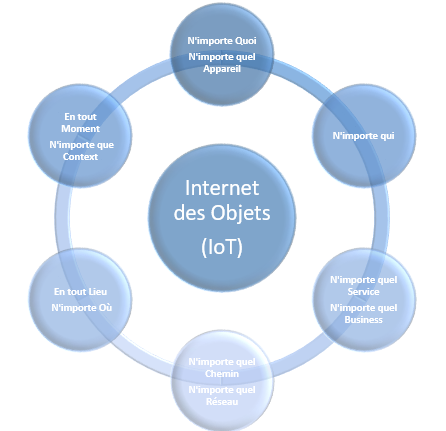
\includegraphics{IMAGES/ORIGINALS/Internet_des_Objets}
		\end{center}
		\caption{Internet des Objets}
	\end{figure}

L’Internet des Objets peut être déf{\kern0pt}ini également comme « des données et des appareils disponibles en permanence à travers l’internet » \cite{hu2016security}.\\
Un objet connecté est un objet possédant la capacité d’échanger des données avec d’autres entités physiques ou numériques.\\
À peu près n'importe quel objet physique peut être transformé en un appareil IoT s'il peut être connecté à Internet pour être contrôlé ou communiquer des informations avec le réseau indépendamment de l’action humaine.\\
Pour illustrer, prenons un exemple dans le domaine de l’habitat intelligent, aussi connu sous le nom de Smart Home. Imaginez que votre réfrigérateur devienne intelligent. Un réfrigérateur capable de vous dire en temps réel le type de denrées qu’il y a à l’intérieur et capable de passer commande pour vous quand vous avez besoin de vous réapprovisionner. Ce genre de réfrigérateur est un exemple typique d'objet connecté. La figure \ref{iot} illustre ce réseau d'objets connectés
	\begin{figure}[H]
		\begin{center}
			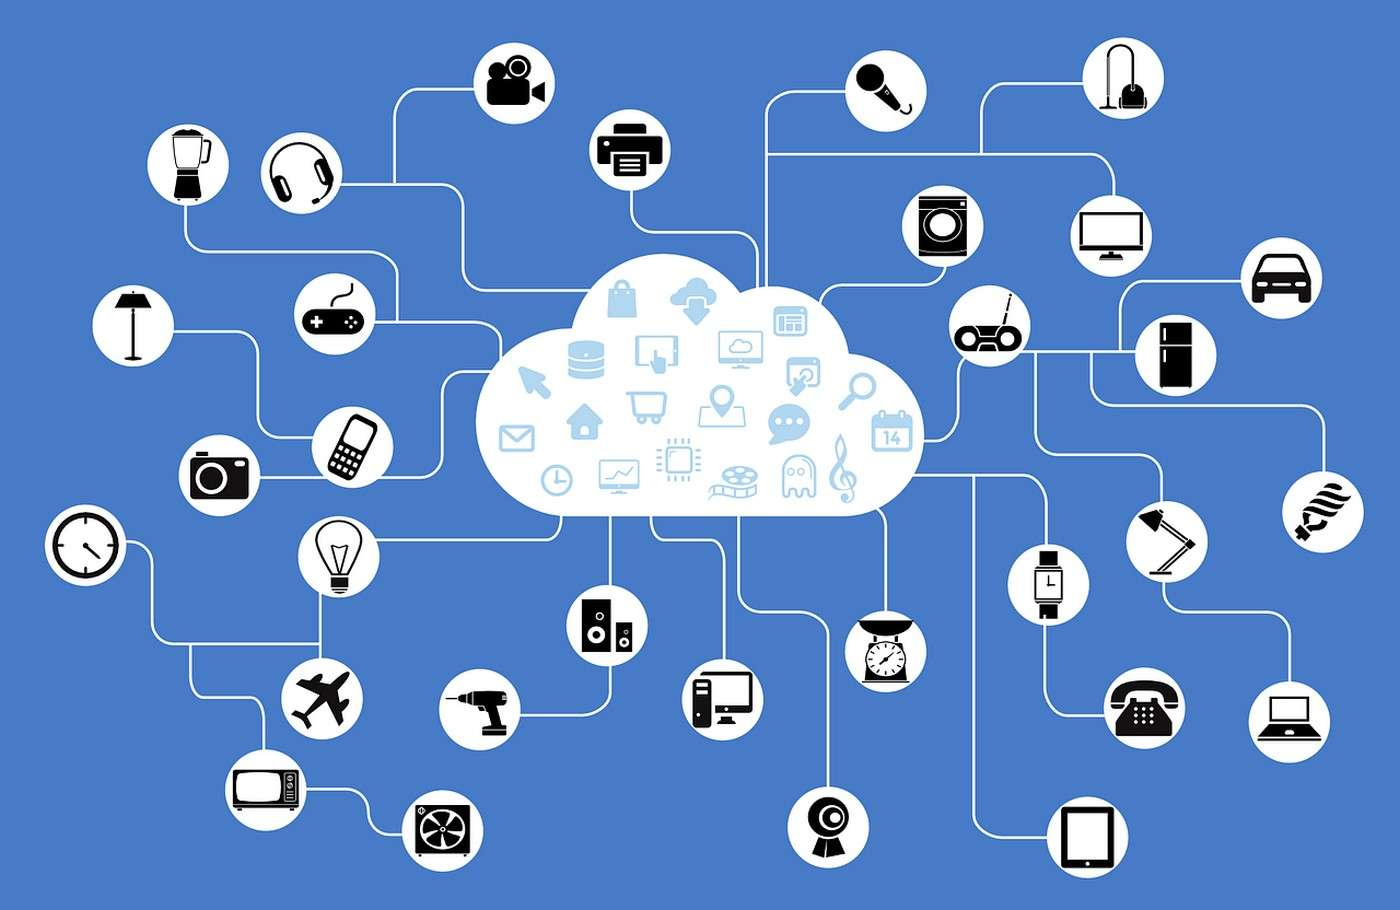
\includegraphics[width=16cm,height=14cm]{IMAGES/ORIGINALS/Internet_des_Objets_2}
		\end{center}
		\caption{Internet des Objets}
	\end{figure}	
	\section{Caractéristiques}
	Les caractéristiques fondamentales de l'IoT sont les suivantes \cite{patel2016iot}\cite{vermesan2014iot}\\
	\textbf{Inter connectivité}: en ce qui concerne l'IoT, tout peut être inter connecté avec l'infrastructure mondiale d'information et de communication.\\
	\textbf{Services liés aux objets}: l'IoT est capable de fournir des services liés aux objets dans les limites des objets, tels que la protection de la vie privée et la cohérence sémantique entre les objets physiques et les objets virtuels associés. Af{\kern0pt}in de fournir des services liés aux objets dans les contraintes des objets, les technologies du monde physique et du monde de l'information vont changer.\\
	\textbf{Hétérogénéité}: les appareils de l'IoT sont hétérogènes car basés sur dif{\kern0pt}férentes  plates-formes matérielles et réseaux. Ils peuvent interagir avec d'autres appareils ou plates-formes de services via dif{\kern0pt}férents réseaux.\\
\textbf{Changements dynamiques}: l'état des appareils change de manière dynamique, par exemple, le sommeil et le réveil, connectés et / ou déconnectés ainsi que le contexte des appareils, y compris l'emplacement et la vitesse. De plus, le nombre d'appareils peut changer dynamiquement.\\
	\textbf{Échelle énorme}: le nombre d'appareils qui doivent être gérés et qui communiquent entre eux sera au moins d'un ordre de grandeur supérieur à celui des appareils connectés à l'Internet actuel. Encore plus critique sera la gestion des données générées et leur interprétation à des f{\kern0pt}ins d'application. Cela concerne la sémantique des données, ainsi que la gestion ef{\kern0pt}f{\kern0pt}icace des données.\\
	\textbf{Sécurité}: à mesure que nous tirons profit de l'IoT, nous ne devons pas négliger la sécurité. En tant que créateurs et destinataires de l'IoT, nous devons concevoir des objets pour la sécurité. Cela comprend la sécurité de nos données personnelles et la sécurité de notre bien-être physique. Sécuriser les points de terminaison, les réseaux et les données se déplaçant sur tout cela signif{\kern0pt}ie créer un paradigme de sécurité qui évoluera.\\
	\textbf{Intelligence} : L'IoT est livré avec la combinaison d'algorithmes et de calcul, de logiciels et de matériel qui le rendent intelligent. Ce qui le rend encore plus intelligent, ce sont les données qu’il recueille à travers un capteur. L'intelligence ambiante dans l'IoT améliore ses capacités qui facilitent les choses pour répondre de manière intelligente à une situation particulière et les aide à ef{\kern0pt}fectuer des tâches spécif{\kern0pt}iques. Malgré toute la popularité des technologies intelligentes, l'intelligence dans l'IoT ne concerne que les moyens d'interaction entre les appareils, tandis que l'interaction utilisateur et appareil est obtenue par des méthodes d'entrée standard et une interface utilisateur graphique.\\
	\textbf{Connectivité}: la connectivité permet l'accessibilité et la compatibilité du réseau. L'accessibilité se fait sur un réseau tandis que la compatibilité of{\kern0pt}fre la capacité commune de consommer et de produire des données.
	\section{Architecture de l’IoT}	
	L’IoT devrait être capable d’interconnecter des milliards d’objets hétérogènes via le réseau internet, ainsi il est judicieux d’adopter une architecture flexible.\\	
Le modèle de base est une architecture à trois-couches comportant les couches Application, Réseau, et Perception. D’autres modèles ont été proposé récemment qui ajoutent plus d’abstraction aux architectures des objets connectés. La f{\kern0pt}igure ci-dessous illustre les dif{\kern0pt}férentes catégories de l’architecture IoT \cite{al2015iot}.
	\begin{figure}[H]
		\begin{center}
			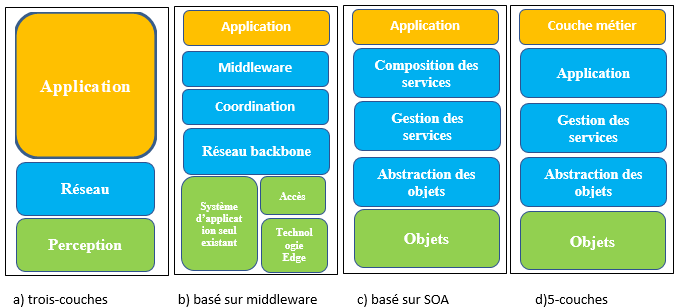
\includegraphics[width=\textwidth]{IMAGES/ORIGINALS/diverses_architectures_de_l'IoT}
		\end{center}
		\caption{Diverses architectures de l'IoT}
	\end{figure}
	\subsection{Architecture à trois couches}
	\subsubsection{Couche perception }
La première couche de l’IoT, les Objets (appareils) ou couche perception, est un organe sensoriel de l’IoT et représente les capteurs physiques de l’IoT qui essaie de recueillir et traiter les données. Un capteur de température permet de traduire l'amplitude de la température en une tension électrique. Cette couche comprend principalement des éléments avec des étiquettes RFID, capteurs, et autre terminaux. Elle détecte les données de l’environnement. Certains facteurs sont pris en charge par la couche physique tels que : ressource, hétérogénéité, déploiement, protocoles.
	\subsubsection{Couche réseau}
La couche réseau est chargée de récupérer les données collectées du capteur. L’échange des données se fait via cette couche. Ainsi, la couche réseau peut agréger les données dans sa propre base de données ou un stockage cloud.
	\subsubsection{Couche application}
La couche application ou la couche interface utilisateur contient les méthodes d’interaction avec les applications de l’utilisateur.
	\subsection{Architecture à cinq couches}
	\subsubsection{Couche Objets}
La première couche de l’IoT, les Objets (appareils) ou couche perception, représente les capteurs physiques de l’IoT qui essaie de recueillir et traiter les données. Cette couche comprend les capteurs et les actionneurs qui fonctionnent dif{\kern0pt}féremment. Un capteur de température permet de traduire l’amplitude de la température en une tension électrique. On a d’autres grandeur mesurable tels que pression, luminosité, position, vitesse. Quant aux actionneurs, ils permettent d’agir dans le monde physique en changeant son état. Un actionneur peut allumer un appareil à distance. La couche perception collecte les informations du capteur, numérise et transmet les données à la couche Abstraction Objet via un canal sécurisé.
	\subsubsection{Couche Abstraction Objet}
La couche Abstraction Objet transfert les données produit par la couche perception à la couche Gestion Service à travers des canaux sécurisés. Les données peuvent être transféré via des technologies variés tels que RFID, GSM(2G), UMTS(3G), LTE(4G), WI-FI, Bluetooth, Zigbee, etc. En plus, d’autres fonctions comme Cloud Computing et le traitement de gestion de données sont gérés par cette couche.
	\subsubsection{Couche Gestion des Services}
La couche Gestion des Services garantit la fourniture des services en fonction de la demande de l'utilisateur dans un environnement réseau hétérogène.
	\subsubsection{Couche Application}
La couche Application fournit les services demandés par les clients. Par exemple, la couche application peut fournir les mesures de température au client qui demande cette information.
Elle couvre dif{\kern0pt}férentes applications, à savoir: ville intelligente, transport intelligent, soins de santé, agriculture intelligente, maison intelligente, etc.
	\subsubsection{Couche Business}
La couche métier(gestion) est chargée de gérer l’ensemble des activités et des services comme les modèles métiers. Elle aide à construire un graphique, un organigramme, un modèle métier, une prise de décision etc. basé sur les données reçues de la couche Application.
	\section*{Domaines d’application}
Il existe une panoplie de domaines d’application extrêmement diverses pour les secteurs de l’internet des objets, du machine to machine et des objets connectés. Parmi ces principaux domaines, nous citons : la smart city, la domotique, les transports, la santé, l’industrie, l’agriculture.
	\begin{figure}[H]
		\begin{center}
			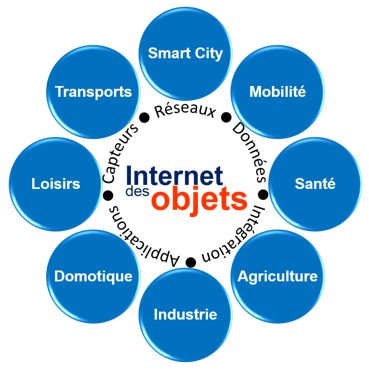
\includegraphics{IMAGES/ORIGINALS/Application_IoT}
		\end{center}
		\caption{Domaines d'application de l'IoT}
	\end{figure}
		\subsection*{ Smart city }
Dans les villes intelligentes, il améliore la qualité de vie des habitants en utilisant les nouvelles technologies pour accroître l’ef{\kern0pt}f{\kern0pt}icacité des services, optimiser l’éclairage, de maîtriser la consommation d’énergie et de réduire l’impact écologique des activités urbaines.
		\subsection*{Domotique }
		La domotique regroupe l’ensemble des technologies permettant l’automatisation des équipements d’un habitat. Elle vise à apporter des solutions techniques pour répondre aux besoins de confort (gestion d’énergie, optimisation de l’éclairage et du chauf{\kern0pt}fage), de sécurité(alarme) et de communication (commandes à distance) \cite{locqueneux2015domotique}.\\
		La domotique couvre trois domaines principaux :
		\begin{itemize}
			\item Confort de la vie quotidienne : l’IoT permettra aux propriétaires de villa de déclencher arrosage, fermeture des fenêtres ou tonte du gazon en fonction des informations transmises par les capteurs disposés dans le jardin.
			\item Assurer la protection des personnes et des biens par la prévention des risques d’accident (incendies, fuite de gaz, etc.).
			\item Faciliter les économies d’énergie grâce à la réaction maitrisée d’une maison intelligente.
		\end{itemize}
		\subsection*{Santé }
		Dans le domaine de la santé, l’internet des objets of{\kern0pt}frira une sécurité accrue à un patient dont un capteur est intégré sur le corps qui donne la possibilité d’être monitoré à distance.\\
Il peut informer un patient quand il est temps de prendre le médicament. En outre, cela pourrait éventuellement informer le médecin d’une situation d’urgence lui permettant ainsi de localiser le patient grâce à l’objet connecté
\subsection*{Transport }
		Des voitures connectées ou autonomes aux systèmes de transports intelligents, l’IoT pourra sauver des vies, réduire le traf{\kern0pt}ic et minimiser l’impact des véhicules sur l’environnement.
		
		\subsection*{Industrie }
		Dans le secteur industriel, le machine to machine peut augmenter énormément la productivité et la performance d’une usine. Par exemple, supposons un réseau de capteurs polyvalents qui suit à distance et pilote le fonctionnement des machines en leur donnant la possibilité de déclencher elles-mêmes un réapprovisionnement en matières premières.
		
		\subsection*{Agriculture :}
		L’internet des objets à un impact énorme sur le domaine de l’agriculture. Les éleveurs en bénéf{\kern0pt}icient en ef{\kern0pt}fectuant un suivi plus précis de l’alimentation, de la santé et de la sécurité du bétail. Ils peuvent aussi géolocaliser leur bétail en temps réel. Les agriculteurs peuvent aussi recueillir des données sur les engrais et les pesticides nécessaires à leurs cultures \cite{krigman2018agriculture}.
	
	\section{Enjeux et déf{\kern0pt}is de l’IoT}
	L’internet des objets soulève un nombre important de questions, mais le plus important porte certainement sur la sécurité. Beaucoup de produit connectés, dont certains que nous utilisons au quotidien af{\kern0pt}f{\kern0pt}ichent un réel manque de maturité impliquant de nouvelles préoccupation notamment autour de la conf{\kern0pt}identialité et la sécurité des données.\\
Mirai est un exemple type de cyberattaques résultant de menaces de sécurité liées à l’IoT.

\begin{table}[H]
	\begin{center}
	\begin{tabular}{|p{3cm}|p{10cm}|}
		\hline 
\textbf{Enjeux} & \textbf{Déf{\kern0pt}is} \\ 
		\hline 
Architecture & De nombreux chercheurs ont proposé diverses architectures non encore standardisé. \\ 
		\hline 
Sécurité & L’échange d’information entre des milliards d’objets connecté sur internet se fait via une connexion réseau sans f{\kern0pt}il. \\ 
		\hline 
Conf{\kern0pt}identialité & Les opérations d’accès aux prof{\kern0pt}ils entre objets sans interférences sont dif{\kern0pt}f{\kern0pt}iciles. \\ 
		\hline 
Intéroperabilité & Communication machine à machine (M2M), un déf{\kern0pt}i de l’IoT dû à la nécessité de gérer un grand nombre d’objets hétérogènes qui appartiennent à dif{\kern0pt}férentes plates-formes. \\ 
		\hline 
Disponibilité & La capacité à fournir des services à tout moment, n’importe où et n’importe quoi est un déf{\kern0pt}is. \\ 
		\hline 
Mobilité & L'utilisateur ou les appareils qui se connectent peuvent obtenir les services lors de leurs déplacements, ce qui constitue un déf{\kern0pt}i. \\ 
		\hline 
Scalabilité & La possibilité d'ajouter de nouveaux appareils qui n'af{\kern0pt}fecte pas la qualité de services existent est un déf{\kern0pt}i. \\ 
		\hline 
	\end{tabular} 
	\end{center}
	\caption{Enjeux et déf{\kern0pt}is de l'IoT}
\end{table}
	\section{Sécurité, conf{\kern0pt}identialité (privacy) en IoT}
L’IoT nécessite cinq phases, de la collecte des données, du stockage, du traitement, de la transmission des données à la livraison des données aux utilisateurs f{\kern0pt}inaux sur demande ou non \cite{hu2016security}. Les capteurs collectent dans de nombreux cas des données extrêmement sensible (personnelles). En ef{\kern0pt}fet les objets connectés produisent de grandes quantités de données à la phase de collecte de données et le traitement de cette masse de données implique de nouvelles préoccupations notamment autour de la conf{\kern0pt}identialité et la sécurité des données.
	\begin{figure}[H]
		\begin{center}
			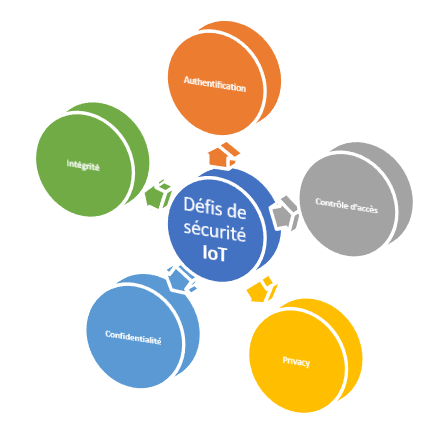
\includegraphics[width=\textwidth]{IMAGES/ORIGINALS/Défis_de_sécurité_IoT}
		\end{center}
		\caption{Déf{\kern0pt}is de sécurité IoT}
	\end{figure}

	\subsection{Sécurité pour l’IoT}
La sécurité est l’af{\kern0pt}faire de tous, elle concerne chacun de nous. Si vous achetez un verrou « intelligent » pour votre porte d’entrée, il est fort probable que vous allez vous faire pirater dans un premier temps puis cambrioler. L’IoT a des avantages et apporte tous celui d’internet à des éléments comme les thermostats et les ampoules par exemple mais sans oublier qu’il apporte également les problèmes d’internet. A présent que les gens ont leur réfrigérateurs, sonnettes, télévisions, ampoules, caméras de sécurité, haut-parleur connectés au Wi-Fi, presque tous les appareils de la maison peuvent être compromis ou rendu inutiles. En ef{\kern0pt}fet les objets connectés peuvent servir de point d’accès à votre réseau avec vos portables, votre PC, bref toute votre vie.\\

La menace qui pèse sur les appareils connectés à Internet ne vient pas uniquement du fait qu’ils sont connectés à Internet, mais aussi parce que les fabricants d’appareils n’ont pas toujours conçu leurs produits en privilégiant la sécurité. À mesure que l'IoT se répand largement, les cyberattaques risquent de devenir de plus en plus physiques (et pas simplement virtuelles) \cite{clearfield2013rethinkingsiot}. Les appareils contrôlés par ordinateur dans les automobiles, tels que les freins, les moteurs, les serrures, les klaxons, les systèmes de chauf{\kern0pt}fage et les tableaux de bord, se sont révélés vulnérables aux attaquants qui ont accès au réseau de bord \cite{andy2013hackers,boyle2010proof}. La possibilité qu'un intrus puisse démarrer à distance le chauf{\kern0pt}fage, régler le climatiseur, déverrouiller les portes, déployer des airbags pendant que vous conduisez sans accident ou tourner le volant d'une voiture en marche est en ef{\kern0pt}fet inquiétante, ef{\kern0pt}frayante.\\

Jusque-là l’essentiel des dommages subit par l’IoT a été causé par les botnets. En septembre 2016, une attaque a été mis en place par des centaines de milliers d’objets connecté piraté pour former un énorme botnet appelé Mirai. Ce malware a exploité des vulnérabilités (que les fabricants d’objet connecté ne prenaient pas en compte) dans plus de 600 000 appareils IoT pour créer une attaque massive par déni de service distribué (DDoS). Il avait pour objectif de dénoncer les risques de l’IoT.\\

En raison de la vulnérabilité du WPA2(protocole qui sécurise les échanges en Wi-Fi), tout ce qui est connecté à un réseau Wi-Fi risque d’être piraté \cite{kasperski201krack}. L'année suivante après Mirai, une attaque appelée KRACK acronyme de Key Reinstallation Attack (attaque de réinstallation de clé) a infecté presque tous les appareils connectés à Internet connectés au Wi-Fi. L'attaque était paralysante et dif{\kern0pt}f{\kern0pt}icile à résister, en partie parce que l'Internet des objets fonctionne sur de nombreux systèmes d'exploitation essentiellement dif{\kern0pt}férent. Lorsqu'un téléphone ou un ordinateur est touché par un virus, les fabricants de logiciels sont généralement prompts à émettre un correctif. Mais des choses comme les routeurs ou les sonnettes connectées à Internet ne sont pas mis à jour aussi régulièrement que les systèmes d’exploitation informatique pour se protéger contre les vulnérabilités, et beaucoup d'entre elles n'ont pas été construites avec le même type de protocoles de sécurité que les ordinateurs \cite{pardes2020iot}. C’est une réalité, l’IoT nous rend encore plus connecter et cette connexion de tous les instants vient avec son l’eau de risque qu’on ne peut pas ignorer. Les menaces virtuelles vont s’immiscer dans le monde physique, ce qui signif{\kern0pt}ie que le piratage des appareils peut avoir des conséquences dangereuses dans le monde réel.\\

L'IoT n'est pas encore arrivé à maturité et est extrêmement vulnérable à toutes sortes de menaces et d'attaques ou vol de données. Les systèmes de prévention ou de récupération utilisés dans le réseau traditionnel et Internet ne peuvent pas être utilisés dans l'IoT en raison de sa connectivité \cite{hu2016security}. Les raisons de sa vulnérabilité sont multiples \cite{atzori2010iot}. Primo, souvent ses composants passent la plupart du temps sans surveillance; et ainsi, il est facile de les attaquer physiquement. Secundo, la plupart des communications sont sans f{\kern0pt}il, ce qui rend l'écoute extrêmement simple. Enf{\kern0pt}in, la plupart des composants IoT sont caractérisés par de faibles capacités en termes à la fois d'énergie et de ressources informatiques (c'est particulièrement le cas pour les composants passifs) et, par conséquent, ils ne peuvent pas mettre en œuvre des schémas complexes prenant en charge la sécurité.\\
La sécurité des informations et du réseau doit être dotée de propriétés telles que, la conf{\kern0pt}identialité, l'intégrité, l'identif{\kern0pt}ication et la disponibilité. Plus précisément, les problèmes majeurs de l’IoT liés à la sécurité concernent l'authentif{\kern0pt}ication et l'intégrité des données \cite{atzori2010iot} : \\

	\begin{itemize}
		\item[$\bullet$] L'authentif{\kern0pt}ication est requise pour établir une connexion entre les appareils et l'échange de nombre de clés publiques et privées via le nœud pour empêcher le vol de données. L'authentif{\kern0pt}ication est dif{\kern0pt}f{\kern0pt}icile car elle nécessite généralement des infrastructures d'authentif{\kern0pt}ication et des serveurs appropriés qui atteignent leur objectif grâce à l'échange de messages appropriés avec d'autres nœuds. Dans l'IoT, de telles approches ne sont pas réalisables étant donné que les étiquettes RFID passives ne peuvent pas échanger trop de messages avec les serveurs d'authentif{\kern0pt}ication. Le même raisonnement s'applique (de manière moins restrictive) aux nœuds de capteur également.\\
		
		\item[$\bullet$] Les solutions d'intégrité des données doivent garantir qu'un adversaire ne peut pas modif{\kern0pt}ier les données de la transaction sans que le système détecte le changement. En d’autre terme, elles garantissent que les données qui sont arrivées au nœud récepteur sont inchangées et restent telles que transmises par la source (expéditeur). Un autre facteur critique qui influence l'intégrité des données est la robustesse et les capacités de tolérance aux pannes du système IoT. Les réseaux de capteurs, tels que les solutions RFID, sont également confrontés à d'autres problèmes qui limitent leur capacité à surmonter les problèmes d'intégrité, car bon nombre de leurs composants passent la plupart du temps sans être pris en charge, sans surveillance \cite{musonda2018iot}. Les données peuvent être modif{\kern0pt}iées par des attaquants pendant qu'elles sont stockées dans le nœud ou lorsqu'elles traversent le réseau \cite{karygiannis2007guidelines}. Pour protéger les données contre ces types d'attaque, les protections en lecture et en écriture ainsi que les méthodes d'authentif{\kern0pt}ication sont généralement des solutions courantes à ces problèmes. Les ressources trouvées dans les systèmes IoT courants ne prennent pas en charge les techniques cryptographiques (permettant de stocker, traiter et partager des données protégées sans que le contenu de l'information soit accessible à d'autres parties) typiques en raison des ressources limitées disponibles \cite{musonda2018iot}. L'intégrité de l'Internet des objets doit non seulement être protégée des sources externes mais également des processus internes, tels que l'intégrité des services.
	\end{itemize}
	\subsection{Conf{\kern0pt}identialité pour l’IoT}
Il y a ensuite la question de la conf{\kern0pt}identialité. La conf{\kern0pt}identialité des données est une condition pour que les données ne soient disponibles que pour les utilisateurs autorisés. Elle consiste à garder les données privées plutôt que de les autoriser à être disponibles dans le domaine public.\\
L’IoT représente un environnement dans lequel la vie privée des individus est fortement menacée. Si des caméras et des microphones sont installés autour de votre maison, ils vous regardent et vous écoutent. Tout dans l'internet des objets collecte des données et toutes ces données sont d’une valeur inestimable. Ainsi, lorsque les entreprises gagneront de l'argent en vous vendant des objets connectés intelligents en premier lieu, leur modèle commercial IoT implique probablement la vente d'au moins certaines de ces données également. Ce qui arrive à ces données est une question de conf{\kern0pt}identialité d'une importance vitale. Toutes les entreprises de maisons intelligentes ne construisent pas leur modèle commercial autour de la collecte et de la vente de vos données, mais certaines le font \cite{ranger2020iot}.\\

De nombreux appareils de dernière génération dans nos maisons sont équipés d'une connectivité qui permet une grande commodité, mais cet avantage a un prix (des risques potentiels d'espionnage et de sécurité). En janvier 2014, Forbes a répertorié de nombreux appareils connectés à Internet tels que des téléviseurs, des appareils de cuisine, des modems(et ISP), des, des caméras, des thermostats(chauf{\kern0pt}fage et climatisation), et des équipements de buanderie qui peuvent déjà « espionner des personnes dans leur propre maison » \cite{steinberg2014spying}. Cela signif{\kern0pt}ie que les détails les plus f{\kern0pt}ins de votre vie personnelle, tels que exposés par votre réfrigérateur intelligent, votre télévision intelligent ou votre haut-parleur intelligent, peuvent être recueillis et vendus à quelqu'un d'autre ou pour faire du chantage. Google et Apple ont tous deux admis, l'an dernier, que les enregistrements capturés par leurs haut-parleurs intelligents étaient examinés par des entrepreneurs, y compris des extraits audio maladroits et intimes.\\
La sécurisation des échanges de données est nécessaire pour éviter de perdre ou de compromettre la conf{\kern0pt}identialité.


	\section{Conclusion}
L’IoT est un concept en évolution constante dont l’objectif est d’étendre le réseau internet en interconnectant les objets connectés, ainsi ef{\kern0pt}fectué des échanges de données aux objets du monde physique. Ces objets connectés à internet peuvent prendre la forme de n’importe quel objet du quotidien.\\
Le terme \og Internet des Objets \fg{} a été inventé en 1999, initialement pour promouvoir la technologie RFID. Il existe plusieurs architectures de l’IoT tels que l’architecture basé trois-couches, basé sur middleware, basé sur SOA et basé cinq-couches.\\
Le résultat attendu des objets connectés est de s’adapter non seulement à nos besoins mais aussi à notre environnement.\\
Tout appareil connecté à Internet présente un risque élevé, et les appareils IoT ne font pas exception. L’IoT peut être vu comme « Interconnections of Threats » c’est-à-dire interconnexions des menaces dû à l’extension du réseau internet. La sécurité et la conf{\kern0pt}identialité des données sont de grands déf{\kern0pt}is dans l’IoT. Lors de la transmission transparente des données, il est important de se cacher des appareils d'observation sur Internet qui sont susceptibles de nous espionner.\\
Dans le prochain chapitre, nous allons aborder les notions de base de la sécurité informatique.
	
	

\chapter{Sécurité informatique et Cybersécurité} 
\minitoc
\thispagestyle{empty}
\newpage
\section{Introduction : }
%\parindent=0.2cm 

Dans un monde de plus en plus connecté où les progrès technologiques avancent à grande vitesse, où les gens, les entreprises, les organismes, les pays et même les objets sont de plus en plus connectés.
Dans un tel monde, il est absolument essentiel d'assurer une cybersécurité efficace. Tant que l'utilisation des TIC progressent, les risques augmenteront aussi. Il s'agit donc de répondre à des défis et des cybermenaces qui ne cessent d'évoluer, ce qui exige que tous les acteurs soient au courant des facteurs de risque, qu'ils disposent des capacités nécessaires et qu'ils prennent les mesures appropriées en matière de prévention et de résolution. Pour garantir un cyberespace sûr, résilient et sécurisé, les pays doivent explorer la réalité complexe et multisectorielle de la sécurité ce qui soulève des questions stratégiques, techniques, juridiques, politique, et qui suppose l'établissement d'une collaboration multisectorielle et internationale \cite{securite}.\\

Aujourd’hui notre mode de vie ultra connecté ne peut se passer des objets connectes et comme une connexion à un réseau rend possible une intrusion. Le fait d’interconnecter des objets augmentent d’autant plus la surface d’attaque aux cyber attaquants nous rendant ainsi beaucoup plus vulnérables. Cette multiplicité d’objets, de connexions, et de règlementation fait qu’aujourd’hui qu’il est difficile d’appliquer un seul modèle de sécurité. Le cyber espace est donc un monde à hauts risques d’attaques \cite{dangercyberespace}. Le mot anglais « Security » signifie une résistance à une malveillance, se traduit en français par « sûreté », alors que le mot « safety » signifie une résistance à une panne \cite{ref4ex}.\\

La sécurité informatique est l’ensemble des moyens techniques, organisationnels, juridiques et humains nécessaires mis en oeuvre pour réduire la vulnérabilité d’un système contre les menaces accidentelles ou intentionnelles. C’est une branche de la technologie de l’information qui étudie et met en oeuvre les menaces et les vulnérabilités des systèmes informatiques.\\
La cybersécurité assure la protection du cyberespace contre les cybers menaces. Le terme cybersécurité n’est pas synonyme de sécurité informatique\cite{ref1} . La cybersécurité s’applique aux systèmes interconnectés, du fait que l’information numérique à protéger voyage à travers eux et y réside en eux tant disque la sécurité informatique s'occupe des systèmes informatisés liés ou non à internet ou à des réseaux\cite{ref1e2}.
\section{Les objectifs de sécurité informatique : }
La notion de sécurité d’un système informatique s’exprime généralement en termes de disponibilité (D), d’intégrité (I) et de confidentialité (C)\cite{ref4}. Ces critères (dits critères DIC) sont les objectifs de sécurité de base dont leurs mises en oeuvre permettent d’atteindre un certain niveau de sécurité. En plus de ces fonctions s’ajoutent d’autres services de sécurité complémentaires pour confirmer la véracité ou l’authenticité d’une action ou d’une ressource (notion d’authentification) ou encore pour prouver l’existence d’une action à des fins de non-répudiation ou d’imputabilité, ou de traçabilité.\\
\cia
\subsection{La confidentialité : }
La confidentialité consiste à rendre l'information inintelligibles aux acteurs illégitimes d’une transaction ou d’une communication. Elle garantit l’anonymat des données en limitant leurs accès par le chiffrement et l’authentification.\\
La confidentialité assure que seules les personnes autorisées peuvent accéder à l’information. Les politiques d’entreprise devront limiter l’accès à l’information au personnel autorisé et garantir que seules ces personnes autorisées consultent ces données. Les données peuvent être compartimentées selon le niveau de sécurité ou de
sensibilité de l’information.\\
Par ailleurs, les employés doivent suivre une formation pour comprendre les bonnes pratiques en matière de protection des informations sensibles pour se protéger et pour protéger l’entreprise contre les attaques. Il existe deux méthodes complémentaires permettant d’assurer la confidentialité :
\begin{itemize}[label=\textbullet]
	\item Limiter et contrôler l’accès aux données afin que seules les personnes habilitées à les lire ou à les modifier puissent le faire.
	\item Rendre inintelligibles les données en les chiffrant de telle sorte que les personnes qui ne sont pas autorisées à les déchiffrer ne puissent les utiliser. Cette tache est réalisée en utilisant le chiffrement (cryptographie).
\end{itemize}
\subsection{L’intégrité :}
Vérifier l’intégrité des données consiste à déterminer si les données n'ont pas été altérées durant la communication. L’intégrité représente l’exactitude, la cohérence et la fiabilité des données pendant tout leur cycle de vie. Le critère d’intégrité des ressources physiques et logiques (équipements, données, traitements, transactions, services) assure qu’elles demeurent intactes, qu’elles n’ont pas été détruites ou modifiées à l’insu de leurs propriétaires tant de manière intentionnelle, qu’accidentelle.\\

Préserver l’intégrité des ressources et s’assurer que des ressources sont intègres sont l’objet de mesures de sécurité. Ainsi, se prémunir contre l’altération des données et avoir la certitude qu’elles n’ont pas été modifiées collabore à la qualité des prises de décision basées sur celles-ci. Si en télécommunication, l’intégrité des données relève essentiellement de problématiques \cite{ref4}liées au transfert de données, elle dépend également des aspects purement informatiques de traitement de l’information (logiciels d’application, systèmes d’exploitation, environnements d’exécution, procédures de sauvegarde, de reprise et de restauration des données). L’intégrité des données est mise en oeuvre par des mécanismes cryptographiques et les signatures numériques pour s’assurer que les données n’ont pas été victimes d’écoute ou d’altération lors de leur transfert par des cyberattaques
\subsection{La Disponibilité :}
La disponibilité d’une ressource est relative à la période de temps pendant laquelle le service qu’elle offre est opérationnel. Elle garantit la continuité à l’accès à un service ou à des ressources. Le volume potentiel de travail susceptible d’être pris en charge durant la période de disponibilité d’un service détermine la capacité d’une ressource à être utilisée. Il ne suffit pas qu’une ressource soit disponible, elle doit pouvoir être utilisable avec des temps de réponse acceptables. Sa disponibilité est indissociable de sa capacité à être accessible par l’ensemble des ayants droit (notion d’accessibilité).\\

La disponibilité des services, systèmes et données est obtenue par une maintenance des équipements, la réparation des matériels, la mise à jour des systèmes d’exploitation et des logiciels, la création de sauvegardes ainsi que l’utilisation d’équipements ou de service de sécurité. Les attaques de types DoS et DDOS  peuvent causer l’indisponibilité d’un service ou d’une ressource. Celles-ci, sont possibles si les procédures de sauvegarde et de restitution ainsi que les supports de mémorisation associés ne sont pas gérées correctement ou s’il y a malveillance. Une politique de sauvegarde et des systèmes de détection d’attaques de types DDOS doivent être mis en oeuvre pour éviter le risque d’indisponibilité d’un service ou d’une ressource.
\subsection{La traçabilité : }
L’enregistrement des activités permettent la traçabilité des événements et leur analyse. Garder la mémoire des actions survenues permet notamment de reconstituer et de comprendre ce qui s’est passé lors d’incidents afin d’améliorer la sécurité, d’éviter que des erreurs ne se répètent ou d’identifier des fautifs. Cela autorise par exemple d’analyser le comportement du système et des utilisateurs à des fins d’optimisation, de gestion des incidents et des performances ou encore d’audit.\\
L’enregistrement des actions et événements permet également d’enrichir les bases de données qui permettent de développer des applications de surveillance, de détection et de réaction aux incidents, en particulier à l’aide des techniques issues de l’intelligence artificielle.
\subsection{L’authentification et l’identification :}
L'identification consiste à attribuer une identité unique à un utilisateur. Elle permet de répondre à la question : Qui êtes-vous ?\cite{ref5}. Pour se faire l'utilisateur utilise un identifiant unique qu’on nomme Compte d'accès (Nom d'utilisateur ou Login en anglais). L’authentification consiste à assurer la véracité de l'identité d'un utilisateur. Elle permet de répondre à la question : êtes-vous réellement cette personne ? \cite{ref5} Pour se faire l’utilisateur utilise un authentifiant ou code secret (mot de passe ou password en anglais) dont lui seul à la connaissance.\\
L’identification et l’authentification des ressources et des utilisateurs permettent d’associer la réalisation d’une action à une entité qui pourra en être tenue responsable et éventuellement en rendre compte. Un contrôle d'accès permet l'accès à des ressources uniquement aux personnes autorisées à travers un mot de passe crypté.
\authenti
\subsection{La non-répudiation et l’imputabilité : }
La non-répudiation de l'information est la garantie qu'aucun des correspondants ne pourra nier une transaction, c'est-à-dire de garantir à chacun des correspondants que son partenaire est bien celui qu’il prête être en d’autres termes assurer la preuve d’origine ou de destination de message.\\
L’imputabilitéest la possibilité d’attribuer la responsabilité d’une infraction à un individu. Elle peut être réalisée par un ensemble de mesures garantissant l’enregistrement fiable d’informations pertinentes relatives à un événement. La non-répudiation et l’imputabilité sont assurer en utilisant les algorithmes de chiffrement asymétriques.
\section{Application de la sécurité informatique : }
La sécurité contient une variété de contextes et dépends du domaine d’application. On distingue 6 catégories de sécurité en fonction du domaine d’application  :
\begin{itemize}[label=\textbullet]
\item \textbf{Sécurité matérielle physique et environnementale};
\item \textbf{Sécurité logique et applicative};
\item \textbf{Sécurité de l’information} ;
\item \textbf{Sécurité de l’exploitation} ;
\item \textbf{Sécurité des réseaux };
\item \textbf{Cybersécurité}.
\end{itemize}
\imageAPS
\subsection{La cybersécurité :}
Le mot Cybernétique vient du grec « kuberneïn » qui signifie diriger ou gouverner, terme repris en 1948 par le mathématicien Norbert Wiener ancien professeur du Massachusetts Institute de Technologie (MIT) qui l’a publié pour la première fois dans son ouvrage intitulé Cybernetics, or Control and Communication in the Animal and the Machine\cite{cybernetics}.\\
Plusieurs décennies plus tard l’auteur de science-fiction William Gibson utilise le terme de cyberespace dans son roman le Neuromanien. Il s’agit d’une trilogie qui a pour personnage central un voleur de données. Celui-ci est à mesure d’établir des connexions entre son esprit et un réseau mondial liant des ordinateurs entre eux \cite{neuromacer}.\\
Au fuir du temps le préfixe \textit{cyber} va participer ainsi à la construction de nouveaux mots lui donnant une nouvelle définition. Cyber est un préfixe servant de créer de mots relatifs à l’utilisation d’internet et à cette société de l’information qui a vu le jour à la fin du XXème. Aujourd’hui il y a plus de 40 mots débutants par Cyber dont : Cybersécurité, cybernétique, cyberespace, cybercafé, cybercrime, cyberattaque, cyberdéfense, cyberguerre, cyberterroriste, cybermonde etc.\\Avec l’utilisation extensif d’Internet des objets générant de nouveaux types de menaces dont seule la cybersécurité peut y faire face.\\
La cybersécurité assure la protection du cyberespace contre les cybers attaques. Elle concerne la sécurité des systèmes accessibles via le cyberespace(internet)et englobe la sécurité de l’information, la sécurité des réseaux et des environnements connectés. Le cyberespace est un espace virtuel relatif à notre espace naturel en d’autres termes un ensemble d’infrastructures numériques, de données et services misent en réseaux mais contrairement à la terre, à la mer, à l’air et à l’espace-extra atmosphérique, le cyberespace est une pure création de l’être humain qui ne relève pas de la nature \cite{ref4}. Le terme cybersécurité est large et englobe chaque élément, de la sécurité de l’ordinateur à la reprise de l’activité après sinistre et la formation des utilisateurs \cite{ref8}
\subsection{La sécurité des réseau : }
La sécurité d’un réseau consiste à protéger un réseau informatique contre les intrus, qu'il s'agisse d'attaques ciblés ou de logiciels malveillants en d’autres termes protéger les équipements, les applications et les données du réseau contre les cybers attaques. Elle utilise plusieurs services et protocoles de défense allant de la couche physique à la couche application. Pour se faire plusieurs approches sont utilisés dans le modèle TCP/IP comme décrit ci-dessous :
\begin{itemize}[label=\textbullet]
\item Couche transport (protocoles TLS/SSL, SSH),
\item Couche internet (protocole IP Sec);
\end{itemize}
\subsubsection{Protocoles TLS/SSL :}
\textbf{TLS} de l’acronyme \textbf{T}ransport \textbf{L}ayer \textbf{S}ecurity et \textbf{SSL} de l’acronyme \textbf{S}ecure \textbf{S}ocket \textbf{L}ayer, sont des protocoles de chiffrement qui garantissent la sécurité des échanges de données via un réseau informatique. Ils sont largement utilisés pour la sécurisation des communications sur internet.\\
Ils utilisent les techniques de chiffrements asymétriques et des algorithmes de cryptage comme RSA, ECC, pour assurer la confidentialité, l’intégrité des données ainsi que l’authentification et l’identification des utilisateurs.
\subsubsection{Le protocole IPSec :}
IP Sec pour Internet Protocol Security est une suite de protocoles normalisés par L’Internet Engineering Task Force (IETF) qui fournit des services de sécurisations des données dans un réseau IP au niveau de la couche réseau. Fondé dans le but d’assurer la sécurité du protocole IPv6 et a été réadapter par la suite au protocole IPv4. Il assure les critères de confidentialité, d’authentification et d’intégrité des données échangées à travers un réseau IP ainsi qu’à la création de réseau privé virtuel (VPN).\\
L’IPSec peut fonctionner en deux : mode transport et mode tunnel. Le mode transport est utilisé pour les communications de bout en bout (Host to Host). Le mode tunnel est utilisé pour les configurations passerelle à passerelle ou passerelle à hôte (Gate-to-Gate ou host-to-Gate)\cite{ref9}.\\

En plus de ces protocoles il existe plusieurs moyens classiques pour protéger un réseau informatique dont : les firewalls, la segmentation du réseau, les anti-virus et anti-malwares, les contrôles d’accès réseaux, les zones démilitarisés (DMZ) dont nous détaillerons dans la section mécanismes de sécurité.
\subsection{La sécurité logique et applicative :}
La sécurité des applications se concentre sur la protection des logiciels contre les menaces. Une application compromise pourrait fournir un accès aux données qu'elle est destinée à protéger. Une sécurité réussie commence au stade de la conception, bien avant le déploiement d'un programme ou d'un périphérique.\\
La sécurité logique fait référence à la réalisation de mécanismes de sécurité par logiciel contribuant au bon fonctionnement des programmes, des services offerts et à la protection des données. Elle s’appuie généralement sur :
\begin{itemize}
\item La qualité des développements et l’implémentation des logiciels et des tests de sécurité ;
\item Une mise en oeuvre adéquate de la cryptographie pour assurer intégrité et confidentialité ;
\item Des procédures de contrôle d’accès logique, d’authentification ;
\item Des procédures de détection de logiciels malveillants, de détection d’intrusions et d’incidents ;
\item La sécurité applicative comprend le développement pertinent de solutions logicielles (ingénierie du logiciel, qualité du logiciel) ainsi que leur intégration et exécution harmonieuses dans des environnements opérationnels.
\end{itemize}
\subsection{La sécurité des informations : }
La sécurité de l'information est un ensemble de stratégies de gestion et politiques de sécurités visant à protéger, détecter, recenser et contrer les menaces ciblant les données.  Elle vise à protéger des données et s'applique à tous les aspects de la sûreté, l'intégrité, la disponibilité et la confidentialité, la garantie, et la protection d'une donnée ou d'une information quelle que soit sa forme, tant en stockage qu'en transit \cite{ref8}. Une donnée est la représentation d’une information.

Le système d’information étant le maillon de l’entreprise, l’information qui y transite doit être impérativement protéger contre le vol, la destruction et la falsification d’information pouvant causer d'énorme pertes à l’entreprise. Une classification des données permet de qualifier leur degré de sensibilité (normale, confidentielle, etc.) et de les protéger en fonction de ce dernier
\subsection{La sécurité d'exploitation : }
La sécurité de l'exploitation est un ensemble de stratégies de gestion et de politiques de sécurités visant à assurer le bon fonctionnement opérationnel des systèmes informatiques. Cela comprend la mise en place d'outils et de procédures relatifs aux méthodologies d'exploitation, de maintenance, de test, de diagnostic, de gestion des performances, de gestion des changements et des mises à jour\cite{ref4}. Elle s'appuie sur les différents mécanismes et services de sécurités suivants :
\begin{itemize}[label=\textbullet]
\item Une gestion des systèmes d’exploitation, des configurations et des mises à jour ;
\item Gestion des incidents et suivi jusqu’à leur résolution ;
\item Une politique de sauvegarde, de secours, de continuité et de tests;
\item Gestion des contrats de maintenance ;
\item Une analyse des fichiers de journalisation et de comptabilité 
\end{itemize}
\section{Anatomie d'une attaque :}
Une attaque informatique est l'exploitation d'une faille de sécurité d'un système dans le but de le violer et de l'utiliser pour réaliser des actions malveillantes. Une attaque peut se faire par un individu ou un groupe d'individus, contre l'ordinateur d'un individu ou d'un groupe de personnes morale ou physique. Elle se déroule en générale en cinq actions fréquemment appelés les 5 P  \cite{ref5p} : Probe, Penetrate, Persist, Propagate, Paralyze.
\begin{itemize}
\item\textbf{Probe} (phase d'analyse): consiste à l'identification de la cible. Pour se faire l'attaquant se sert des outils comme whois, Arin, DNS lookup pour collecter le maximun d'information sur la cible en vue d'identifier d'éventuelles vulnérabilités.
\item\textbf{Penetrate} (phase de pénétration) : consiste à l'utilisation des informations et vulnérabilités récoltées pour pénétrer un réseau.
\item\textbf{Persist} (persister) : une fois le réseau infiltré, le pirate procédera à la création de droit administrateur en vue d y revenir facilement. Pour cela, il installera par exemple des back doors ou cheval de Troie en français.
\item\textbf{Propagate} (propager) : le réseau  infiltré, l'accès à un compte administrateur, Le pirate pourra ensuite  explorer le réseau afin de trouver de nouvelles cibles sur le réseau local. 
\item\textbf{Paralyze} (paralyser) : cette phase est la plus dangereuse. Elle est l'étape finale qui consiste à l'exécution  de l'attaque. pour cela le pirate peut utiliser le serveur ou la machine infiltrée pour attaquer une autre machine, détruire des données ou encore endommager le système d’exploitation dans le but de le nuire
\end{itemize}
\section{Les types de menaces et d’attaques : }
Une menace est une cause potentielle d’incident, qui peut provoquer un dommage sur un système et ayant un impact sur ses fonctionnalités, son intégrité ou sa disponibilité. Une cybermenace est une menace qui s’exprime via le cyberespace, qui peut toucher tout système connecté à Internet dont sa concrétisation par une cyberattaque, peut affecter le bon fonctionnement des ordinateurs, des réseaux de télécommunication et de tous les services et activités humaines qui en dépendent\cite{cybermenace}. Les cybermenaces sont le plus souvent associées à l’usage malveillant des technologies Internet et à la cybercriminalité. De nombreuses cyberattaques existent, elles recouvrent des réalités diverses en fonction des cibles touchées, de leurs impacts, finalités, origines et auteurs.
\subsection{La cybercriminalité : }
Selon Colin ROSE \cite{ref10} La cybercriminalité est la troisième grande menace pour les grandes puissances, après les armes chimiques, bactériologiques, et nucléaires. Le cout global de la cybercriminalité est estimé à 6000 milliards de dollars et triplera le nombre d’emplois non pourvu en cybersécurité d’ici 2021 \cite{ref1112}.\\
\textbf{La cybercriminalité} est toute infraction impliquant l’utilisation des technologies informatiques. Elle comprend des acteurs uniques ou des groupes ciblant des systèmes à des fins de gain financier ou de perturbation. Malgré que les entreprises et les forces de l’ordre tentent de s’attaquer au problème croissant, le nombre de cybercriminels continue de croître, profitant de l’anonymat d’Internet.\\
La cybercriminalité se divise en trois grandes catégories \cite{ref1112} : la cybercriminalité individuelle, la cybercriminalité contre la propriété et la cybercriminalité gouvernementale 
\begin{description}
\item[La cybercriminalité individuelle] est une catégorie de cybercriminalité dont le criminel utilise des informations et programmes malveillants pour arriver dans le but de nuire à un individu.
\item[La cybercriminalité contre la propriété] est la catégorie de cybercriminalité dont le criminel s’usurpe (vol d’identité) de l’identité d’une personne. Une fois le criminel possède les informations personnelles volées il procède à des achats, des élévations de privilèges afin d’accéder à des informations confidentielles ou au chantage.
\item[La cybercriminalité gouvernementale] est l’infraction la plus grave qui consiste à un crime contre le gouvernement, par exemple le piratage de sites web gouvernementaux ou de la diffusion de propagande. Ces genres de cyberattaques sont menés par des terroristes ou dans le cadre d’une cyberguerre entre nations.
\end{description}
\subsection{DDoS (Distributed Denied of Service) : }
Le DDoS est une attaque informatique ayant pour but de rendre indisponible un service, d'empêcher les utilisateurs légitimes d'un service de l'utiliser. La ressource peut être une seule machine (comme un serveur), un groupe de machines(comme un pool de serveurs dédiés), voire un réseau. Le DDoS est actuellement l’une des attaques la plus dangereuse pour les états, les entreprises causant beaucoup de perte d’argent et même en vie humaine si elle est bien structurée et visant des infrastructures critiques\cite{refados}. Voilà pourquoi nous avons fait le choix de nous focaliser sur ce type d’attaque. Le chapitre suivant est consacré entièrement à l’attaque DDoS.
\subsection{L'ingénierie sociale : }
L’ingénierie sociale est un ensemble des techniques de manipulation psychologique ou d’exploitation comportementale d’un individu, ou d’un groupe d’individus, par des personnes malfaisantes dont le but est l’incitation à amoindrir, contourner ou supprimer les mesures de sécurité d’un système par ce ou ces individus \cite{ref13}.\\
L’ingénierie sociale se sert en général des comportements ou de la personnalité particulière de leurs cibles tels que la naïveté, les émotions personnelles, les centres d’intérêt, L’adresses e-mail, la serviabilité, la confiance, le respect, la fierté, la reconnaissance dans le but de s’emparer de leurs accès informatiques. Elle procède comme suite : 
\begin{itemize}
	\item Collecte d’information,
	\item Etablissement de relations,
	\item Exploitations des vulnérabilités identifiées,
	\item Et ensuite l’exécution.
\end{itemize}
Les types d’attaques d’ingénierie sociale les plus utilisées sont : l’hameçonnage, le vishing, etc.
\subsubsection{L’Hameçonnage : }
L’hameçonnage ou phishing en anglais est l’une les plus courantes des attaques d’ingénierie sociale. C’est un courriel frauduleux ou un faux site conçu en usurpant l’identité d’un individu ou d’une organisation pour inciter leurs cibles à révéler des informations privées (nom d’utilisateur, mots de passe, information de cartes de crédit, etc.) ou télécharger des logiciels malveillants.\\

Les courriels d'hameçonnage reposent sur des tactiques de peur, comme des courriels urgents de votre banque ou d'une autre institution financière, ou de votre patron, comme des offres de produits bon marché ou difficiles à trouver ou votre sens du devoir envers votre patron. Ça pourrait être aussi un faux site web contrôler par l’attaquant, usurpant d’un site officiel incitants les utilisateurs à fournir leurs informations personnelles.
\subsubsection{Le vishing : }
Le vishing ou attaque par téléphone est la version téléphonique de l’hameçonnage et la plus facile à mettre en oeuvre, c’est une technique frauduleuse utiliser par les pirates pour récupérer des informations (généralement bancaires) auprès d’utilisateurs de téléphone portable.\\

Les hackers qui utilisent cette technique préparent soigneusement leur personnage et leur discours, au préalable et ensuite appeler leur cible dans le but d’obtenir des renseignements le plus rapidement possible. Certains pour parfaire leur crédibilité, utilisent un magnétophone ou une cassette préalablement enregistrée de bruits de bureau, ou encore utiliser un matériel qui change le timbre de la voix pour imiter celle d'une secrétaire ou d’un patron.

\subsection{Attaque par brute force et par dictionnaire : }
L’objectif de ces attaques est généralement le même; deviner le bon mot de passe ou de décrypter un texte en utilisant des tentatives, des techniques et des logiciels de décryptage. Elle se base sur la philosophie \textit{n’importe quel mot de passe est crackable ce n’est qu’une question de temps.}\\

\textbf{L’attaque par force brute} consiste à tester de façon exhaustive toutes les combinaisons possibles de caractères (alphanumérique, symbole) de manière à trouver un mot de passe valide. Elle se base sur le fait que n’importe quel mot de passe est crackable ce n’est qu’une question de temps.\\

\textbf{L’attaque par dictionnaire} consiste à cracker un mot de passe en se basant sur document répertoriant des mots courants, des prénoms, des noms d’animaux ou des objets etc.
Les outils d'attaque par force brute peuvent demander des heures, voire même des jours ou des années, de calcul même avec des machines équipées de processeurs puissants. Ainsi, une alternative consiste à effectuer une « attaque par dictionnaire » souvent vue comme un complément de l’attaque par brute fore. En effet, la plupart du temps les utilisateurs choisissent des mots de passe ayant une signification réelle. Avec ce type d'attaques, un tel mot de passe peut-être craquer en quelques minutes
\subsection{Attaque par Homme du milieu :}
Attaque par homme du milieu (HDM) ou man-in-the-middle en anglais (MITM) est une attaque par laquelle un attaquant accède aux communications entre deux noeuds légitimes, sans qu’aucune de ces deux noeuds ne s’en rende compte. L’attaquant peut lire le contenu de la communication, parfois les modifier.
\imgMiM
Pour se faire l’attaquant passe généralement par une connexion internet et doit donc être capable de recevoir les messages (les décrypter s’ils sont chiffrés) des deux parties et d'envoyer des réponses à une partie en se faisant passer pour l'autre \cite{ref14}.

\subsection{Logiciels Malveillants (Malware) :}
Un logiciel malveillant est un type de logiciel conçu pour obtenir un accès non autorisé ou pour endommager un ordinateur. Il comporte un ensemble de programmes conçus par un pirate pour être implantés dans un ordinateur à l’insu de l’utilisateur. I1 regroupe les virus, vers, spywares, keyloggers, chevaux de Troie, backdoors etc.
\subsubsection{Les virus : }
Un virus informatique est un programme ou un code malveillant qui est chargé dans votre ordinateur à votre insu sans votre autorisation. Certains virus sont seulement désagréables, mais la plupart sont destructeurs et sont conçus pour infecter les systèmes vulnérables et en prendre le contrôle.\\

Les virus sont généralement attachés à un fichier exécutable ou un document Word. Ils se propagent souvent via le partage de fichiers en P2P, de sites Internet infectés et le téléchargement
de pièces jointes. A l’interaction avec ces fichiers infectés par exemple le clic sur un fichier, l’ouverture d’un fichier ou à l’exécution d’un programme, le virus s’exécute automatiquement et s’installe dans l’ordinateur de la victime. Une fois qu’un virus pénétré dans votre système, il restera en dormance jusqu’à l’activation du programme ou du fichier hôte infecté, qui à son tour activera le virus et lui permettra de s’exécuter et de se reproduire sur votre système \cite{ref13}.
\subsubsection{Chevaux de Troie : }
Le cheval de Troie est un logiciel qui ne se reproduit pas et permet d’ouvrir une « porte » sur l’ordinateur de la victime pour en prendre ultérieurement le contrôle ou activer à distance des programmes nocifs appelés « malwares ».\\ 

Encore appelé « Trojan Horse » en anglais, ce type de logiciel n’est rien d’autre que le véhicule, celui qui fait entrer le programme malveillant à l’intérieur de la machine. Il n’est pas nuisible en lui-même car il n’exécute aucune action, si ce n’est de permettre l’installation du vrai programme malveillant.
Très présent dans les pièces jointes de messagerie, ces programmes sont souvent destinés au vol de données personnelles, et notamment financières.
\subsubsection{Les keyloggers : }
Il s’agit d’enregistreurs de frappes de touche du clavier d’un ordinateur dont les informations sont ensuite adressées au pirate agissant à distance. Il lui est ainsi possible de connaître les informations sensibles de sa victime comme des références bancaires ou toutes autres données qui lui permettraient de commettre ultérieurement une escroquerie.\\

Certains keyloggers sont capables d’enregistrer les URL visitées, les courriers électroniques consultés ou envoyés, les fichiers ouverts, voire de créer une vidéo retraçant toute l’activité de l’ordinateur infecté. Ils peuvent prendre la forme soit, d’un logiciel informatique soit, d’un support matériel. Dans le premier cas, il s’agit d’un processus furtif écrivant les informations captées dans un fichier caché. Dans le second cas, il s’agit alors d’un dispositif intercalé entre la prise clavier de l’ordinateur et le clavier.
\subsubsection{Les vers : }
Les vers tout comme les virus sont les deux exemples de logiciels malveillants les plus répandus et les plus connus. Ce sont des programmes malveillants capables de s’autorépliquer sur les ordinateurs ou via les réseaux informatiques et d’infecter les ordinateurs à l’insu de leurs utilisateurs. La plupart peuvent causer d’importants préjudices.\\

Dans la mesure où chaque copie du ver informatique peut à son tour s’autorépliquer, les infections peuvent se propager très rapidement. Il existe plusieurs catégories et sous-catégories de virus et vers informatiques. On peut citer les vers d’e-mail ou les vers de messagerie instantanée, les virus envoyés sous forme de pièces jointes ou via les réseaux de partages de fichier P2P.\\

La différence principale entre un virus et un vers est du fait que les virus nécessitent un programme hôte actif ou un système d’exploitation actif et déjà infecté pour s’exécuter, alors que les vers sont autonomes capables de s’autoreproduire et de se propager via les réseaux informatiques sans intervention humaine \cite{ref13}.
\subsubsection{Les logiciels espions : }
Encore appelés « Spyware » en anglais, ils correspondent à un terme générique désignant les logiciels espions qui s’introduisent dans un système informatique afin de recueillir à des fins commerciales le profil d’un utilisateur au regard de sa navigation sur le réseau Internet, voire le cas échéant obtenir des informations personnelles comme les références d’une carte bancaire, d’un permis de conduire ou tout autre document personnel et sensible.\\

Ces logiciels espions sont souvent inclus dans des logiciels gratuits et s’installent généralement à l’insu de l’utilisateur en même temps qu’il télécharge le logiciel en question. Ils sont souvent développés par des sociétés proposant de la publicité sur Internet. Pour permettre l’envoi ultérieur de publicité ciblée, il est nécessaire de bien connaître sa cible. Cette connaissance est grandement facilitée par ces logiciels espions \cite{ref13}.
\subsubsection{Les botnets : }
Contraction de robot et réseau, un « botnet » un terme générique qui désigne un groupe d’ordinateurs, de quelques milliers à plusieurs millions, contrôlés par un pirate à distance. Ce sont en réalité des programmes informatiques destinés à communiquer avec d’autres programmes similaires pour l’exécution de différentes tâches.\\
La plus connue consiste à prendre le contrôle à distance, en exploitant une faille de sécurité via un cheval de Troie ; par exemple, des milliers d’ordinateurs zombies forment un réseau de milliers de robots appelés communément des “botnets“.\\
Ces milliers d’ordinateurs contrôlés seront autant de relais pour permettre des attaques puissantes puisque les pirates pourront alors depuis leur domicile diffuser des codes malveillants tout en cachant leur identité. Les enquêteurs, dans le meilleur des cas, arriveront sur des ordinateurs dont les propriétaires sont également des victimes. Ces botnets représentent aujourd’hui une réelle menace pour notre société \cite{ref13}.
\subsubsection{Ransomwares : }
Un ransomware ou Rançongiciel en français est un type de logiciel malveillant, prenant en otage les données d'un individu ou d'une entreprise. Il est conçu pour extorquer de l'argent en bloquant l'accès aux fichiers ou au système informatique jusqu'à ce que la rançon soit payée. Les rançongiciels sont apparus pour la fois en Russie en 2005 \cite{ref13} et se sont répandus dans le monde entier principalement aux Etats-Unis, en Australie ou en Allemagne. Généralement le Ransomware s’infiltre à travers un fichier téléchargé ou reçu par email et chiffre les données et fichiers de la victime. Une fois une machine infectée il est capable d’infecter les autres machines dans le même réseau d’où la nécessité de débrancher les machines infectées de rançongiciels du réseau de l’entreprise.
\ransom
Le paiement de la rançon ne garantit pas forcement que les fichiers seront récupérés. On distingue deux principales formes de ransomware :
\begin{description}
 \item[Le ransomware Locker : ] ce type de ransomware verrouille l’accès et vous empêche d’utiliser les fonctionnalités de base de votre ordinateur. En général vous serez encore en mesure d’interagir avec la demande de rançon afin de procéder au paiement, mais votre ordinateur vous sera inutile pour toutes les autres fonctionnalités. Ce type de ransomware est moins dangereux car il n’affecte par les fichiers critiques de votre ordinateur.
 \item[Le ransomware crypto : ]  ce type de ransomware chiffre vos données critiques (documents, images, vidéos), provoquant la panique chez leurs victimes. Ils n’affectent pas les fonctionnalités de base de l’ordinateur mais vos fichiers critiques, vos fichiers seront visibles et cryptés vous limitant ainsi l’accès. Les attaquants utilisant ce type de ransomware ont tendance à lancer un compte à rebours à leur demande de rançon menaçant leurs victimes de supprimer les fichiers après une certaine date ce qui le rend plus dangereux.\\
Les exemples courants de ransomwares sont : locky, Wannacry, Bad Rabbit, Rhuk etc…
 \end{description} 
\section{Les services et mécanismes de sécurité : } 
Un service de sécurité est un service qui augmente la sécurité des traitements et des échanges de données d’un système. Un service de sécurité utilise un ou plusieurs mécanismes de sécurité \cite{ref15}. Un mécanisme de sécurité est un mécanisme qui est conçu pour détecter, prévenir et lutter contre une attaque informatique.
Quelques bonnes pratiques pour améliorer la sécurité des systèmes informatiques :
\subsection{Audit de sécurité :}
L’audit de sécurité est l’identification des points de vulnérabilité d’un système. Il ne détecte pas les attaques ayant déjà eu lieu, ou lorsqu'elles auront lieu. L’audit de sécurité est généralement assuré par un expert de la sécurité informatique au sein de l’entreprise. Il conçoit les mécanismes de sécurité et attaques le système informatique de l’entreprise pour tester sa robustesse.
\subsection{Journalisation (logs) :}
La journalisation est l’enregistrement des activités de chaque acteurs (les utilisateurs). Il permet de constater que des attaques ont eu lieu, de les analyser et ainsi que de faire en sorte qu'elles ne se reproduisent pas.
\subsection{Antivirus :}
Les antivirus sont des logiciels dont le rôle est de protéger l’ordinateur contre les logiciels (ou fichiers potentiellement exécutables dangereux) néfastes. Il ne protège pas le réseau contre un intrus qui emploie un logiciel légitime, ou contre un utilisateur légitime qui accède à une ressource alors qu'il n'est pas autorisé à le faire.
\subsection{Utilisation de VPN :}
Un VPN (Virtual Private Network) est un tunnel sécurisé permettant la communication entre deux entités y compris au travers de réseaux peu sûrs comme peut l’être le réseau Internet. Un VPN permet de créer une liaison virtuelle entre deux noeuds physiques distants de manière transparente pour les utilisateurs concernés. Les données envoyées au travers de ces liaisons virtuelles sont chiffrées, ceci garantit aux utilisateurs d’un VPN qu’en cas d’interception malveillante les données soient illisibles.
\subsection{Systèmes de détection d'intrusion (IDS) :}
Un systèmes de détection d’intrusion (IDS) comme son nom l'indique c'est un système mis en œuvre pour détecter les intrusion dans un ordinateur ou dans un réseau.
Il existe depuis 1980 \cite{refids} et fait référence à tous les processus utilisés pour découvrir les utilisations non autorisées du réseau ou des objets du réseau . Ceci est réalisé grâce à un logiciel spécialement conçu dans le seul but de détecter une activité inhabituelle ou anormale.\\ nous présenterons en détails les systèmes de détections d'intrusion dans le chapitre quatre. 

\subsection{Les pare feu : }
Un pare-feu (logiciel ou matériel) du réseau dont le rôle est de contrôler les communications qui le traversent. Il a pour fonction de faire respecter la politique de sécurité du réseau, celle-ci définissant quels sont les communications autorisés ou interdits. Il n'empêche pas un attaquant d'utiliser une connexion autorisée pour attaquer le système et ne protège pas le réseau contre une attaque venant du réseau intérieur (qui ne le traverse pas).
\subsection{La reprise après sinistre et la continuité des activités : }
La reprise après sinistre et la continuité des activités définissent la façon dont une organisation réagit à un incident de cybersécurité ou à tout autre événement entraînant la perte d'opérations ou de données. Les politiques de reprise après sinistre dictent la manière dont l'organisation restaure ses opérations et ses informations pour retrouver la même capacité opérationnelle qu'avant l'événement. La continuité des activités est le plan sur lequel l'organisation s'appuie tout en essayant de fonctionner sans certaines ressources.
\subsection{La formation des utilisateurs finaux : }
Aborde la formation du personnel de l’entreprise sur les notions de sécurité de l'information vu que le facteur humain constitue la plus grande vulnérabilité en terme de sécurité informatique. N'importe qui peut accidentellement introduire un virus dans un système par ailleurs sécurisé en ne respectant pas les bonnes pratiques de sécurité. En général les entreprises mettent en places des politiques de sécurités qui contiennent ces bonnes pratiques de sécurité :
\begin{itemize}
\item Apprendre aux utilisateurs à supprimer les pièces jointes suspectes,
\item Ne pas brancher les clés USB non identifiées,
\item Utilisation de mot de passe fort respectant les normes de sécurités,
\item Une bonne maintenance du système informatique,
\item Désignation d’un responsable de sécurité,
\item La mise en place d’une politique de sauvegarde (back up) adaptée et redondante etc.
\end{itemize}
\section{Conclusion : }
Dans ce chapitre nous avons défini et décrit les différents aspects de la sécurité informatique et de la cybersécurité. La sécurité informatique est un domaine très vaste et devient de plus en plus complexe à cause de la nature constante d’évolution des risques de sécurité et la complexité des systèmes informatique.
Avec un nombre accru de points d'entrée pour les attaques, d'avantage de stratégies de sécurisation des actifs numériques sont nécessaires pour protéger les systèmes d'informations. L'un des éléments les plus problématiques de la la sécurité informatique est la veille technologique, Suivre les changements et les progrès continus des attaques et mettre à jour les pratiques pour les protéger contre les potentielles vulnérabilités .\\

Dans le prochain chapitre, nous exposerons les attaques DDoS, en passant en revue son fonctionnement, les différentes catégories d’attaques DDoS, les motivations derrières ses attaques DDoS ainsi que quelques mesures de prévention.
 








\chapter{Attaques DDoS} 
\minitoc
\thispagestyle{empty}
\newpage
\section{Introduction}
Le Déni de service Distribué (DDoS) est l'attaque visant la disponibilité d'un service ou d'une ressource en la saturant de requête indésirable empêchant ainsi ses utilisateurs légitimes de l'utiliser. cette indisponibilité du service ou d'une ressource est mise en œuvre à travers les botnets.\\
Actuellement DDoS est probablement l'une des ménaces la plus courante et la plus dangereuse visant l'IoT vis à vis de l'explosion exponentielle du nombre d'objets connectes qui impliquent une augmentation colossale des Botnets à venir   \cite{refbotnet}.\\

À titre d'exemple : En 2007 l'Estonie \cite{refestonie} a été victime de la première plus grande attaque DDoS de l'histoire. l'attaque visait le système informatique du pays notamment ses sites gouvernementaux, ses banques et ses médias en les rendant indisponibles créant ainsi la panique et déclenchant une vaste d'émeute entre la population et les forces de l'ordre.\\

En octobre 2016 \cite{refddos} Dyn un important fournisseur de service de noms de domaine a été victime d'une vague d'attaque par déni de service distribuée. l'attaque était orchestrée à l'aide d'un logiciel malveillant appelé Mirai, les pirates se sont servis de ce programme pour créer un énorme botnet de 100000 objets connectés pour lanceur leur attaque. L'attaque a été extrêmement perturbatrice et a fait tomber les sites Web de plus de 80 de ses clients, notamment Amazon, Netflix, Airbnb, Spotify, Twitter, PayPal et Reddit. Les dommages causés par cette attaque auraient coûté 110 millions de dollars ainsi que la dégradation de la réputation du fournisseur. \\
	En 2018 github, une plateforme de développement à son tour était visée d'attaque DDoS, l'attaque a été maitrisée 10 min après \cite{refddos} grâce à la présence d'un système de protection d'attaque DDoS dans la plateforme.\\

	Une fois qu’un service est accessible via internet, il faut pouvoir estimer le risque de déni de service distribué. Un risque qui doit pas être laissé de côte. Car Il touche directement à la disponibilité des ressources qui peut être frustrant et coûteux aux entreprises. Un déni de service apparaît probablement lorsqu’il y a une surcharge des composants individuels du système d’information. Si cela est provoqué délibérément par une source externe, on parle alors d’attaque DoS, en l’occurrence, le remplissage d’un canal de communication ou une zone de stockage jusqu’à ce qu’on ne puisse plus l’utiliser.\\

Une méthode particulièrement efficace est lorsque le système est inondé de trafics illégitimes provenant de centaines, de milliers, voire de millions d’autres ordinateurs (souvent compromis). Ceci est connu sous le nom d’attaque DDoS.
	\section{Définition d’attaque DDoS}
	Une attaque par déni de service distribué (DDoS) est une tentative malveillante de perturber le trafic normal d'un serveur, d'un service ou d'un réseau ciblé en submergeant la cible ou son infrastructure environnante par un flot de trafic Internet. Les attaques DDoS atteignent leur efficacité en utilisant plusieurs systèmes informatiques compromis comme sources de trafic d'attaque. Les machines exploitées peuvent inclure des ordinateurs et d'autres ressources en réseau telles que les objets connectés. Par analogie, une attaque DDoS est comme un embouteillage obstruant l'autoroute, empêchant le trafic régulier d'arriver à sa destination souhaitée\cite{cloudflareddos}.\\

D’un point de vue technique, le terme déni de service est utilisé pour parler de l’incapacité du service à répondre aux trafics légitime durant l’attaque.
	\begin{figure}[H]
		\begin{center}
			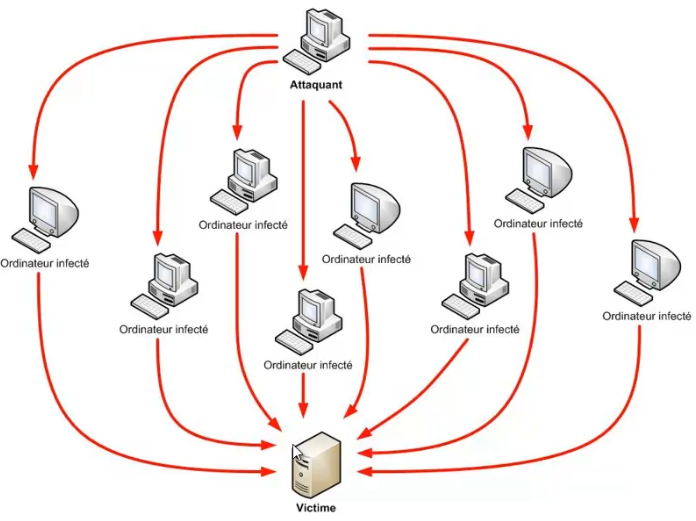
\includegraphics[height=10cm]{IMAGES/ORIGINALS/Architecture_attaque_DDoS}
		\end{center}
		\caption{Architecture d'attaque DDoS}
	\end{figure}
	\section{Principe de fonctionnement des attaques DDoS}
	Une attaque DDoS implique pour un attaquant de prendre le contrôle d'un réseau de machines en ligne afin de mener une attaque. Les ordinateurs et autres machines (comme les objets connectés) sont infectés par un malware, qui les transforme en bots (ou zombies). Le pirate contrôle alors à distance le groupe de bots, appelé un botnet.\\
	
	Un Botnet est une contraction des termes « robot » et « network » où chaque appareil infecté est appelé bot. Il fait référence à un groupe d'ordinateurs qui ont été infectés par des logiciels malveillants et qui sont tombés sous le contrôle d'un attaquant. Les botnets peuvent être conçus pour accomplir des tâches illégales ou malveillantes, notamment l'envoi de spam, le vol de données, les ransomwares, les clics frauduleux sur les publicités ou les attaques par déni de service distribué (DDoS).\\
	
	Une fois qu'un botnet a été mis en place, l'attaquant est en mesure de diriger les machines en envoyant des instructions de mises à jour à chaque bot via une méthode de contrôle à distance. Quand l’adresse IP d'une victime est ciblée par le botnet, chaque bot répond en envoyant des requêtes à la cible, ce qui peut saturer le serveur ou le réseau ciblé, entraînant un DoS pour le trafic normal. Étant donné que chaque bot est un périphérique Internet légitime, il peut être difficile de séparer le trafic d'attaque du trafic normal \cite{cloudflareddos}.
	\section{Catégories d’attaque DDoS}	
	Le nombre d’attaques par déni de service distribué s’est considérablement élevé au cours des dernières années. Ces attaques sont aujourd’hui fréquentes, et peuvent viser toute entité disposant d’un système d’information ou d’une infrastructure réseau connectée à Internet.\\
	
	Les botnets ciblent des vulnérabilités dans différentes couches d’interconnexion des systèmes ouverts et un vecteur d’attaque peut généralement être classé dans l’une des trois grandes catégories suivantes \cite{netscoutddos} : attaques par déni de service volumétriques, attaques par déni de service d’épuisement d’états TCP (TCP state-exhaustion attacks), et attaque de la couche d’application.
	\subsection{Attaques de la couche d’application}
	Généralement appelées attaques DDoS de couche 7 (en référence à la $7^{ième}$ couche du modèle OSI), le but est d'épuiser les ressources de la cible. Les attaques ciblent la couche où les pages Web sont générées sur le serveur et livrées en réponse aux requêtes HTTP. Une seule requête HTTP est peu coûteuse à exécuter côté client et peut coûter cher au serveur cible de répondre car le serveur doit souvent charger plusieurs fichiers et exécuter des requêtes de base de données afin de créer une page Web. Ces attaques sont souvent difficiles à empêcher car le trafic peut être difficile à détecter comme malveillant.\\
	La prolifération des dispositifs IoT non sécurisés au cours des dernières années a été avantageux pour les attaquants DDoS car il existe désormais un nombre presque illimité de dispositifs intelligents qui peuvent être utilisés comme botnet pour lancer des attaques de couche application plus avancées.

	\subsubsection{HTTP Flood}
	\begin{figure}[h]
		\begin{center}
			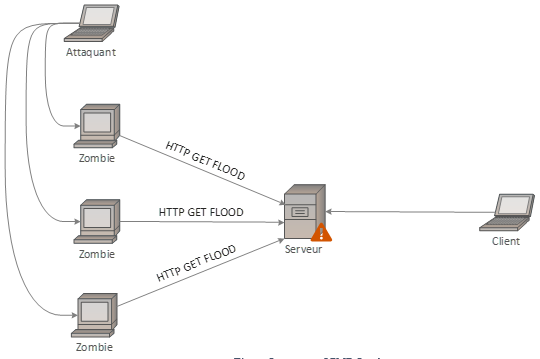
\includegraphics[height=7cm]{IMAGES/ORIGINALS/Attaque_HTTP_Flood}
		\end{center}
		\caption{Attaque HTTP Flood}
	\end{figure}

	Dans une attaque DDoS HTTP Flood, l'attaquant exploite des requêtes HTTP POST ou GET généralement légitimes pour attaquer une application ou un serveur Web. Les HTTP Flood n'utilisent pas de paquets malformés, de techniques de réflexion, ou d'usurpation et nécessitent moins de bande passante que les autres attaques pour faire tomber le serveur ou le site ciblé. L'attaque est plus efficace lorsqu'elle oblige le serveur ou l'application à allouer le maximum de ressources possible en réponse à chaque requête.
	\subsubsection{Slowloris}
	C’est un outil d’attaque écrit en Perl, créé par RSnake (Robert Hansen), une attaque de type DoS hautement ciblée, permettant à une machine de faire tomber un serveur en épuisant les ressources de connexion notamment des serveurs web sans affecter les autres services ou ports du réseau cible. Il y parvient en maintenant ouverts autant de connexions au serveur Web cible que possible. Il accomplit cela en créant des connexions au serveur cible, mais en n'envoyant qu'une demande partielle. Slowloris envoie constamment plus d'en-têtes HTTP, mais ne termine jamais une demande. Le serveur ciblé garde ouverte chacune de ces fausses connexions. Cela déborde finalement le pool de connexions simultanées maximum et conduit au refus de connexions supplémentaires de clients légitimes.\\
	
	Lorsque de nombreux hôtes malveillants lancent simultanément des attaques Slowloris depuis un botnet, toutes les connexions disponibles vers un serveur cible sont ouvertes en même temps. Par conséquent, le serveur ne peut pas gérer les requêtes HTTP légitimes.

	\subsubsection{Imitation de la navigation des utilisateurs}
	Les botnets sont devenus de nos jours les principaux moteurs des activités malveillantes dans le cyberespace. Pour soutenir leurs réseaux de botnet et masquer leurs actions malveillantes, les détenteurs de ces réseaux imitent des cyber-comportements légitimes pour passer inaperçus. Le but de ces attaques est de submerger le site Web ciblé avec un volume suffisamment élevé de botnets, rendant ainsi impossible le trafic légitime ou le plantage du site. Le motif commun derrière de telles attaques DDoS peut être financier ou politique.\\

	Une méthode courante utilisée pour empêcher ce type d'attaque consiste à utiliser une sorte de contrôles captcha, affichant des images ou des modèles auxquels un humain est capable de répondre, mais un bot aurait du mal à le faire
	\subsection{Attaques d'épuisement d'état TCP}
	Les attaques protocolaires, également appelées attaques d'épuisement d'état (state-exhaustion attack), provoquent une interruption de service en consommant toute la capacité des tables d'état disponible des serveurs d'applications Web ou des ressources intermédiaires comme les pare-feu et les répartiteurs de charge. Les attaques protocolaires utilisent les faiblesses des couches 3 et 4 de la pile protocolaire du modèle OSI pour rendre leur cible inaccessible. Ces attaques sont généralement utilisées par des attaquants déterminés qui surveillent et ajustent leurs attaques pour un maximal d'impact .\\
	
	Les attaques courantes d'épuisement d'état peuvent inclure: SYN Flood, SSL/TLS Exhaustion, DNS Flood, attaque Smurf (dans le cadre du protocole ICMP).

	\subsubsection{SYN Flood}
	\begin{figure}[H]
		\begin{center}
			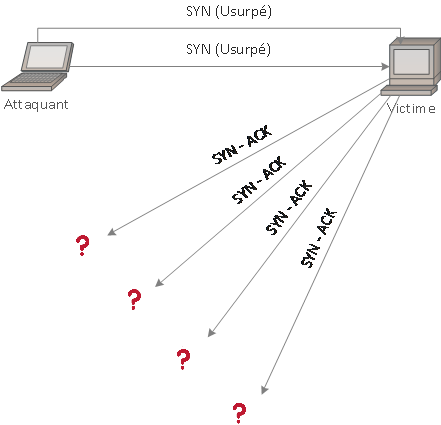
\includegraphics[height=7cm]{IMAGES/ORIGINALS/Attaque_SYN_Flood}
		\end{center}
		\caption{Attaque SYN Flood}
	\end{figure}
	
	Une attaque DDoS SYN flood exploite une faiblesse connue de la séquence de connexion TCP (the « Three-Way Handshake »), dans laquelle une demande SYN pour établir une connexion TCP avec un hôte doit être répondue par une réponse SYN-ACK de cet hôte, et puis confirmé par une réponse ACK du demandeur. Dans un scénario SYN Flood, le demandeur envoie plusieurs demandes SYN à partir d'une adresse IP usurpée, qui ne peut pas répondre à la requête SYN-ACK de l'hôte. Le système hôte continue d'attendre l'accusé de réception pour chacune des demandes, liant les ressources jusqu'à ce qu'aucune nouvelle connexion ne puisse être établie, et entraînant finalement un déni de service.

	\subsubsection{Attaque Smurf}
	\begin{figure}[H]
		\begin{center}
			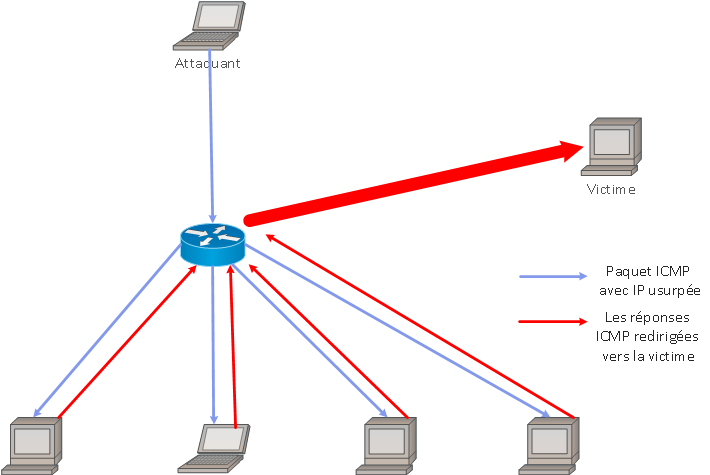
\includegraphics[width=\textwidth]{IMAGES/ORIGINALS/Attaque_Smurf}
		\end{center}
		\caption{Attaque Smurf}
	\end{figure}
		
	Le nom Smurf vient du code source de l'outil d'exploitation original, smurf.c, créé par un individu appelé TFreak en 1997 \cite{ciscoguideagainstddos}. 
Les attaques de Smurf sont quelque peu similaires aux ICMP Flood, car les deux sont effectuées en envoyant une flopée de paquets de demande d'écho ICMP.
Contrairement à ICMP Flood régulière, Smurf est un vecteur d'attaque d'amplification qui augmente son potentiel de dégâts en exploitant les caractéristiques des réseaux de diffusion.\\
	Dans une attaque smurf, un attaquant diffuse un grand nombre de paquets ICMP avec l'adresse IP source usurpée de la victime vers un réseau utilisant une adresse de diffusion IP. Cela oblige les périphériques du réseau à répondre en envoyant une réponse à l'adresse IP source.
	\subsubsection{DNS Flood}
	\begin{figure}[H]
		\begin{center}
			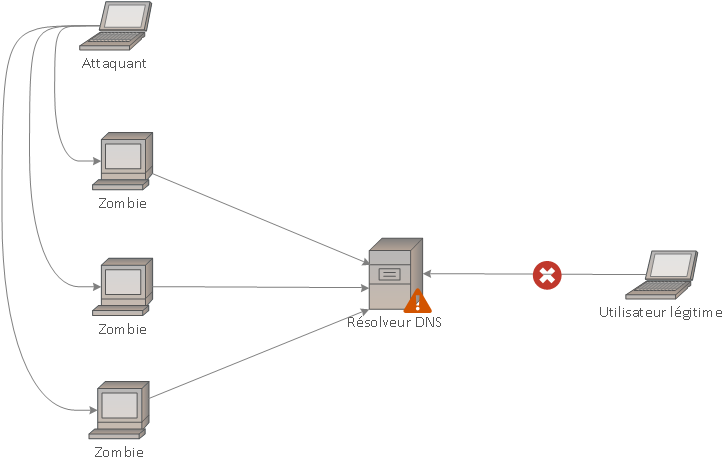
\includegraphics[height=7cm]{IMAGES/ORIGINALS/Attaque_DNS_Flood}
		\end{center}
		\caption{Attaque DNS Flood}
	\end{figure}
	Un DNS Flood est un type d'attaque DDoS où un attaquant submerge les serveurs DNS d'un domaine particulier dans le but de perturber la résolution DNS de ce domaine. Si un utilisateur n'est pas en mesure de trouver le répertoire, il ne peut pas rechercher l'adresse afin d'effectuer l'appel pour une ressource particulière. En perturbant la résolution DNS, une attaque par inondation DNS compromettra la capacité d'un site Web, d'une API ou d'une application Web à répondre au trafic légitime.\\

	Les attaques par inondation DNS utilisent les connexions à large bande passante des caméras IP, d'autres appareils IoT pour submerger directement les serveurs DNS des principaux fournisseurs. Le volume de demandes des appareils IoT submerge les services du fournisseur DNS et empêche les utilisateurs légitimes d'accéder aux serveurs DNS du fournisseur.\\

	Ces attaques DNS diffèrent des attaques par amplification DNS. Contrairement aux inondations DNS, les attaques d'amplification DNS reflètent et amplifient le trafic des serveurs DNS non sécurisés afin de masquer l'origine de l'attaque et d'augmenter son efficacité.	
	\subsection{Attaques volumétriques}
	L’inaccessibilité d’une machine peut être réalisé en surchargeant la bande passante avec des volumes significativement élevés de trafic malveillant. Les attaques DoS et DDoS ciblent directement les réseaux ainsi que leurs périphériques de connexion. Un routeur ne peut traiter qu’une certaine quantité de données à la fois, si cette capacité est dépassée en raison notamment d’une attaque, les services correspondants ne seront alors plus fonctionnels pour les autres utilisateurs.
Les attaques volumétriques sont généralement lancées contre une cible spécifique, généralement des services critiques de fournisseur de services (SP) ou des clients d'entreprise. Les modèles d’attaque sont principalement : ICMP Flood, UDP Flood, IPSec Flood, IP/ICMP Fragmentation, attaques d’amplification de réflexion. 

	\subsubsection{UDP Flood}
	Une UDP Flood est une forme d'attaque volumétrique par déni de service (DoS). Par définition, c’est toute attaque DDoS qui attaque une cible avec des paquets UDP (ne nécessitant pas d’établissement de connexion préalable ou de session). Le but de l'attaque est d'inonder des ports aléatoires sur un hôte distant. Cela oblige l'hôte à vérifier à plusieurs reprises l'application qui écoute sur ce port et (lorsqu'aucune application n'est trouvée) répond avec un paquet ICMP « Destination inaccessible »\cite{impervaddos}. Ce qui conduit à l’inaccessibilité.\\
	Lorsque des attaques par UPD Flood émanent de plusieurs machines, l'attaque est considérée comme une menace de déni de service distribué (DDoS).

	\subsubsection{ICMP Flood}	
	\begin{figure}[H]
		\begin{center}
			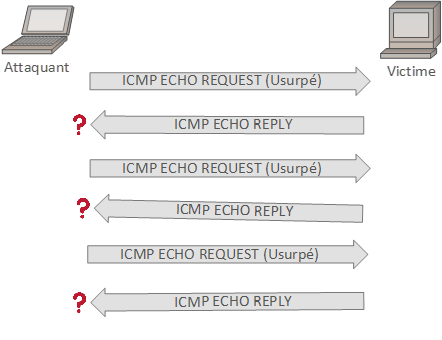
\includegraphics[height=7cm]{IMAGES/ORIGINALS/Attaque_ICMP_Flood}
		\end{center}
		\caption{Attaque ICMP Flood}
	\end{figure}
		
	Similaire en principe à l'attaque UDP Flood, une ICMP Flood submerge la ressource cible avec des paquets de requête d'écho ICMP (ping), envoyant généralement des paquets le plus rapidement possible sans attendre de réponses. Généralement, les messages de demande d'écho et de réponse d'écho ICMP sont utilisés pour envoyer une requête ping à un périphérique réseau afin de diagnostiquer l'intégrité et la connectivité du périphérique et la connexion entre l'expéditeur et le périphérique.\\
	
	Ce type d'attaque peut consommer de la bande passante sortante et entrante, car les serveurs de la victime tentent souvent de répondre avec des paquets de réponse d'écho ICMP, ce qui entraîne un ralentissement global significatif du système. Cette attaque peut être réalisé à l’aide d’outils personnalisé ou code tels que hping and scapy. Elle nécessite au préalable la connaissance de l’adresse IP de la cible.

	\subsubsection{Fragmentation IP/ICMP}
	Une attaque par fragmentation IP/ICMP (soit Internet Protocol / Internet Control Message Protocol) est une forme courante d'attaque volumétrique par déni de service (DoS). Dans une telle attaque, les mécanismes de fragmentation des datagrammes sont utilisés pour submerger le réseau.\\
	Le processus de fragmentation IP est un processus de communication dans laquelle les datagrammes IP sont décomposés en petits paquets, transmis sur un réseau puis réassemblés dans le datagramme d'origine.\\
	La fragmentation est indispensable pour la transmission des données, puisque chaque réseau a une limite unique en matière de taille de datagrammes qu'il peut traiter, qu’on appelle unité de transmission maximale (Maximum Transmission Unit soit MTU). Si le datagramme envoyé est plus grand que le MTU du serveur de réception, il doit être fragmenté pour être transmis complètement.\\

	Dans le cas d’une attaque DoS, l'attaquant peut utiliser la fragmentation IP pour cibler les systèmes de communication, ainsi que les composants de sécurité. Les attaques de fragmentation basées sur ICMP soumettent généralement de faux fragments qui ne peuvent pas être défragmentés. Cela entraîne à son tour le placement des fragments dans un stockage temporaire, occupant de la mémoire et dans certains cas épuisant toutes les ressources de mémoire disponibles.
	\subsubsection{Amplification DNS}
	\begin{figure}[H]
		\begin{center}
			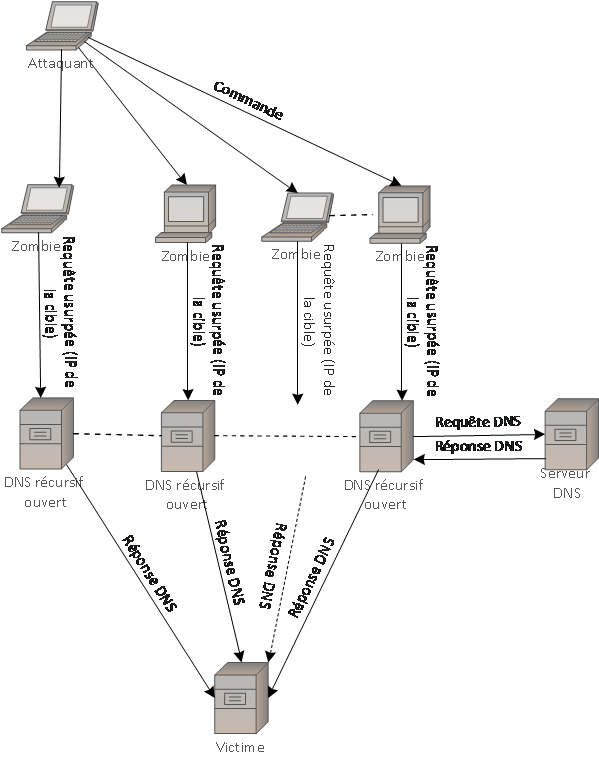
\includegraphics[width=\textwidth,height=15cm]{IMAGES/ORIGINALS/Amplification_DNS}
		\end{center}
		\caption{Architecture d'attaque par amplification DNS}
	\end{figure}	
			
	Les attaques par amplification DNS renforcent la force des attaques de DDoS. Plutôt que d’envoyer le trafic directement d’un botnet à une victime, le botnet envoi des demandes à d’autres systèmes. Ces systèmes répondent en envoyant des volumes de trafic plus importants à la victime. La figure 7 est une illustration de ce type d’attaque.	
	\subsection{Attaques Zero-day}
La définition « Zero-day » englobe toutes les attaques inconnues ou nouvelles, exploitant des vulnérabilités pour lesquelles aucun correctif n'a encore été publié.
En général, le terme attaque Zero-Day (ou attaque 0-day) est utilisé pour les attaques qui utilisent de nouvelles vulnérabilités de sécurité logicielle, dont la communauté n'est pas encore au courant. Cela peut prendre un certain temps entre le moment où le malfaiteur détecte la vulnérabilité et la publication et l'installation du nouveau patch (correctif). Pendant tout ce temps, la vulnérabilité sera activement utilisée pour bloquer les ressources et voler des informations.\\ 

	Par exemple, pour organiser une attaque DDoS réussie, le pirate informatique doit mettre en place un réseau de zombie en peu de temps. La tactique de vulnérabilité Zero-Day est un choix parfait à cet effet. Par conséquent, cette approche gagne en popularité auprès des pirates du monde entier. Pour atteindre leur objectif, les malfaiteurs doivent accéder à un serveur qui exécute un logiciel avec une vulnérabilité de Zero-day. Le serveur peut alors être utilisé pour ce type d'attaques. Cela signifie également qu'il n'est pas nécessaire d'utiliser un grand nombre de machines compromises.\\
	Le terme zero-day est bien connu des membres de la communauté des pirates informatiques, où la pratique du trading de vulnérabilités zero-day est devenue une activité populaire.
	\section{Motivations}
	L'attaques DDoS devient rapidement le type de cyber-menace le plus répandu. Étant donnée la facilité de mises en place des attaques DDoS à faible coût avec très peu de préparation, il est devenu clair que toute organisation court le risque de subir une attaque à tout moment. Mais qu’est-ce qui peut motiver l’auteur d’une attaque ? 
Voici quelques-unes des raisons\cite{bellitddos}.
\subsection{Cyberactivisme}
	Le Cyberactivisme, soit en anglais (Hacktivism). Le DDoS peut servir souvent un mode de protestation contre les sociétés et les gouvernements dont les actions sont considérées comme « incorrectes » ou « mauvaises » par l’attaquant. Par exemple des attaques par des groupes comme Anonymous contre des organisations telles que l’État islamique et le FBI) au personnel et au mesquin (comme des serveurs de jeux informatiques en ligne mis en panne par des joueurs irrités au sujet de changements récents apportés au jeu).
	\subsection{Vandalisme}
	Parfois des attaquants mettent un site Web en panne simplement pour prouver qu’il est possible de le faire, ou pour nulle autre raison que de « se faire remarquer » par une communauté d’utilisateurs en ligne. On attribue ces types d’attaques à ce qu’il est convenu d’appeler des « pirates adolescents » (script kiddies en anglais), en raison de la puérilité des motifs.
	\subsection{Concurrence}
	Si le site Web d’une entreprise donnée tombe en panne, c’est une bonne nouvelle pour ses concurrents. L’entreprise touchée perdra non seulement des ventes, mais sa réputation en prendra également un coup et ses clients pourront affluer vers la concurrence à la place.
	\subsection{Extorsion}
	Les attaquants utilisent des attaques DDoS ou la menace d'attaques DDoS comme moyen d'extorquer de l'argent à leurs cibles. De telles attaques se déroulent souvent de la manière suivante: les attaquants perturbent un site pendant une courte période avec une attaque par déni de service distribué, envoient une note de rançon menaçant de perturber davantage, et si la rançon n'est pas payée, il arrive parfois de faire face à cette menace
	\subsection{Diversion}
	Le DDoS peut également servir de « rideau de fumée » pour dissimuler la véritable cible d’une cyberattaque. Pendant que les équipes de TI s’activent à régler une panne de site Web ou de serveur qui les a détournées de leur attention sur leur vrai travail, il devient plus facile de s’infiltrer furtivement dans le réseau interne de l’entreprise pour lui voler des données financières ou sur ses clients.
\section{Prévention contre les attaques DDoS}
	Les attaques par déni de service distribué (DDoS) représentent une menace importante pour la continuité de l’activité d’un système d’information. Les entreprises, les entités gouvernementales et les particuliers sont devenus de plus en plus dépendantes d’internet, des services web et des applications. La disponibilité de ces systèmes est devenue aussi essentielle que l’électricité.\\

	Les attaques DDoS sont relativement difficile à arrêter, une fois que les machines compromises ont commencé à attaquer la cible. Les conséquences d’une attaque DDoS peuvent être multiples. En effet, la perte de disponibilité d’un service ou d’une application peut provoquer la colère des clients, une perte financière (de revenus) et porté atteinte à l’image de l’entreprise. Lorsque les applications critiques deviennent indisponibles, les opérations et la productivité sont paralysées.\\

	Compte tenu de la nature très médiatisée des attaques par déni de service distribué et de leurs conséquences potentiellement dévastatrices, plusieurs mesures de sécurité ont étés mises au point afin de contrer les surcharges des systèmes de celles-ci.   
Une des solutions peut être d’identifier des adresses IP critiques et de combler les failles de sécurité, par exemple. Ces contre-mesures sont tels que : Ip-Blacklist, filtrage, load balancer, etc.
Des services permettent de contrôler les connexions en amont. Par exemple, Cloudflare qui va mettre l’utilisateur sur une page d’attente pour légitimer ou non sa connexion. Solution viable pour les professionnels.\\

	La principale difficulté pour empêcher une attaque DDoS est de différencier le trafic d'attaque du trafic normal. Par exemple, si un site Web est surchargé de demandes de clients pressés de découvrir la nouvelle version d'un service, ce serait une erreur d'interrompre tout le trafic. En revanche, si cette société connaît brusquement une hausse du trafic provoquée par des acteurs malveillants connus, il est judicieux de prendre des mesures pour limiter l'attaque. Toute la difficulté réside dans le fait qu'il faut distinguer le trafic lié aux clients légitimes de celui provenant de l'attaquant.
	\subsection{Rate limiting}
	La limitation du nombre de demandes qu'un serveur acceptera sur une certaine période est un moyen de réduire les attaques par déni de service. Le rate limiting est utilisé généralement pour contrôler le débit du trafic envoyé ou reçu sur une interface réseau. Toutefois, bien que la limitation du débit soit utile pour ralentir les extracteurs de données Web et atténuer les tentatives de connexion par force brute, seule, elle risque fort d'être insuffisante pour gérer une attaque DDoS complexe efficacement. La limitation du débit reste néanmoins un élément utile dans une stratégie efficace de réduction des attaques DDoS.

	\subsection{Routage de trou noir (blackhole routing)}
	Le routage / filtrage de trou noir DDoS (parfois appelé blackholing) est une contre-mesure pour atténuer une attaque DDoS dans laquelle le trafic réseau est acheminé vers un « trou noir » et est perdu. Lorsque le filtrage du trou noir est mis en place sans critères de restriction spécifiques, le trafic réseau légitime et malveillant est acheminé vers une route nulle ou un trou noir et supprimé du réseau. Lorsque vous utilisez des protocoles sans connexion tels que UDP, aucune notification des données perdues ne sera renvoyée à la source. Avec les protocoles orientés connexion comme TCP, qui nécessitent une prise de contact pour se connecter au système cible, une notification sera renvoyée si les données sont abandonnées. Si un site Internet subit une attaque DDoS, le fournisseur d’accès à Internet (FAI) peut envoyer le trafic entier du site vers un trou noir comme défense.
\subsection{Pare-feu d’application web}
	Un pare-feu d’application web en anglais (Web Application Firewall soit WAF) est un logiciel de traitement de paquets d’état conçu pour arrêter les attaques d’applications basées sur le Web et n’arrête donc pas tous les types d’attaque DDoS tels que les attaques d’épuisement d’état TCP. Toute attaque de réflexion ou d’amplification d’une attaque d’inondation à l’aide de nombreuses sources bot submergerait le WAF et rendrait l’ensemble de la solution inutile. En bref, ces deux technologies sont complémentaires dans leur utilisation pour protéger les organisations contre les attaques, mais un WAF ne protègera pas les vecteurs des attaques DDoS complexes.
Il peut aider à atténuer une attaque DDoS de la couche 7 du modèle OSI. Un atout majeur d’un WAF est sa capacité à mettre en place rapidement des règles personnalisées en réponse à une attaque.
	\section{Conclusion} 
	Les attaques par déni de service distribué (DDoS) se produisent généralement à l’aide d’un botnet. L’attaquant utilise un réseau d’ordinateurs infectés par des logiciels malveillants pour une flopée de trafic vers une cible, comme un serveur. Le but est de surcharger la cible et de ralentir ou de l’écraser.\\
	Les vecteurs d’attaque DDoS sont généralement classés en trois grandes catégories tels que : attaques volumétriques, attaques d’épuisement d’états TCP (TCP state-exhaustion attacks), et attaque de la couche d’application.\\
	L’accès aux services d’une entité doit être restreint afin de n’autoriser que les réseaux internes à celle-ci. Par ailleurs, la mise en place de règles de rate-limiting (limiter le nombre de demandes qu'un serveur acceptera sur une certaine période) peut réduire une éventuelle participation à une attaque par DDoS. Le WAF aussi permet de diminuer les attaques DDoS. Mais la plupart de ces protections classiques sont généralement inefficace face aux attaques DDoS qui sont de plus en plus sophistiquées.\\
	Enfin, le trafic sortant de l’entité doit être filtré afin de bloquer l’envoi de trafic pour lequel les adresses IP sources sont usurpées.


%%%%%%%%CONTRIBUTIONS%%%%%%%%%%
\secondpart
\chapter{Le Deep Learning et les Techniques de Détection d'intrusions}
\minitoc
\thispagestyle{empty}
\newpage	
	
	\section{Introduction}
Comme nous l'avons vu dans les chapitres précédents qu'une fois que les appareils connectés à l'Internet, ils deviennent vulnérables à d'éventuelles attaques informatiques et avec la croissance du nombre d'objets connectés ainsi que les menaces dont fait face l'IoT, il est fortement primordial d'assurer la sécurité des données et des objets connectés.\\  
	La meilleure façon de protéger un réseau ou un système informatique est de détecter les attaques et de se défendre avant même qu’elles ne se produisent. Pour cela beaucoup font appel aux systèmes de détection d’intrusion(IDS) et des systèmes de prévention d'intrusions (IPS) afin de détecter les attaques que peut subir une machine ou le réseau.\\Ces systèmes de surveillance du réseau et des hôtes sont devenus pratiquement indispensables dû à l'incessant accroissement en nombre et en dangerosité des attaques ces dernières années.
	
Par exemple pour assurer l'intégrité des maisons et la sécurité de leurs propriétaires certaines personnes équipent leurs  maisons de systèmes d'alarme qui se déclenchent pour prévenir les propriétaires ou les autorités contre toute effraction ou intrusion dans la maison. \\
De même que le système d'alarme signale l'intrusion dans une maison, le système de détection d'intrusion signale aussi l'intrusion dans une machine ou dans un réseau.\\    

Les systèmes de détection d'intrusion tiennent leur origine de l'armée Américaine qui a initié pour la première fois les techniques de détection d’intrusions en 1980 \cite{refids}. Par la suite plusieurs projets de recherches sur le sujet ont vu le jour dont certains furent couronnés de succès. Avec l'apparition du machine learning et du deep learning de récents travaux utilisant ses techniques d'apprentissages intelligentes ont données des résultats promettants \cite{refidsann} \cite{6664371} \cite{articleids}.\\
  
  Dans ce chapitre, nous présentons premièrement les systèmes de détection d'intrusion, ses diverses caractéristiques, les différents types d'IDS. Ensuite nous exposons le Deep Learning, son origine et ses différents modèles. Enfin on présentera notre approche résiliente pour l'identification et la détection des attaques DDoS dans les réseaux IoT basée sur les modèles de Deep Learning.	
	\section{systémes de détection d'intrusion}
	\subsection{Définition }
Un Système de détection d'intrusion(IDS) est un composant logiciel ou matériel spécialisé, dont le rôle est de surveiller l'activité d'un réseau ou d'un hôte en vue de détecter toute effraction dans l’utilisation des ressources.\\
L’ef{\kern0pt}fraction ou l’intrusion est définie comme une pénétration illégale dans un système, une tentative d’un utilisateur du système d'obtenir des privilèges non autorisés, ou bien toute tentative de viol de la politique de sécurité \cite{zaidi}. Cela veut dire qu'elle peut être d'origine intérieure ou  d'origine extérieure.\\

Vu l'évolution de la complexité des attaques et l'hétérogénéité du trafic des objets connectés ainsi que les dif{\kern0pt}férents paramètres entrant en jeu dans le processus de détection, la détection des intrusions devient une tâche très complexe. Néanmoins, il existe plusieurs travaux de recherches qui ont abouti à de multiples approches et de résultats promet{\kern0pt}tants.
\subsection{Architecture de base d'un IDS}
Plusieurs architectures ont été proposées pour décrire les dif{\kern0pt}férents éléments intervenants dans un système de détection d’intrusion. Il y a trois modules communs à la majorité des architectures IDS proposées\cite{zaidi} : la source de données, l’analyseur des données et le module des réponses.
\begin{itemize}
\item\textbf{la source de donnnées :} ou senseur joue le rôle de collecteur d'informations, telles que les données de trafic sur le réseau ou les données log et les transmet ensuite à l'analyseur. Un IDS peut contenir plusieurs senseurs qui doivent être placée à une position stratégique pour une meilleure qualité de détection du système.
\item\textbf{L'analyseur :} son rôle est d'analyser les données reçues des senseurs et indiquer s'il y a eu anomalie ou pas.
\item\textbf{Le module de réponse :} comme son nom l'indique, il s'occupe de la réponse de l'IDS face aux anomalies détectées. Ça peut être un simple message d’alerte, une sauvegarde dans un fichier log ou bien une interruption de la connexion.   
\end{itemize}
\subsubsection{Architecture CIDF}
Le Common Intrusion Detection Framework (CIDF) est un effort visant à développer des protocoles et des interfaces de programmation d'application afin que les projets de recherches sur la détection d'intrusion puissent partager des informations et des ressources pour que les composants de détection d'intrusion puissent être réutilisés dans d'autres systèmes \cite{refcief}.
L'architecture CIDF, utilise quatre modules : Générateur d'événements, Analyseur d'événements, Unité de réponse et une Base de données d'événements. Les trois premiers modules jouent les mêmes rôles que ceux cités dans la section précédente. Tandis que la Base de données des événements est utilisée pour le stockage des évènements et des données analysées \cite{zaidi}
\cidf
\subsubsection{L’architecture IDWG}
Dans l'architecture proposée par le groupe Intrusion Detection exchange format Working Group (IDWG) de l'IETF, on trouve les trois modules cités précédemment couplés avec d’autres composants. Dans cette architecture, l’objectif était la définition d’un standard de communication entre les composants d'un IDS. Cette architecture définit un format d'échange de message pour les IDS. 
\idwg
Cette architecture est composée des modules suivants\cite{zaidi} :
\begin{itemize}
\item \textbf{source de données :} c’est l’interface entre le système surveillé et l’IDS, elle fait la collecte d’informations sur les activités du système.
\item \textbf{Capteur :}chargé de filtrer et de formater les informations brutes envoyées par la source de données. Le résultat de ce traitement sera un message formaté, appelé aussi événement, il représente l'unité de base dans un scénario d'attaque.
\item \textbf{Analyseur :} permet d’analyser les évènements générés par le capteur. S’il détecte une activité intrusive, il émet une alerte qui est un message sous un format standard. Dans cette architecture, le capteur et l’analyseur forment ensemble une sonde.
\item \textbf{Manager :}en plus de la notification des alertes, il offre à l’administrateur la possibilité de configurer une sonde et de gérer les alertes envoyées par l’analyseur.
\end{itemize} 
\subsection{Classification des systèmes de détection d'intrusion}
Les IDS peuvent être classés selon leur architecture, la provenance de leurs données ainsi que selon leur approche de détection et de réponse\cite{articletypeids}. La figure \ref{ids} résume ses dif{\kern0pt}férents types d'IDS\label{classification}
\typeids
\subsubsection{L’emplacement d’IDS }
%généralement placée derrière le par-feu pour une meilleur
Il existe trois types d'IDS selon l'emplacement de la source de l'information où ils opèrent. Ces sources d'information représentent les paquets capturés à partir des réseaux, des fichiers des systèmes d'exploitation, des logiciels ou encore à partir des fichiers log.
\paragraph{Détection d'intrusion basée sur l'hôte (HIDS) : }
Un système de détection d'intrusion basé sur l'hôte est un IDS spécifique à un hôte unique. il analyse exclusivement l'information concernant cet hôte et surveille son système contre les attaques internes et externes. 
L'IDS est installé sur le système lui-même, une Position idéal pour filtrer avec précision l'ensemble du trafic venant d'extérieur vers cet hôte. 
Les HIDS sont en général placés sur des machines sensibles, susceptibles de subir des attaques et possédantes des données sensibles pour l’entreprise.
\hids
\paragraph{ Détection d'Intrusion basée sur une application (AIDS):} 
Les IDS basés sur les applications (AIDS) sont un sous-groupe des IDS
hôtes. Ils contrôlent l'interaction entre un utilisateur et une application en ajoutant des fichiers log afin de fournir de plus amples informations sur les activités d'une application particulière. Un AIDS se situe
au niveau de la communication entre un utilisateur et l’application surveillée.
L’avantage de cet IDS est sa capacité de détecter et d’empêcher des
commandes particulières dont l'utilisateur pourrait se servir avec le programme et
de surveiller chaque transaction entre l’utilisateur et l’application. De plus, les données sont décodées dans un contexte connu, leur analyse est donc plus fine et précise. Par contre, du fait que cet IDS n’agit pas au niveau du noyau, la sécurité assurée est plus faible, notamment l'attaques de type "Cheval de Troie". Ce type d’IDS est utile pour surveiller l’activité d’une application sensible, mais son utilisation s'effectue en général en association avec un HIDS. Il faudra dans ce cas contrôler le taux d’utilisation CPU des IDS afin de ne pas compromettre les performances de la machine.\cite{reftypeids}
\paragraph{ La Détection d'Intrusion Réseau (NIDS) :}
Un IDS basé sur le réseau est un IDS qui examine le trafic réseau en analysant les paquets par rapport à une base de données contenant des signatures d'attaques connues afin de détecter les anomalies. Il est défini juste à l'entrée du réseau ou entre le réseau et le serveur. L'avantage de cela est que ça permet d'analyser efficacement et rigoureusement le trafic venant de l'extérieur vers le réseau.\\ 
L'implantation d’un NIDS sur un réseau se fait de la façon suivante : des
capteurs sont placés aux endroits stratégiques du réseau et génèrent des alertes s’ils détectent une attaque. Ces alertes sont envoyées à une console sécurisée, qui les analyse et les traites éventuellement. Cette console est généralement située sur un réseau isolé, qui relie uniquement les capteurs et la console. Dans le cadre de réseaux IoT, l'IDS peut être placé au niveau de l'IoT gateway.
\nids
\subsubsection{Mode de détection }
Les systèmes de détection d'intrusion ont été conçu de telle sorte qu'ils puissent détecter et identifier efficacement les menaces.
Deux modes de détection ont été proposées : l'approche comportementale et la
reconnaissance de signatures.
\paragraph{L'Approche comportementale :}\label{comportement}
 La détection d'intrusion par l'approche comportementale consiste à détecter le comportement d'un trafic d'intrus(attaque) par rapport à un profil de trafic habituel(normal) en ce qui concerne la bande passante et le protocole. 
 \begin{comment}
 Sa mise en œuvre comprend : 
\begin{itemize}
\item envoie le jeu de donnée normale(le trafic normal)
\item  phase d'apprentissage au cours de laquelle les IDS apprennent le fonctionnement "normal" des entités surveillés.
\item phase de comparaison de tout le trafic réseau à ce comportement normal appris.
\item déclencher une alerte en cas d'une incohérence avec le comportement normal connu
À titre d’exemple, un projet très ambitieux a été sponsorisé par la DARPA (en 98 et 99), en collaboration avec le laboratoire Lincoln du MIT \cite{refdarpa}. L'objectif était de fournir un jeu de données d'apprentissage comprenant trafic de fond et activités intrusives (c’est-à-dire du trafic intrusif ou des événements systèmes causés par des attaques). Le trafic de fond était déduit des données statistiques collectées sur le réseau des bases de l’Air Force alors que les attaques étaient générées par des scripts créés spécialement, mais aussi par des scripts collectés à travers des sites spécialisés et des listes de diffusion. Les données collectées concernaient à la fois des HIDS et des NIDS.\\ 
\end{itemize}
\end{comment} 
Dans le cas du HIDS, ce type de détection peut être basé sur des informations telles que le taux d’utilisation CPU, l’activité sur le disque, les horaires de connexion ou d’utilisation de certains fichiers (horaires de bureau…).\\
\textbf{Avantages : } les IDS basés sur l'approche comportementale ont des capacités de détecter tous les types d'attaques y compris les Zéro day attaques.
Cette approche permet de produire l'information utile pour la définition des
signatures des IDS à base de signatures\cite{reftypeids}.\\
\textbf{Inconvénients :} Le grand défaut de cette approche est le grand nombre de fausses alertes dues aux comportements imprévisibles des utilisateurs du réseau. Elle exige souvent l’historique à long terme des évènements enregistrés afin de caractériser les modèles normaux de comportement \cite{reftypeids}.
\paragraph{La reconnaissance de signature :}
La détection d'intrusion basée sur la reconnaissance de signatures consiste à la détection d'attaques en recherchant des signatures spécifiques, tels que des séquences d'octets dans le trafic réseau ou des séquences d'instructions malveillantes connues utilisées par des logiciels malveillants. Une signature permet de définir les caractéristiques d’une attaque, au niveau des differentes couches protocolaires du modèle (TCP/IP). Ces signatures proviennent en général des antivirus qui donnent une signature spécifique à chaque types d'attaques. \\
C'est une approche qui utilise les connaissances accumulées sur les attaques spécifiques et les vulnérabilités du système
\begin{comment}
 Sa mise en œuvre comprend : 
\begin{itemize}
\item un jeu de donnée contenant les signatures des attaques connues
\item  phase d'apprentissage au cours de laquelle les IDS apprennent les signatures des attaques.
\item phase de comparaison des données des entités surveillés par rapport aux signatures des attaques connues.
\item déclencher une alerte en cas de similarité entre des données et la base de signature.
\end{itemize}
\end{comment}
\textbf{Avantages : } le plus grand avantage des systèmes de détection d'intrusion basés sur la reconnaissance de signature est qu'il détectent de façon très efficace les attaques dont ils disposent de leur signature sans produire un grand nombre de fausses alertes. \\ 
\textbf{Les inconvénients :}
Les IDS basés sur la reconnaissance de signature ne peuvent pas détecter les attaques dont ils ne possèdent pas les signatures. De ce fait, il nécessite des mises à jour fréquentes de sa base de signature.
Les pirates contournent facilement ces types d'IDS en utilisant les techniques dites "d'évasion" qui consistent à faire varier les signatures des attaques de tels sorte que les IDS ne les reconnaissent plus.
\subsubsection{Types de réponse}
les IDS étant des systèmes très réactifs donc chaque fois qu'une intrusion est détectée, le système déclenche une alerte. cette section décrit comment le système réagira à l'alerte déclenchée. Il existe deux types de réponses : réponse passive et réponse active.
La majorité des IDS existants fournissent une réponse passive. Par contre la réponse active est plus ou moins implémentée\cite{articlepa}.
\paragraph{ La réponse passive :}
La réponse passive d’un IDS consiste à enregistrer les intrusions détectées dans un fichier log qui sera analysé par l'administrateur du système. Cette réaction peut être aussi par l'envoie d'un email ou l'ouverture d'une fenêtre console contenant les détails de l'intrusion. Il est à noter que ce type d'IDS n’empêche pas directement une attaque de se produire, c'est à la charge de l'administrateur système de prendre la décision d'appliquer la politique de sécurité nécessaire pour empêcher l'intrusion de se produire. 
\paragraph{ La réponse active :} 
En plus d'être un IDS passif, Un IDS actif peut stopper une attaque au moment de sa détection. Pour cela, à la détection d'une attaque l'IDS prend des décisions pour modifier l'environnement du système attaqué sans l'intervention requise d'une personne. Cette altération peut consister à la déconnexion de l'attaquant ou la ré-configuration des mécanismes réseaux pour bloquer toutes les connections provenant de la même adresse source.
\subsubsection{La fréquence d'utilisation }
Le mode d'utilisation d'un IDS peut être choisi selon les besoins en fonction du mode d'utilisation : continue (online) ou périodique (offline). 
\paragraph{Utilisation continue :}
L'utilisation continue est une analyse en temps réel(online) c'est-à-dire la détection d'attaques se fait au moment où elle se produit. Le principal avantage est que les alertes sont lancées dès que les attaques sont détectées. Cet état de veille coute cher en termes de ressources et nécessite des algorithmes plus complexes que ceux d'une analyse différé.\cite{reftmqb} 
\paragraph{ Utilisation périodique :}
L'utilisation périodique est une analyse différé(offline) cela veut dire que L'analyse s'effectue sur des données stockées (non fraîches) dans des fichiers logs. Elle est préférable pour avoir une défense plus fiable du point de vue du temps de calcul. En effet pour un IDS online le temps de calcul de l'IDS doit être supérieur au temps du trafic réseau, ce qui est difficilement atteignable et peut affecter considérablement le trafic réseau.
\subsection{Exemples d'IDS existants }
Le marché des IDS est très vaste. Certains produits sont gratuits et d'autres
payants. Voici quelques exemples d'IDS :\\
\textbf{Snort:}
Snort a été créé par Cisco et est considéré comme le leader de l'industrie du NIDS. Il est gratuit et disponible sur Windows et Linux \cite{snort}.  \\
\textbf{Ossec :}
OSSEC est un HIDS gratuit. Il effectue l'analyse des journaux, la vérification de l'intégrité, la surveillance du registre Windows, la détection des rootkits, les alertes en temps réel et la réponse active. Il fonctionne sur la plupart des systèmes d'exploitation notamment Linux, OpenBSD, FreeBSD, MacOS, Solaris et Windows. \cite{ossec}\\
\textbf{Zeek :} Zeek est le nouveau nom de l'ancien IDS "Bro", c'est un analyseur de trafic réseau passif et open source. Il analyse le trafic réseau à la recherche de signes d'activités suspectes. Il est disponible sur Linux, FreeBSD, macOS \cite{zeek}\\
\textbf{Prelude :} Prelude est un IDS hybride (HIDS et NIDS), appelé aussi un système de gestion des informations de sécurité et des événements. Prelude collecte, normalise, trie et détecte les anomalies liés à la sécurité  des entités surveillées. \cite{prelude} 
\begin{comment}
\subsection{Evaluation des IDS}

\end{comment}
\subsection{Critère de choix d'un IDS}
Comme nous l'avons vu dans la section \ref{classification} qu'il existe plusieurs types d'IDS. Chacun de ces IDS présentent des avantages et des faiblesses, c'est pourquoi, il est indispensable de choisir son IDS selon certains critères bien spécifiques. Les critères de sélection sont détaillés ci-dessous \cite{refsecuriteinfo}
\begin{itemize}
\item\textbf{Réactivité :} Un IDS doit être en mesure de détecter les zero day attaques ou nouveaux types d'attaques. Par exemple, l'IDS par l'approche comportementale \ref{comportement}. 
\item \textbf{Facilité d'utilisation et d'adaptabilité :} Un IDS doit être facile à utiliser et surtout s'adapter au contexte dans lequel il doit opérer. Il est inutile d'avoir un IDS émettant des alertes en moins de 10 secondes si les ressources nécessaires à une réaction ne sont pas disponibles pour agir dans les mêmes contraintes de temps \cite{refsecuriteinfo}.
\item\textbf{Performance :} l'installation d'un IDS ne doit en aucun cas affecter les performance des systèmes surveillés. ni affecter la vitesse du trafic réseau. De plus, il faut toujours avoir la certitude que l'IDS a la capacité de traiter toute l'information à sa disposition. Par exemple un IDS réseau doit être capable de traiter l'ensemble du flux pouvant se présenter à un instant donné sans jamais supprimer de paquets car dans le cas contraire il devient trivial de masquer les attaques en augmentant la quantité d'information.\cite{refsecuriteinfo}
\item\textbf{Fiabilité :} Un IDS est fiable s'il détecte quasiment tous les vraie positifs (alerte que lorsqu'il y a attaque) et moins de faux de positifs.
\end{itemize}
\section{Le Deep Learning}
\begin{comment}Dans cette section on donnera un aperçu sur le deep learning, son origine, ses avancées récentes dans les systèmes de détections d'intrusions.\end{comment}
\subsection{Définition et Historique}
Le Deep Learning(DL) ou apprentissage profond est un sous-domaine particulièrement puissant du Machine Learning(ML)ou apprentissage automatique. Ce dernier étant aussi un sous-domaine de l'intelligence artificielle(IA) qui consiste à doter les systèmes informatiques de capacité d'apprendre sans être explicitement programm.\cite{refclassroom}.
\dl
 Le Deep Learning tient ses origines de l'avancement des algorithmes des réseaux de neurones artificiels \ref{RNA}.
Contrairement aux réseaux de neurones artificiels, les méthodes d'apprentissage profond utilisent plusieurs couches cachés(réseau profond) d'où son nom Deep learning en référence aux nombres de couches cachées leurs permettant de résoudre des problèmes complexes\cite{refbookdl}.\\
Les algorithmes à base de DL sont devenus très populaires ces dernières années notamment avec leur succès dans la résolution de problèmes complexes pourtant 
les fondements de ces méthodes ne sont pas si récents. En effet leurs origines remontent en 1943 lorsque McCulloch et Pitts \cite{refhistoiredl} ont publié une étude présentant le modèle mathématique basé sur le neurone biologique. Cela a été mis en œuvre par la suite dans les années 50 par l'invention du Perceptron par le chercheur Frank Rosenblatt\cite{Rosenblatt58theperceptron} ainsi que les travaux de Yan LeCun en 1989\cite{yanlecun1} sur les réseaux de neurones convolutifs.
Longtemps délaissé entre 1989 et 2000 par la communauté scientifique, c'est grâce à l'avènement des données massives(Big Data) et des puissances de calcul phénoménales des processeurs graphiques(GPU) que les chercheurs Yann Le Cun, Yoshua Bengio et Geoffrey Hinton décident en 2003 \cite{yannlecun} de démarrer un programme de recherche dénommé \textit{conspiration de l'apprentissage profond} pour remettre au goût du jour les réseaux neuronaux. 
Suivront de nombreux développements des réseaux de neurones convolutifs et les réseaux de neurones profonds(deep learning) qui en découlent en 2012 et ouvrent la voie à de nombreux champs d'application comme la vision, le traitement du langage, la reconnaissance de la parole ou à la cybersécurité.
\subsection{Les réseaux de neurones artificiels}\label{RNA}
Les réseaux de neurones artificiels (RNA) sont des algorithmes d'apprentissage automatique inspirés du système nerveux humain. Ils sont constitués d'une interconnexion de neurones artificiels ou formels \ref{atn}. Les réseaux de neurones se distinguent par leur architecture, leur niveau de complexité (le nombre de neurones, présence ou non de boucles), par le type de fonctions d'activation utilisé ainsi que par l'objectif visé : apprentissage supervisé ou non \cite{Kim2018}
\subsubsection{Neurone artificiel :}\label{atn} Un neurone artificiel est une abstraction mathématique très simplifiée d’un neurone du cerveau humain. Un neurone biologique reçoit des signaux électriques par ses dendrites, les transforme dans ses synapses et s’active ou non en fonction des signaux reçus. Si un neurone biologique s’active, cela signifie qu’il transmet le signal électrique reçu à d’autres neurones\cite{bioneurone}.\\
	 Comme pour le neurone biologique le neurone formel reçoit des valeurs en entrée, pondère ces valeurs avec des poids (ou coefficients) et retourne une valeur en sortie en fonction de la somme des valeurs pondérées. L'action d'envoyer une valeur par le neurone s'appelle alors une activation. La figure \ref{atnn} illustre un neurone artificiel.
\neurone
	\begin{equation}\label{eqpondere}
	\text{Somme pondérée }    z = \sum_{i=1}^n (X_i \times W_i) + bias
	\end{equation}
	\begin{equation}
		\textbf{Fonction d'activation }  y = \varphi (z)
	\end{equation}
\subsubsection{Reseaux de neurones Profonds(DNN)}\label{dnn}
Comme son nom l'indique, un réseau de neurones profond(DNN) est un réseau composé de multiples couches successives. Une couche est un ensemble de neurones n’ayant pas de connexion entre eux. un modèle de deep learning est dit profond s'il comporte au moins 2 couches cachées, et plus un modèle est profond, plus il apprend et réalise des taches comme les humains. 
\begin{comment}
La figure \ref{perceptro} presente un DNN composé d'une couche d’entrée(3 neurones)qui lit les entrées, deux couches cachés et une couche de sortie qui fournit la réponse du système. L’algorithme que les perceptrons utilisent la rétropropagation du gradient pour mettre à jour leurs poids ce qui les permet d'avoir moins d’erreur dans leur prédiction\cite{RNNCNN}. Nous avons utilisé dans ce mémoire cette représentation dans la définition de notre modèle de deep learning.
\perceptron 
\end{comment} 
Les éléments essentiels qui constituent un DNN sont :\\
\textbf{- La Couche d'entrée} : représente les données d'entrées du réseaux. Par exemple, pour les données textuelles, il peut s'agir de mots ou des personnes, pour une image, il peut s'agir de valeurs pixels brutes provenant de différents canaux de couleur.\\
\textbf{- Les couches cachées :}
Les couches cachées sont des couches situées entre les couches d'entrée et de sortie. Le nombre de couches cachées rend le réseau profond, c'est pourquoi ils sont appelés réseaux de neurones profonds (DNN) et le processus d'apprentissage dans le DNN est le DL\cite{yakuz}.\\
\textbf{- La couche de sortie :}
La couche de sortie représente les valeurs de sortie du réseau. En général, le nombre de neurones dans la couche de sortie est égale au nombre de classe de sortie.\\
\textbf{Les fonctions d'activations : }
La fonction d'activation définit la manière dont chaque neurone artificiel réagit face aux signaux entrants et sortants d'un neurone. Elle permet le passage ou non d’information si un certain seuil est atteint et s'applique sur la fonction suivante : $x = \sum( entrée * poids ) + biais$
\begin{comment}
\paragraph*{-La fonction Step :}Elle renvoi tout le temps 1 pour un signal positif, et 0 pour un signal négatif.\\
\begin{minipage}{.4\textwidth}
\[
 f(x) = 
  \begin{cases} 
   0 & \text{si } x < 0 \\
   1       & \text{si } x \geq 0
  \end{cases}
\] 
\end{minipage}
\begin{minipage}{.3\textwidth}
\begin{tikzpicture}
\begin{axis}[
    axis lines=middle,
    xmax=6,
    xmin=-6,
    ymin=-0.05,
    ymax=2.05,
    xlabel={$x$},
    ylabel={$y$}]
\addplot [domain=-5.5:0, samples=100, thick, blue] {min(0,1)};
\addplot [domain=-0:5.5, samples=100, thick, blue] {max(0,1)};
\end{axis}
\end{tikzpicture}
\end{minipage}
\end{comment}
\paragraph*{- La fonction Sigmoïde :} est utilisé en couche de sortie pour la classification binaire. Ses valeurs sont comprises entre 0 et 1. Son souci est sa perte d'information dans la phase de feed forward et de backpropagation\cite{sigm}.\\
\begin{minipage}{.4\textwidth}
\begin{equation}
	\text{sigmoïde}(x)=\frac{1}{1+e^{-x}}
\end{equation} 
\end{minipage}
\begin{minipage}{.3\textwidth}
\begin{tikzpicture}
\begin{axis}[
    axis lines=middle,
    xmax=10,
    xmin=-10,
    ymin=-0.05,
    ymax=1.05,
    xlabel={$x$},
    ylabel={$y$}
]
\addplot [domain=-8.5:8.5, samples=100, thick, blue] {1/(1+exp(-x))};
\end{axis}
\end{tikzpicture}
\end{minipage}
\paragraph*{- Fonction tangente hyperbolique (tanh) : } 
La différence fondamentale entre les fonctions tanh et sigmoïde est que tanh est centré sur 0. Sa plage de sortie est comprise entre [-1, 1] et est plus efficace que sigmoïde \cite{livredlE}. Cependant elle souffre encore du problème de disparition du gradient \\
\begin{minipage}{.4\textwidth}
\begin{equation}
	\text{tanh}(x)= \frac{e^{x}-e^{-x}}{e^{x}+e^{-x}}
	\label{eqtanh}
\end{equation} 
\end{minipage}
\begin{minipage}{.3\textwidth}
\begin{tikzpicture}
\begin{axis}[
    axis lines=middle,
    xmax=10,
    xmin=-10,
    ymin=-1.05,
    ymax=1.05,
    xlabel={$x$},
    ylabel={$y$}]
\addplot [domain=-9.5:9.5, samples=100,
     thick, blue] {(exp(x) - exp(-x))/(exp(x) + exp(-x))};
\end{axis}
\end{tikzpicture}
\end{minipage}
\paragraph*{- Fonction ReLU : }
Une Unité Linéaire Rectifiée(ReLU) est l'une des fonctions d'activations la plus courante et la plus populaire actuellement à cause de sa rapidité dans l'entrainement des Réseaux de neurones profonds. En effet La fonction ReLU traite le problème du gradient de disparition des précédentes fonctions d'activation (sigmoïde et tanh) ainsi qu'une propagation efficace du gradient dans les réseaux profonds \cite{livredlE}. Elle est très utilisée dans les CNN, RBM, et a un intervalle de sortie $[0, +\infty[$. ReLU souffre du phénomène de ‘Dying ReLU’, auquel on préférera les variantes de ReLU notamment : Leaky ReLU, Parametric ReLU(PReLU), Randomized Leaky (ReLU)etc.\\
\begin{minipage}{.4\textwidth}
\[
 \text{ReLU}(x) = 
  \begin{cases} 
   max(0,x) & \text{si } x \geq 0 \\
   0      & \text{si }  x < 0
  \end{cases}
\] 
\end{minipage}
\begin{minipage}{.3\textwidth}
\begin{tikzpicture}
\begin{axis}[
    axis lines=middle,
    xmax=6,
    xmin=-6,
    ymin=-0.05,
    ymax=5.05,
    xlabel={$x$},
    ylabel={$y$}]
\addplot [domain=-5.5:5.5, samples=100, thick, blue] {max(0, x)};
\end{axis}
\end{tikzpicture}
\end{minipage}
\paragraph*{- La Fonction Softmax :} est utilisée sur la dernière couche pour générer des probabilités décimales à chaque classe(sortie) d'un problème de multi-classification à plusieurs sorties \cite{livredlE} tel que la somme de ces probabilités décimales soit égale à 1. Son intervalle de sortie est $[0, 1]$ : 
\begin{minipage}{.4\textwidth}
\begin{equation}
 \text{Softmax}(x_i) = \frac{e^{x_i}}{\sum_{j=1}^k e^{x_j}}
 \label{eqsoft}
\end{equation} 
\end{minipage}
\begin{comment}
\begin{minipage}{.3\textwidth}
\pgfmathdeclarefunction{sumexp}{3}{%
\begingroup%
\pgfkeys{/pgf/fpu,/pgf/fpu/output format=fixed}%
\pgfmathsetmacro{\myx}{#1}%
\pgfmathtruncatemacro{\myxmin}{#2}%
\pgfmathtruncatemacro{\myxmax}{#3}%
\pgfmathsetmacro{\mysum}{0}%
\pgfplotsforeachungrouped\XX in {\myxmin,...,\myxmax}%
{\pgfmathsetmacro{\mysum}{\mysum+exp(\XX)}}%
\pgfmathparse{\mysum+exp(#1)}%
\pgfmathsmuggle\pgfmathresult\endgroup%
}%
\begin{tikzpicture}
            \begin{axis}[
            axis lines=middle,,
            ylabel=$y$,
            xlabel=$x$,
            xmin=-10,
            xmax=10,
            ymin=-5.05,
    		ymax=5.05]
               \addplot[blue,domain=-5:5,samples=100] 
               {exp(x)/ (\sum_1^5 exp(x))};
            \end{axis}
        \end{tikzpicture}
\end{minipage}
\end{comment}
\subsection{Classification des modèles de Deep Learning}\label{model}
Selon l'architecture et les techniques utilisées par le modèle, Aminanto et  Muhamad Erza \cite{Kim2018} classent les modèles de deep learning en trois catégories : Apprentissage supervisé(génératif), apprentissage non supervisé(discriminatif) et architecture hybride. La figure \ref{typedl} présente une illustration simplifiée de ces différents modèles.
\typedl
\subsubsection{Apprentissage supervisé}
L'apprentissage supervisé est le type d'apprentissage où les modèles apprennent et classent des éléments selon une classe donnée. Une classe représente un groupe d'éléments ayant les mêmes similarités. Les données de la classe cible sont nécessaires pendant la phase d'apprentissage. Le modèle créerait une base de connaissance à partir des informations apprises qu'il utilisera par la suite  pour déterminer la correspondance d'une donnée avec une classe cible. \\
Avec l’apprentissage supervisé, la machine peut apprendre à faire une certaine tâche en étudiant des exemples de cette tâche. Par exemple, elle peut apprendre à reconnaître une photo de chien après qu’on lui ait montré des millions de photos de chiens. Ou bien, elle peut apprendre à traduire le français en chinois après avoir vu des millions d’exemples de traduction français-chinois\cite{refgm}.
\paragraph{Les réseaux de neurones convolutifs : }
inventé par Yann Lecun \cite{yannlecun}, les réseaux convolutifs sont une forme particulière de réseau neuronal multicouches dont l’architecture des connexions est inspirée de celle du cortex visuel des mammifères.
Ils contiennent en général trois types de couches : des couches de convolution, des couches de regroupement(pooling) et des couches entièrement connectées(full connected). Une couche convolutive, est basée comme son nom l’indique sur le principe mathématique de convolution, et cherche à repérer la présence d’un motif (dans un signal ou dans une image par exemple)\cite{convolution}.\\
  La couche convolutive détecte les connexions des entités locales de la couche précédente et la couche de regroupement s'occupe de la tâche de fusionner les entités sémantiquement similaires en une seule entité, enfin la couche entièrement connectée rassemble ces informations pour fournir la sortie(Output). 
 La Figure \ref{cnn} présente une architecture classique d’un réseau de neurones convolutif. Une image est fournie en entrée (input) et est convoluée avec des filtres (première couche de convolution) dont les cartes d’activation sont regroupées et concaténées en sortie. 
 Cette technique est généralement employée pour les techniques de traitement d'image.
%\cnn
 \subsubsection{Apprentissage non supervisé}
Contrairement à  l'apprentissage supervisé, l'apprentissage non supervisé se fait de façon totalement autonome, c'est-à-dire que les données sont envoyées au modèle sans lui fournir des étiquètes attendus comme sortie. Cette technique est utilisée dans la détection d'anomalies, la cybsersécurité, mais aussi dans le dépistage précoce de maladies.\paragraph{ Auto encodeurs : }
L’idée de base derrière les auto-encodeurs est d’encodé des informations et d’apprendre une représentation (encodage) d’un ensemble de données. L’ensemble du réseau ressemble à un sablier, avec des couches cachées plus petites que les couches d’entrées et de sorties. La plus petite couche est toujours au milieu et représente l’endroit où l’information est la plus compressée (le bottleneck). La première moitié est dénommée l'encodage, la seconde moitié le décodage.
%\autoencodeur
\paragraph{Réseaux de neurones récurrents (RNN) :}
Dans un réseau neuronal traditionnel, nous supposons que toutes les entrées (et les sorties) sont indépendantes les unes des autres. Mais pour de nombreuses tâches, cela est une mauvaise conception. Par exemple, si on veut prédire le prochain mot dans une phrase, il faut connaître les mots qui sont venus avant. Les RNN répondent à ce genre de conception en conservant des informations dans leurs unités cachées un «vecteur d'état» qui contiennent implicitement des informations sur l'historique de tous les éléments passés dans la séquence \cite{RNNCNN}. Ils sont appelés récurrents car ils possèdent des connexions récurrentes, c'est-à-dire qu'ils exécutent la même tâche pour chaque élément d’une séquence dont la  sortie est dépendante des calculs précédents. Ils sont beaucoup utilisés dans la prédiction des textes.
Néanmoins, ce transfert d’information à double sens rend leurs entrainements beaucoup plus compliqués, et ce n’est que récemment que des méthodes efficaces ont été mises au point comme les réseaux à large mémoire court-terme(LSTM)\cite{LSTM}. L'utilisation des réseaux LSTM ont révolutionné la reconnaissance de la voix par les machines (Speech Recognition) et la génération automatique de texte
\paragraph{Machines de Boltzmann :}
Les machines de Boltzmann(BM) sont des modèles de Deep Learning génératifs non déterministes capables de prendre des décisions stochastiques\cite{bt}. Un BM est non déterministe du fait qu'il n'a pas de sortie typique comme les autres modèles classiques de deep learning. Elles ont été inventées par Geoffrey Hinton et Terry Sejnowski\cite{histoirebm}. Les BMs sont composées de deux catégories de neurones : les neurones visibles et les neurones  cachés. Dans un réseau BM, tous les neurones sont connectés entre eux qu'ils soient dans la catégorie visible ou dans la catégorie cachée. La Machine Boltzmann restreinte(RBM)\cite{RBM} est un BM personnalisé sans connexions entre les neurones cachés ni entre les neurones visibles(entrées).
\subsubsection{Hybride }
L'architecture profonde hybride combine à la fois des architectures génératives(supervisé) et discriminatives(non supervisé). Un exemple d'architecture hybride est le Réseau Génerateur Adversatif(GAN).
\paragraph{ Génerateurs Adversatifs :} sont constitués de                                                                                                              deux réseaux travaillant en parallèle, l’un ayant pour tâche de générer du contenu (le générateur) et l’autre d’en juger la qualité (le discriminateur). L’objectif des réseaux génératif est d'augmenter le taux d’erreur du réseau discriminant(c’est-à-dire de "tromper" le discriminateur en produisant de nouveaux cas qui semblent provenir de la vraie distribution de la population d’entraînement) \cite{cnn}.
\section{\'Etudes expérimentales}
Cette section présente les différents outils matériels et logiciels utilisés pour la réalisation de notre approche basée sur le deep learning. Premièrement, nous présentons les outils utilisés ensuite l'architecture de notre modèle, une étude du Dataset utilisé ainsi que quelques interfaces graphiques de l'application réalisée. Enfin, on présente nos résultats obtenus ainsi qu'une comparaison avec les autres travaux dans la littérature.   
\subsection{Outils de développement}
les outils matériels et logiciels utilisés pour le développement sont : 
\subsubsection{Materiels}
Notre IDS a été réalisé et testé sur 2 PCs (Personnal Computer)dont les caractéristiques sont les suivants :
\begin{table}[H]
\centering
\begin{tabular}{cccc}
  \toprule
   \textbf{Marque} & \textbf{CPU} & \textbf{RAM} & \textbf{OS} \\
   \midrule
     \textbf{HP Notebook} & AMD Radeon R4 2GHz & 8Go & Windows10 64bits \\
     \textbf{THOSIBA TECRA} & Intel Core i3 2GHz & 8GO & Windows10 64bits \\
  \bottomrule
\end{tabular}
\caption{Caractéristiques du matériels utilisés}
\label{tabmat}
\end{table}
\subsubsection{JAVA} 
Java est un langage de programmation orienté objet crée par Sun Microsystems (aujourd'hui racheté par Oracle) \cite{java}. Plus de 10 millions de développeurs et plus de 15 milliards de périphériques tournent sur java. Connu pour sa portabilité, c’est un langage très populaire car il met à la disposition des développeurs les API, les Framework ainsi que les bibliothèques(library) nécessaires pour la création de programmes riche et robuste. 
Pour la réalisation de notre projet nous avons opté pour la version 1.8 du JDK et le framework JavaFX(pour GUI) qui est devenu depuis la version 8, une référence pour la création des interfaces graphiques.
\subsubsection{DeepLearning4j}
Comme son nom l'indique Deeplearning4J (DL4J) est un framework Java pour le deep learning pour tirer profit de sa portabilité. Il est distribué sous la licence Apache 2.0, open source et écrit en Java et Scala \cite{dl4j}. DL4J a été initié fin 2013 en tant que projet chez Skymind qui rejoint en 2017 la Fondation Eclipse pour sa mise en œuvre. DL4J est actuellement le seul Framework de deep learning qui intègre Hadoop et Spark pour l'entrainement des réseaux de neurones. En effet DL4J utilise Map-Reduce et Spark pour entraîner le réseau tout en s'appuyant sur d'autres bibliothèques notamment les librairies ND4J, DataVec etc. DL4J traite la phase de chargement des données et des algorithmes d'entraînement comme des processus séparés c'est-à-dire distribués le traitement en s'appuyant sur Map-Reduce et spark. Cette séparation du traitement lui offre une grande flexibilité.
DL4J fonctionne sur des CPU et des GPU distribués et possède à la fois une version communautaire et une version entreprise.
\subsubsection{IDE IntelliJ}
IntelliJ est un environnement de développement intégré (IDE) pour le développement de logiciels. Il propose de nombreux outils pour faciliter le développement dont l’auto-complétion syntaxique, une vérification d’erreur en live, différents outils de compilation, des outils de debugging avancés, etc.
\subsection{Mise en œuvre}
Nous avons développé notre approche résiliente avec le langage de programmation JAVA et le framework DL4J. Pour l'entrainement et nos differents tests nous avons utilisé les datasets IoT Botnet et NSL-KDD.
nous présenterons seulement la mise en œuvre en utilisant le dataset IoT Botnet vu que les procédures pré-traitement, entrainement et test sont similaires pour les deux datasets. 
%\newpage
Le développement de notre approche suit l'architecture  suivant :
\architecture
 \subsubsection{Choix du Dataset : }
 \begin{comment}
Pour le choix du jeu de données, nous avons opté pour deux types de jeux de données notamment NSL-KDD et Bot IoT 2020. 
\textbf{NSL-KDD :}\\
Le Dataset NSL-KDD \cite{nslkdd} est une version amélioré du dataset KDD99 \cite{kdd}, proposé en 2010 par les chercheurs dans le domaine de détection d'intrusions dans les réseaux afin de résoudre certains problèmes de redondance apparu dans la base KDD 99. NSL-KDD est considéré comme une référence dans l'évaluation des systèmes détection  d'intrusions. Il présente les améliorations apportés à KDD99 en éliminant les enregistrements redondants dans les données d'apprentissage(Training set) et en supprimant aussi les enregistrements double dans les données de test (Testing set) de KDD99. Il est composé de 41 caractéristiques résumé dans le tableaux ci-dessous : 
\nslkdd
\end{comment}
\textbf{IoT Botnet:}\\
Le dataset Bot-IoT a été développé à l'Université de New South Wales Canberra en Australie \cite{botiot1}. Ce dernier contenait 46 caractéristiques et deux types de trafics réseaux (normal et anormal). Ce dataset reflète des trafics générées depuis un environnement de réseaux IoT.
 En Mars 2020 les chercheurs Imtiaz Ullah et Qusay Mahmoud de l'université Ontario Oshawa au Canada ont mis au point IoT Botnet \cite{botiot2020} une version améliorée du dataset Bot-IoT précédent. Le fichier CSV résultant est l'IoT Botnet composé de 83 caractéristiques et 5 catégories de trafic réseaux : normal, DDoS, DoS, Reconnaissance ou Theft. La figure ci-dessous  montre un résumé des attaques.
\iot 
Les étapes d'entrainement et d'évaluation de notre modèle ont été réaliser en utilisant 10\% des données du dataset IoT Botnet. Ces 10\% aussi ont été diviser en deux datasets : un dataset pour l'entrainement(training data) et un dataset pour le test(testing data) comme montre ci-dessous \ref{architecture}. 
\graphe
\subsubsection{Préparation des données(pre-processing):} 
Le pré-traitement des données est la phase au cours de laquelle les données sont transformées, pour les amener à un état tel que la machine puisse facilement les comprendre et les analyser. Il consiste à une élimination des données bruités, une normalisation et une transformations des données. Cette phase de pré-traitement est appliquée à la fois aux données d'entrainements et aux données de tests. Une portion de code sous DL4J de cette phase est présentée ci dessous.
\lstset{
		frame=tb,
		tabsize=2,
		numbers=left,
		commentstyle=\color{green},
		keywordstyle=\color{blue},
		stringstyle=\color{red}	
	}
\begin{lstlisting}[language=Java, caption={Préparation des données(instances normales) pour l'AE}]
	// Schema transformations
		// Features selection and transformation
		transformProcess = new TransformProcess.Builder(schema)
				.removeAllColumnsExceptFor(
					"Src_IP", "Dst_Port",                                                                                                                                                             				"Protocol","Flow_Duration",
                    "Flow_Byts_s", "Flow_Pkts_s", "Flow_IAT_Mean",
                    "Flow_IAT_Std", "Flow_IAT_Max",
                    "Flow_IAT_Min", "Fwd_IAT_Tot", "Fwd_IAT_Mean",
                    "Subflow_Fwd_Pkts", "Subflow_Fwd_Byts",
                    "Subflow_Bwd_Pkts", "Subflow_Bwd_Byts", "Cat")
        .categoricalToInteger("Src_IP")
        .categoricalToInteger("Cat")
        .build(); 
	public void preprocessingA(String fileNormalInstances){
        try{// Load Training Set A
            RecordReader rrTrainA = new CSVRecordReader(0, ',');
            File fileTrainA = new ClassPathResource(
            fileNormalInstances).getFile();
            rrTrainA.initialize(new FileSplit(fileTrainA));
	 RecordReader tpRecordReaderTrainA = 
            new TransformProcessRecordReader(
            rrTrainA, transformProcess);
            this.iteratorTrainA = new RecordReaderDataSetIterator(
            tpRecordReaderTrainA, batchSize, labelIndex, numClasses);
            // Features Normalisation
            normalizer = new NormalizerMinMaxScaler();
            normalizer.fit(iteratorTrainA);
            iteratorTrainA.setPreProcessor(normalizer);
        } catch (Exception e){
            e.printStackTrace();}}   
\end{lstlisting}
Après le pré-traitement, les caractéristiques pertinentes résultantes de notre Dataset sont résumées dans le tableau \ref{features}.
\begin{comment}
\begin{table}[H]
\begin{tabular}{ll}
 \hline
 \textbf{Nom de la caractéristique}&\textbf{Explication}\\
 \hline 
  Src IP & ip source \\
  \hline
   Flow IAT Min & Durée minimale \\
  \hline 
   Flow IAT Max & Durée maximale \\
   \hline
    Fwd IAT Tot & Durée totale\\
 \hline 
  Dst Port & port destination \\
  \hline
   Fwd IAT Mean &  Durée moyenne \\
  \hline 
 	Protocol & protocole\\
  \hline
  Subflow Fwd Pkts & Nombre de paquets  destination à la source \\
  \hline
  Flow Duration & La  durée totale \\
  \hline
  Subflow Fwd Bkts & nombre de paquets destination à la source\\
  \hline 
  Flow Byts/s & Nombre total d'octets dans la transaction \\
  \hline
   Flow Pkts/s & Nombre total de paquets dans la transaction\\
  \hline  
  Subflow Bwd Pkts & Nombre d'octets de destination à source \\ 
  \hline
  Subflow Bwd Byts & Nombre d'octets source-destination \\ 
  \hline
  Flow IAT Mean & État de la transaction \\
\hline  
  Flow IAT Std & Écart type des enregistrements agrégés\\
  \hline 
\end{tabular}
\caption{Les Caractéristiques sélectionnées du Dataset  }
\label{features}

\end{table}
 \end{comment}  
  \begin{table}[H]
\begin{tabular}{ll}
 \hline
 \textbf{Nom de la caractéristique}&\textbf{Nom de la caractéristique}\\
 \hline 
  Src IP & Protocol\\
  \hline
   Flow IAT Min & Flow IAT Max\\
  \hline 
    Fwd IAT Tot &  Dst Port\\
 \hline 
   Fwd IAT Mean &  Subflow Fwd Pkts \\
  \hline 
  Flow Duration & Subflow Fwd Bkts \\
  \hline
  Flow Byts/s &  Flow Pkts/s\\
  \hline
  Subflow Bwd Pkts &Subflow Bwd Byts\\ 
  \hline
  Flow IAT Mean & Flow IAT Std\\
\hline   
\end{tabular}
\caption{Les Caractéristiques sélectionnées du Dataset }
\label{features}
\end{table}
\subsubsection{Définition du modèle}
Nous avons construis notre modèle en combinant les modèles AE et DNN discutés dans les sections précédentes pour pouvoir profiter des capacités d'apprentissage supervisé et non supervisé. Le modèle AE comporte 5 couches dont le nombre de neurones à l'entrée et en sortie est égale à 16 qui correspond au nombre de caractéristiques des données après pré-traitement.La figure \ref{model} présente la structure de l'AE.
\modelAE
Le Modèle DNN comporte 5 couches dont le nombre de neurones à l'entrée est égale à 16 et le nombre de neurones en sortie égale à 5 qui correspond au nombre des classes(type de trafic).La figure \ref{modelDNN} présente la structure du DNN.
\modelDNN
\subsubsection{Entrainement et test du modèle}
Une fois la configuration du Modèle et le pré-traitement des données terminés, nous arrivons à la phase d'apprentissage qui est l'une des phases les plus importantes du Deep Learning. Sur notre training set, nous avons récupéré et sauvegardé dans un fichier (IoT-Bot-6train-Normal.csv) toutes les entrées normales(sortie normale). Ce fichier a été envoyé à l'auto encodeur pour permettre au modèle d'apprendre efficacement la représentation des  données de trafics normaux. L'idée derrière est de permettre au modèle d'apprendre et de créer une base de connaissance du trafic normal. Au début, les poids sont initialisés aléatoirement, le modèle encode en utilisant :
\begin{equation}
h_n = f_\theta(x_n) = \sigma(W{x_n}+b)
\label{eq5}
\end{equation} 
et décode les données. en appliquant : 
\begin{equation}
g_i = k_\theta(h_n) = \sigma(W{h_n}+b)
\label{eq6}
\end{equation}
on obtient ainsi à la sortie de l'AE les  meilleurs poids et les meilleurs représentation des données.\\

Nous soumettons ensuite le training set complet(normaux et attaques) au modèle DNN. Les paramètres poids et bias obtenus à la sortie de l'AE sont utilisés comme paramètres d'initialisation du DNN. Le DNN effectue le traitement en utilisant la formule  \ref{eqpondere}. La fonction d'activation tanh \ref{eqtanh} est utilisée sur les couches cachées et softmax \ref{eqsoft} sur la dernière couche. Nous avons utilisé aussi les fonction d'optimisations Stochastic Gradient-Descent(SGD) et la fonction de perte Mean squared logarithmic error (MSLE). Au bout de 50 epochs, nous avons obtenu des résultats très satisfaisants.\\
Pour le test de notre modèle, nous avons utilisé le même processus que celui utilisé précédemment pour entrainer le modèle, mais en utilisant cette fois-ci le dataset dédié pour le test(testing data). L'algorithme ci-dessous présente le processus d'entrainement de notre modèle : \\
\begin{comment}
\begin{algorithm}[H]
\SetAlgoLined
\KwResult{Write here the result }
 %initialization\;
 \textbf{Entrée:} Training data \textit{X} = \{$x_{1}$,$x_{2}$,...,$x_{m}$\}: pour le pre-training non supervisé avec AE \;
\textit{Y} = \{$y_{1}$,$y_{2}$,...,$y_{p}$\}: pour l'apprentissage supervisé avec DNN\;
	Avec un nombre de couches L\; 
\textbf{ Debut}\;
Initialiser \{\textit{$W_{l}$}, \textit{$b_{l}$}\};\;	 Couche d'encodage;\;
 \While{}{
 % instructions\;
 Pour \textit{l} de 1 à L faire;  \>   \>  \\ 
	  \>  Initialiser \{\textit{$W_{l}$}, \textit{$b_{l}$}\}; \>  \\ 
	 Couche d'encodage;
  \eIf{condition}{
   instructions1\;
   instructions2\;
   }{
   instructions3\;
  }
 }
 \caption{How to write algorithms}
\end{algorithm}
\end{comment}

	\begin{minipage}{1pt}
		\begin{tabbing}
	\hspace{0.75cm}\=\hspace{0.75cm}\=\kill
	 \textbf{Entrée:} Training data \textit{X} = \{$x_{1}$,$x_{2}$,...,$x_{m}$\}: pour le pre-training non supervisé avec AE, \>   \>  \\
	  \>  \> \textit{Y} = \{$y_{1}$,$y_{2}$,...,$y_{p}$\}: pour l'apprentissage supervisé avec DNN, \\
	  \>  \> Nombre de couches L; \\
	 Debut \>   \>  \\ 
	 Pour \textit{l} de 1 à L faire;  \>   \>  \\ 
	  \>  Initialiser \{\textit{$W_{l}$}, \textit{$b_{l}$}\}; \>  \\ 
	 Couche d'encodage; \>   \>  \\ 
	  \>  Calculer l'encodage ou la représentation cachée à l'aide de l'équation \ref{eq5}; \>  \\  
	 Couche de décodage; \>   \>  \\ 
	  \>  Tant que perte <> critère d'arrêt faire; \>  \\ 
	  \>   \> Calculer \textit{$g_{l}$} en utilisant l'équation  \ref{eq6} et donner label $\hat{x}_{n}$ à la couche de sortie; \\ 
	  \>   \> Calculer la fonction de perte : MSLE \\ 
	  \>   \> Mettre à jour les paramètres de couche $\theta$ = \{\textit{W}, \textit{b}\}; \\ 
	  \>  fin tant que; \>  \\ 
	 fin pour; \>   \>  \\ 
	 Classifieur: Dense Neural Network, fonction d'activation Softmax à la couche de sortie; \>   \>  \\ 
	  \>  Initialiser \{\textit{$W_{l+1}$}, \textit{$b_{l+1}$}\} par les poids et biais optimaux de l'AE; \>  \\ 
	  \>  Calculez les étiquettes pour chaque échantillon $y_{n}$ de l'ensemble de données 
	  d'entraînement Y; \>  \\ 
	  \>  Effectuer une rétro-propagation de manière supervisée pour régler les paramètres \>  \\
	   \>   \> de toutes les couches, fonction de perte : categorical cross-entropy; \\ 
	 fin; \>   \>  \\ 
	 \textbf{Sortie:} Classes labels\>   \>  \\ 
	\end{tabbing} 
	\end{minipage}	
	\newpage
\subsubsection{Interface}
Quelques interfaces graphiques de l'IDS implémenté :
\data
\analyse
\apprentissage
\evaluation
\prediction
\subsection{\'Evaluation }
 Dans la littérature de nombreux chercheurs utilisent une variété de paramètres pour mesurer quantitativement les performances des IDS. La plupart évalue leur IDS en utilisant le taux de réussite(trafic correctement analysé) et le taux de fausse alertes\cite{refevaluation}.
Les performances de notre IDS sont évalués par rapport à son taux de Réussite(Accuracy)et son taux de faux positifs et sa précision. Elles sont calculées par rapport aux paramètres suivants : \\
   Vrai positif (TP) : une attaque correctement détectée lors du test.\\
   Faux positif (FP) : une activité normale détectée comme attaque lors du test\\ 
   Vrai négatif (TN) : une activité normale correctement détectée lors du test.\\
   Faux négatif (FN) : une attaque détectée comme activité normale lors du test.\\

\textbf{Accuracy (taux de réussite) :} indique le pourcentage des activités normales et attaques correctement détectées.  Il est calculé en effectuant le rapport entre les détections correctes et les détections totales.  
\begin{equation}
\text{Accuracy} = \frac{TP + TN}{FP+FN+TP+TN}
\end{equation}
\textbf{Le taux de Faux Positifs (FPR) :} indique le pourcentage des fausses alertes. Il est obtenu en effectuant le rapport entre le nombre de trafic incorrectement classés comme intrusions et le nombre total de trafic normal.
\begin{equation}
\text{FPR} = \frac{FP}{FP+TN}
\end{equation}
\textbf{La précision :} La précision révèle le pourcentage d'attaques détectées par un IDS qui sont des attaques réelles.
\begin{equation}
\text{precision} = \frac{TP}{TP + FP}
\end{equation}
\textbf{Recall (taux de détection) :} indique le pourcentage d'attaques détectées par rapport à toutes les attaques présentées dans le dataset. Il est le rapport entre le nombre d'intrusions correctement détectées et le nombre total d'intrusions.
\begin{equation}
\text{Recall} = \frac{TP}{FN + TP }
\end{equation}
\textbf{F Score (Moyenne harmonique) :} est la moyenne harmonique F combine le rappel et la précision en un nombre compris entre 0 et 1.
\begin{equation}
\text{F Score } = 2 \times \frac{precision \times rappel}{precision+rappel}
\end{equation}
\begin{comment}
Nous avons testé et évalué notre IDS  avec deux datasets différents pour être sûr de la fiabilité de notre modèle. nous avons utilisé premièrement Bot Iot 2020 pour répondre aux objectifs de notre mémoire ensuite nous avons utilisé NSL-KDD.de notre IDS.\\
\end{comment}
 Dans la matrice de confusion ci-dessous les éléments de la diagonale représente le nombre d'éléments classifiés correctement par le modèle .  
\begin{table}[H]
\begin{tabular}{ccccccc}
  \toprule
    \multirow{2}{*}{} & \multicolumn{6}{c}{\textbf{Classe prédite}} \\
    \cmidrule{2-7} & \textbf{Classifié}	$\longrightarrow$ & \textbf{Normal} & \textbf{DDoS} & \textbf{DoS} & \textbf{Reconn}& \textbf{Theft} \\
  \midrule
    \multirow{5}{*}{\textbf{Classe réelle}} & \textbf{Normal} & 29238 & 1 & 4 & 11 & 0\\
    \cmidrule{2-7}            & \textbf{DDOS} & 0 & 26684  & 357 & 19 & 0 \\
    \cmidrule{2-7}            & \textbf{DOS} & 0 & 718 & 26033 & 79 & 0  \\
    \cmidrule{2-7}            & \textbf{Reconn} & 2 & 59 & 175 & 17909 & 0 \\
    \cmidrule{2-7}            & \textbf{Theft} & 0 & 0 & 0 & 13 & 25\\
  \bottomrule
\end{tabular}
\caption{Matrice de confusion résultante du test du dataset Bot IoT 2020}
\end{table}
\begin{table}[H]
\centering
\begin{tabular}{cccc}
  \toprule
   \textbf{Type d'attaque} & \textbf{Precision(\%)} & \textbf{Recall(\%)} & \textbf{F Score (\%)} \\
   \midrule
   	 \textbf{Normal}  & 99.99  & 99.94 & 99.96\\
     \textbf{DDoS}  & 97.16 & 98.61 & 97.88 \\
     \textbf{DOS}  & 97.98 & 97.02 & 97.58  \\
     \textbf{Reconn} &  99.32 & 98.69 & 99.01 \\
     \textbf{Theft} & 1.0 & 65.78 & 79.36 \\
   \midrule
    \textbf{Moyenne} & 98.89 & 92.01 & 94.75 \\
   \midrule
  \multicolumn{2}{c}{$\text{Accuracy} = 98.58\%$} & \multicolumn{2}{c}{$\text{FPR} = 0.38\%$}\\
 \bottomrule
\end{tabular}
\caption{Les résultats obtenu du tests du dataset Bot IoT avec un taux de réussite 98.58\% et un taux de faux positifs de 0.38\% }
\label{tab1}
\end{table}
\begin{table}[H]
\centering
\begin{tabular}{cccccc}
  \toprule
   \textbf{Dataset} & \textbf{Accuracy} & \textbf{FPR} & \textbf{Precision} & \textbf{Recall} & \textbf{F Score} \\
   \midrule
     \textbf{Bot IoT} & 98.58\% &0.38\%& 98.89\%  & 92.01\% & 94.75\% \\
     \textbf{NSL-KDD} & 99.12\% & 0.32\% & 97.42\% & 78.75\% & 82.48\%\\
  \bottomrule
\end{tabular}
\caption{Comparaison des resultats de tests des deux datasets}
\label{tab2}
\end{table}
\subsection{Comparaison avec d'autres approches}
 Le tableau \ref{tab3} présente une comparaison entre notre approche proposée et d'autres approches présentes dans la littérature avec les mêmes techniques de détection d'intrusion basées sur le deep learning. Cette comparaison est basée sur les performances obtenues en termes de taux de réussite(accuracy) et le dataset utilisé.
 \begin{table}[H]
\begin{tabular}{cccc}
  \toprule
   \textbf{Méthodes} & \textbf{L'année} & \textbf{Dataset} & \textbf{Accuracy(taux de reussite)}\\
   \midrule
   \textbf{CNN}   \cite{refcnn} & 2020 & Bot IoT & 91.27\% \\
     \textbf{FNN} \cite{reffnn} & 2019 & Bot IoT & 95.1\%  \\
    \textbf{CNN}  \cite {refc2n} & 2020 & NSLKDD & 86.95\%  \\
     \textbf{AE} \cite{refcompa5} & 2018 & NSK KDD & 87\%  \\
     \textbf{MLP} \cite{reftemon} & 2018 & NSL-KDD  & 93.57\% \\
\midrule  
\multirow{2}{*}{\textbf{Notre Approche}}&\multirow{2}{*}{2020}&Bot IoT & 98.58\% \\
 \cmidrule{3-4} 											&{}& NSL-KDD & 99.12\% \\
  \bottomrule
\end{tabular}
\caption{comparaison de notre approche avec d'autres approches dans la littérature}
\label{tab3}
\end{table} 
\section{Discussion}
Sur la base des résultats expérimentaux présentés ci-dessus, nous constatons l'efficacité de l'approche proposée pour l'identification et la détection des attaques DDoS. En terme de trafic correctement analysé(taux de réussite) par l'IDS et le taux de faux positifs(FPR) notre approche s'avère efficace vis-à-vis des résultats obtenus. 
Les résultats ont démontrés que l'utilisation des modèles de deep learning sur des datasets pour la détection d'intrusion n'implique pas toujours de bonnes performances et ne reflète pas souvent la réalité sur le terrain. Ainsi, avoir de bonnes performances dans la détection  est lié au bon choix du modèle de deep learning utilisé, ses paramètres et du bon dataset. Il est à noté que l'IDS implémenté dans ce projet de fin d'études n'est pas dédiée à la détection d'intrusion en temps réel ni d'empêcher une attaque de se produire. Il est plutôt destiné à analyser un trafic réseau stocké à posteriori dans un fichier log et alerte l'administrateur en cas de détection d'une intrusion, c'est à ce dernier de prendre les actions appropriées pour pour endiguer l'intrusion en cours.
\section{Conclusion}
\begin{comment}
Les IDS jouent un rôle très important dans le processus de protection des systèmes
d’information. Les IDS sont très efficaces dans la détection des activités malveillantes et des
tentatives d'intrusions s'ils sont bien configurés. Cependant, avec les réseaux de nouvelles générations caractérisés par une grande dynamique de changement et des mutations rapides, les IDS doivent faire face à des problèmes très pertinents, tels que, les vitesses de transfert très élevées et le grand nombre d’attaques.
Pour avoir une sécurité optimale Il est très utile de coupler les systèmes de détection entre eux ou avec un par-feu. Par exemple placer des NIDS, HIDS  dans le même réseau.\\
Le choix d'un IDS doit être basé sur un certain nombre de critères notamment la fiabilité, la réactivité, la facilité de mise en œuvre, sa performance ainsi que plusieurs canaux d'alertes. L'IDS doit aussi avoir une bonne détection, générer peu de fausses alarmes. pour cela il faut tenir compte des algorithmes, ainsi que les techniques utilisées dans la conception et l’implémentation de l’IDS notamment les réseaux de neurones, algorithmes génétiques etc.%\cite{refeval}
\end{comment}
Dans ce dernier chapitre nous avons présenté notre approche proposée. Nous avons présenté d'abord les IDS de façon générale ensuite le Deep learning et à la fin nous avons implémenté  notre approche résiliente pour l'identification et la détection des attaques DDoS. 
Elle est réalisée avec l'exploitation successives des techniques d'apprentissage non supervisé (Auto encodeur) et supervisé (DNN). Notre approche a été testé et validé sur les datasets IoT Botnet et NSL-KDD  pour l'apprentissage et le test.
Les résultats obtenus sont très satisfaisants et prouvent l'efficacité de notre approche avec un taux de réussite(Accuracy) de 98.58\% et un taux de faux positifs de 0.38\%.


\addcontentsline{toc}{part}{Conclusion Générale}
\chapter*{Conclusion Générale et Perspectives }
\markboth{\textbf{CONCLUSION G\'EN\'ERALE ET PERSPECTIVES }}{}
\thispagestyle{empty}
	\section*{Conclusion Générale}
Les attaques informatiques sont en forte hausse ces dernières années et représentent un réel risque qui menace l'IoT, les applications et les systèmes d'information des entreprises. Vue les enjeux économiques et politiques que cela représente, il est très urgent de pouvoir identifier ces attaques et d'y répondre avant qu'elles ne se produisent et fassent de gros dommages. Cela nous a conduit dans ce mémoire, vers la mise en œuvre d'un système de détection d'intrusion comme moyen d'identification des attaques, dans le but de minimiser les pertes que cela pourrait engendrer. Pour réaliser notre approche, nous nous sommes basés sur les modèles du deep learning qui sont devenus très populaires ces dernières années en raison de leur capacité de résoudre des problèmes complexes en un temps record.\\

Premièrement nous avons fait l'état de lieu des problèmes de cybersécurité qui menace L'IoT et les éventuelles solutions afin de réduire ces menaces en utilisant les systèmes de détection d'intrusion. Ensuite nous avons implémente notre approche en appliquant les modèles de deep learning aux datasets IoT Botnet et NSL-KDD. Chacun de ces datasets contiennent des trafics normaux et malicieux. Les trafics malicieux présentent plusieurs types d'entrées d'attaques spécialement l'attaque de type DDoS. On a combiné les deux modèles de deep learning notamment les auto-encodeurs et le DNN pour pouvoir bénéficier de leur riche opportunité de détecter de nouvelles variantes d'attaques et les attaques dites zero-day attaques.\\

Enfin, notre IDS offline réalisé répond à la majorité des objectifs tracés dans ce travail, en effet notre approche résiliente peut détecter à peine n'importe quel type d'attaques spécialement l'attaques de Type DDoS avec de très bonne précision et les attaques zéros-days avec de très bonne performance en alertant l'administrateur du système par un message de notification indiquant le type d'intrusion en cours.
	\section*{Perpectives}
A la fin de ce projet de fin d'études, nous avons dégagé les perspectives suivantes à développer dans l'avenir pour une amélioration de ce travail : \\
— Un premier objectif serait d'implémenter un IDS online qui analyserait le trafic réseau en temps réel sans avoir besoin d'utiliser le jeu de données NSL KDD et Bot IoT.\\
— Intégrer une gestion multi tâches des alertes dans l'IDS (alerte envoyer à un email ou stocker dans un fichier log).\\
— Générer et Tester avec son propre jeu de données en simulant par exemple le trafic IoT par l'utilisation de Cooja sur Contiki OS. 

%%%%%%%%%% REFERENCES BIBLIOGRAPHIQUES %%%%%%%%%
\clearpage	
\begin{singlespace}
\bibliographystyle{ieeetr}
\markboth{Bibliographie}{}
\bibliography{biblo}
\end{singlespace}		
\end{document}